\PassOptionsToPackage{unicode=true}{hyperref} % options for packages loaded elsewhere
\PassOptionsToPackage{hyphens}{url}
%
\documentclass[]{bxjsreport}
\usepackage{lmodern}
\usepackage{amssymb,amsmath}
\usepackage{ifxetex,ifluatex}
\usepackage{fixltx2e} % provides \textsubscript
\ifnum 0\ifxetex 1\fi\ifluatex 1\fi=0 % if pdftex
  \usepackage[T1]{fontenc}
  \usepackage[utf8]{inputenc}
  \usepackage{textcomp} % provides euro and other symbols
\else % if luatex or xelatex
  \usepackage{unicode-math}
  \defaultfontfeatures{Ligatures=TeX,Scale=MatchLowercase}
\fi
% use upquote if available, for straight quotes in verbatim environments
\IfFileExists{upquote.sty}{\usepackage{upquote}}{}
% use microtype if available
\IfFileExists{microtype.sty}{%
\usepackage[]{microtype}
\UseMicrotypeSet[protrusion]{basicmath} % disable protrusion for tt fonts
}{}
\IfFileExists{parskip.sty}{%
\usepackage{parskip}
}{% else
\setlength{\parindent}{0pt}
\setlength{\parskip}{6pt plus 2pt minus 1pt}
}
\usepackage{hyperref}
\hypersetup{
            pdftitle={Rで計量政治学入門},
            pdfauthor={土井 翔平},
            pdfborder={0 0 0},
            breaklinks=true}
\urlstyle{same}  % don't use monospace font for urls
\usepackage{color}
\usepackage{fancyvrb}
\newcommand{\VerbBar}{|}
\newcommand{\VERB}{\Verb[commandchars=\\\{\}]}
\DefineVerbatimEnvironment{Highlighting}{Verbatim}{commandchars=\\\{\}}
% Add ',fontsize=\small' for more characters per line
\usepackage{framed}
\definecolor{shadecolor}{RGB}{248,248,248}
\newenvironment{Shaded}{\begin{snugshade}}{\end{snugshade}}
\newcommand{\AlertTok}[1]{\textcolor[rgb]{0.94,0.16,0.16}{#1}}
\newcommand{\AnnotationTok}[1]{\textcolor[rgb]{0.56,0.35,0.01}{\textbf{\textit{#1}}}}
\newcommand{\AttributeTok}[1]{\textcolor[rgb]{0.77,0.63,0.00}{#1}}
\newcommand{\BaseNTok}[1]{\textcolor[rgb]{0.00,0.00,0.81}{#1}}
\newcommand{\BuiltInTok}[1]{#1}
\newcommand{\CharTok}[1]{\textcolor[rgb]{0.31,0.60,0.02}{#1}}
\newcommand{\CommentTok}[1]{\textcolor[rgb]{0.56,0.35,0.01}{\textit{#1}}}
\newcommand{\CommentVarTok}[1]{\textcolor[rgb]{0.56,0.35,0.01}{\textbf{\textit{#1}}}}
\newcommand{\ConstantTok}[1]{\textcolor[rgb]{0.00,0.00,0.00}{#1}}
\newcommand{\ControlFlowTok}[1]{\textcolor[rgb]{0.13,0.29,0.53}{\textbf{#1}}}
\newcommand{\DataTypeTok}[1]{\textcolor[rgb]{0.13,0.29,0.53}{#1}}
\newcommand{\DecValTok}[1]{\textcolor[rgb]{0.00,0.00,0.81}{#1}}
\newcommand{\DocumentationTok}[1]{\textcolor[rgb]{0.56,0.35,0.01}{\textbf{\textit{#1}}}}
\newcommand{\ErrorTok}[1]{\textcolor[rgb]{0.64,0.00,0.00}{\textbf{#1}}}
\newcommand{\ExtensionTok}[1]{#1}
\newcommand{\FloatTok}[1]{\textcolor[rgb]{0.00,0.00,0.81}{#1}}
\newcommand{\FunctionTok}[1]{\textcolor[rgb]{0.00,0.00,0.00}{#1}}
\newcommand{\ImportTok}[1]{#1}
\newcommand{\InformationTok}[1]{\textcolor[rgb]{0.56,0.35,0.01}{\textbf{\textit{#1}}}}
\newcommand{\KeywordTok}[1]{\textcolor[rgb]{0.13,0.29,0.53}{\textbf{#1}}}
\newcommand{\NormalTok}[1]{#1}
\newcommand{\OperatorTok}[1]{\textcolor[rgb]{0.81,0.36,0.00}{\textbf{#1}}}
\newcommand{\OtherTok}[1]{\textcolor[rgb]{0.56,0.35,0.01}{#1}}
\newcommand{\PreprocessorTok}[1]{\textcolor[rgb]{0.56,0.35,0.01}{\textit{#1}}}
\newcommand{\RegionMarkerTok}[1]{#1}
\newcommand{\SpecialCharTok}[1]{\textcolor[rgb]{0.00,0.00,0.00}{#1}}
\newcommand{\SpecialStringTok}[1]{\textcolor[rgb]{0.31,0.60,0.02}{#1}}
\newcommand{\StringTok}[1]{\textcolor[rgb]{0.31,0.60,0.02}{#1}}
\newcommand{\VariableTok}[1]{\textcolor[rgb]{0.00,0.00,0.00}{#1}}
\newcommand{\VerbatimStringTok}[1]{\textcolor[rgb]{0.31,0.60,0.02}{#1}}
\newcommand{\WarningTok}[1]{\textcolor[rgb]{0.56,0.35,0.01}{\textbf{\textit{#1}}}}
\usepackage{longtable,booktabs}
% Fix footnotes in tables (requires footnote package)
\IfFileExists{footnote.sty}{\usepackage{footnote}\makesavenoteenv{longtable}}{}
\usepackage{graphicx,grffile}
\makeatletter
\def\maxwidth{\ifdim\Gin@nat@width>\linewidth\linewidth\else\Gin@nat@width\fi}
\def\maxheight{\ifdim\Gin@nat@height>\textheight\textheight\else\Gin@nat@height\fi}
\makeatother
% Scale images if necessary, so that they will not overflow the page
% margins by default, and it is still possible to overwrite the defaults
% using explicit options in \includegraphics[width, height, ...]{}
\setkeys{Gin}{width=\maxwidth,height=\maxheight,keepaspectratio}
\setlength{\emergencystretch}{3em}  % prevent overfull lines
\providecommand{\tightlist}{%
  \setlength{\itemsep}{0pt}\setlength{\parskip}{0pt}}
\setcounter{secnumdepth}{5}
% Redefines (sub)paragraphs to behave more like sections
\ifx\paragraph\undefined\else
\let\oldparagraph\paragraph
\renewcommand{\paragraph}[1]{\oldparagraph{#1}\mbox{}}
\fi
\ifx\subparagraph\undefined\else
\let\oldsubparagraph\subparagraph
\renewcommand{\subparagraph}[1]{\oldsubparagraph{#1}\mbox{}}
\fi

% set default figure placement to htbp
\makeatletter
\def\fps@figure{htbp}
\makeatother

\usepackage{booktabs}
\usepackage{amsthm}
\makeatletter
\def\thm@space@setup{%
  \thm@preskip=8pt plus 2pt minus 4pt
  \thm@postskip=\thm@preskip
}
\makeatother

\let\asdf\section
\renewcommand{\section}{\chapter}
\let\asdff\subsection
\renewcommand{\subsection}{\asdf}
\let\asdfff\subsubsection
\renewcommand{\subsubsection}{\asdff}

\usepackage{zxjatype}
\setmainfont[BoldFont = Noto Serif CJK JP]{Noto Serif CJK JP Light}
\setsansfont[BoldFont = Noto Sans CJK JP]{Noto Sans CJK JP Light}
\setmonofont{Noto Sans Mono CJK JP}
\setCJKmainfont[BoldFont = Noto Serif CJK JP]{Noto Serif CJK JP Light}
\setCJKsansfont[BoldFont = Noto Sans CJK JP]{Noto Sans CJK JP Light}

\usepackage{xcolor}
\definecolor{main}{HTML}{53727d}

\usepackage{hyperref}
\hypersetup{
  colorlinks = true,
  allcolors = main,
  pdfauthor = {},
  pdftitle = {},
  pdfsubject = {},
  pdfkeywords = {}
}
\usepackage[]{natbib}
\bibliographystyle{apalike}

\title{Rで計量政治学入門}
\author{土井 翔平}
\date{2020-04-20}

\begin{document}
\maketitle

{
\setcounter{tocdepth}{1}
\tableofcontents
}
\hypertarget{index}{%
\section*{はじめに}\label{index}}
\addcontentsline{toc}{section}{はじめに}

本書はRによる計量政治学の入門レベルの講義資料です。
質問や間違いなどがありましたら、\href{mailto:shohei.doi0504@gmail.com}{ご連絡}を下さい。
筆者のプロフィールは\href{https://shohei-doi.github.io/}{こちら}をご覧ください。

\hypertarget{ux60f3ux5b9aux3059ux308bux8aadux8005}{%
\subsection*{想定する読者}\label{ux60f3ux5b9aux3059ux308bux8aadux8005}}
\addcontentsline{toc}{subsection}{想定する読者}

本書は、データ分析や数学の前提知識やプログラミング経験のない社会科学系学部生を主たる読者として想定しています。

\begin{itemize}
\tightlist
\item
  やや高度と思われる箇所には*を付けているので、読み飛ばしても構いません。
\end{itemize}

なお、RやRStudioのインストールについては\protect\hyperlink{install-r}{Rの分析環境}を、基本操作については\protect\hyperlink{intro-r}{Rプログラミング入門}をご覧ください。

\hypertarget{tidyverseux306bux3064ux3044ux3066}{%
\subsection*{Tidyverseについて}\label{tidyverseux306bux3064ux3044ux3066}}
\addcontentsline{toc}{subsection}{Tidyverseについて}

\href{https://www.tidyverse.org/}{Tidyverse}とは様々なデータ操作に関するパッケージ群(あるいはそのプロジェクト)を指します。
本書では、可能な限り、Rの標準関数を用いた表記とTidyverseによる表記を併記するようにします。
しかし、筆者はTidyverseに慣れているので、しばしば標準関数によるコードを省略します。

\hypertarget{ux30a6ux30a7ux30d6ux30b5ux30a4ux30c8ux306eux64cdux4f5c}{%
\subsection*{ウェブサイトの操作}\label{ux30a6ux30a7ux30d6ux30b5ux30a4ux30c8ux306eux64cdux4f5c}}
\addcontentsline{toc}{subsection}{ウェブサイトの操作}

本書は\texttt{bookdown}を用いて作成しています。
ウェブサイトのナビゲーションバーでは、

\begin{itemize}
\tightlist
\item
  三本線のボタンで目次の表示・非表示の切り替え
\item
  虫眼鏡のマークで単語検索
\item
  Aのマークで文字の大きさ、フォント、色のコントロール
\item
  ダウンロードボタンで\texttt{.pdf}ファイルや\texttt{.epub}ファイルのダウンロード
\item
  iのマークでキーボードによる操作方法の表示
\end{itemize}

が可能です。

\hypertarget{part-ux30c7ux30fcux30bfux30cfux30f3ux30c9ux30eaux30f3ux30b0}{%
\part{データ・ハンドリング}\label{part-ux30c7ux30fcux30bfux30cfux30f3ux30c9ux30eaux30f3ux30b0}}

\hypertarget{data-import}{%
\section{データの読み込み}\label{data-import}}

本章ではデータを読み込む方法について解説します。

\begin{Shaded}
\begin{Highlighting}[]
\KeywordTok{library}\NormalTok{(tidyverse)}
\end{Highlighting}
\end{Shaded}

\hypertarget{ux30d1ux30c3ux30b1ux30fcux30b8ux4ed8ux5c5eux306eux30c7ux30fcux30bf}{%
\subsection{パッケージ付属のデータ}\label{ux30d1ux30c3ux30b1ux30fcux30b8ux4ed8ux5c5eux306eux30c7ux30fcux30bf}}

Rは標準でいくつかのデータセットを持っており、またパッケージを読み込むと付属のデータセットも読み込みます。
\texttt{data()}に何も入力せずに実行すると、データセットの一覧が表示されます。

\begin{Shaded}
\begin{Highlighting}[]
\KeywordTok{data}\NormalTok{()}
\end{Highlighting}
\end{Shaded}

よく、使われるデータセットはフィッシャーのアヤメのデータセットで、\texttt{iris}という名前で保存されています。

\begin{Shaded}
\begin{Highlighting}[]
\KeywordTok{head}\NormalTok{(iris)}
\end{Highlighting}
\end{Shaded}

\begin{tabular}{r|r|r|r|l}
\hline
Sepal.Length & Sepal.Width & Petal.Length & Petal.Width & Species\\
\hline
5.1 & 3.5 & 1.4 & 0.2 & setosa\\
\hline
4.9 & 3.0 & 1.4 & 0.2 & setosa\\
\hline
4.7 & 3.2 & 1.3 & 0.2 & setosa\\
\hline
4.6 & 3.1 & 1.5 & 0.2 & setosa\\
\hline
5.0 & 3.6 & 1.4 & 0.2 & setosa\\
\hline
5.4 & 3.9 & 1.7 & 0.4 & setosa\\
\hline
\end{tabular}

\begin{itemize}
\tightlist
\item
  \texttt{head()}は最初のいくつかの要素だけを表示する関数です(\texttt{tail()}は最後からいくつかを表示します)。
\end{itemize}

\hypertarget{csvux30d5ux30a1ux30a4ux30ebux306eux8aadux307fux8fbcux307f}{%
\subsection{\texorpdfstring{\texttt{.csv}ファイルの読み込み}{.csvファイルの読み込み}}\label{csvux30d5ux30a1ux30a4ux30ebux306eux8aadux307fux8fbcux307f}}

\hypertarget{part-rrstudio}{%
\part{R/RStudio}\label{part-rrstudio}}

\hypertarget{install-r}{%
\section{Rの分析環境}\label{install-r}}

Rは統計用のプログラミング言語です。
他に、特に機械学習の分野ではPythonやJuliaも人気です。

\begin{itemize}
\tightlist
\item
  政治学や経済学ではStataという統計ソフトも人気ですが有料という難点があります。
\end{itemize}

また、RStudioはRを便利に使うための統合開発環境 (IDE) です。
RStudio以外にもあるもののデファクトスタンダードになっている感はあります。

RStudioはあくまでRを使いやすくするためのもので、R本体ではありません。
なので、まずはRをインストールしてからRStudioをインストールします。

\hypertarget{rux306eux30a4ux30f3ux30b9ux30c8ux30fcux30eb}{%
\subsection{Rのインストール}\label{rux306eux30a4ux30f3ux30b9ux30c8ux30fcux30eb}}

\hypertarget{ux30c0ux30a6ux30f3ux30edux30fcux30c9}{%
\subsubsection{ダウンロード}\label{ux30c0ux30a6ux30f3ux30edux30fcux30c9}}

まずはRの\href{https://www.r-project.org/}{公式サイト}へ行き(右クリックで新しいタブで開くことができます)、\texttt{download\ R}をクリックします。


\includegraphics{figures/R1.jpg}

次にダウンロードする際のミラーサイトを選びます。
好きな国のものを選んでいいですが、ここでは日本の統計数理研究所のものを選んでおきます。


\includegraphics{figures/R2.jpg}

自分のPCのOSに応じたものを選択します。

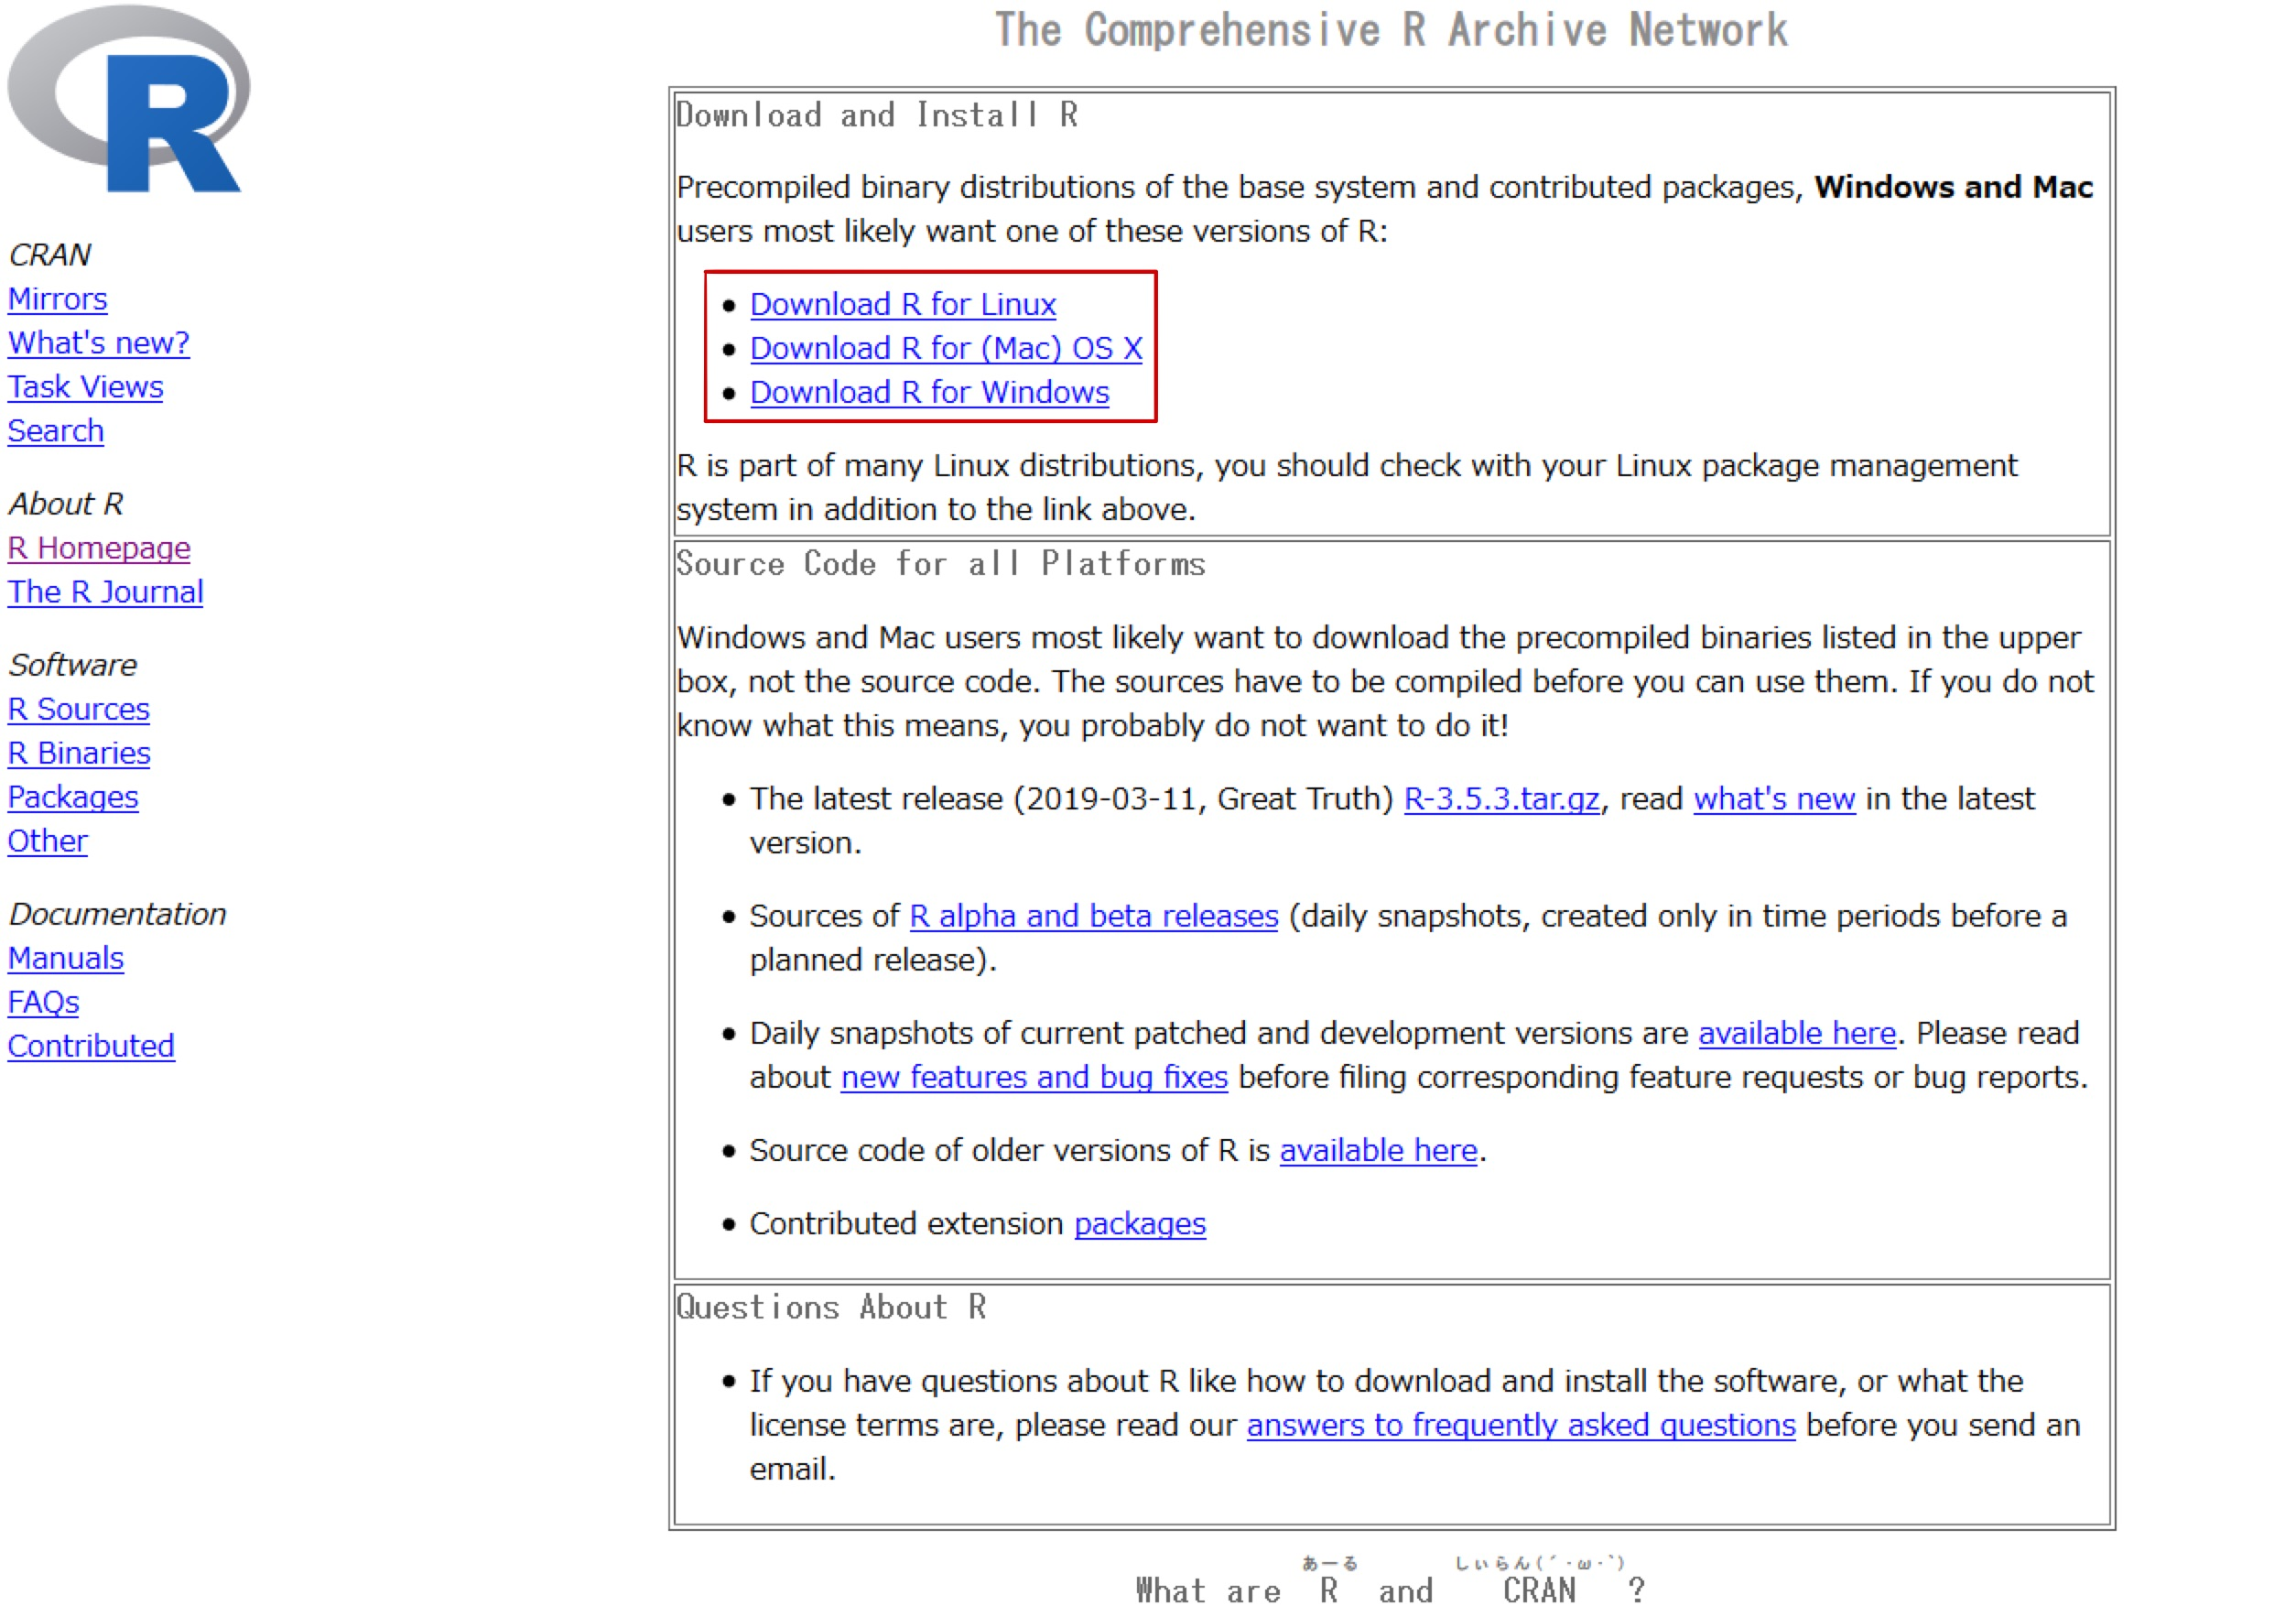
\includegraphics{figures/R3.jpg}

\hypertarget{windowsux306eux5834ux5408}{%
\paragraph{Windowsの場合}\label{windowsux306eux5834ux5408}}

\texttt{install\ R\ for\ the\ first\ time}を選択します。

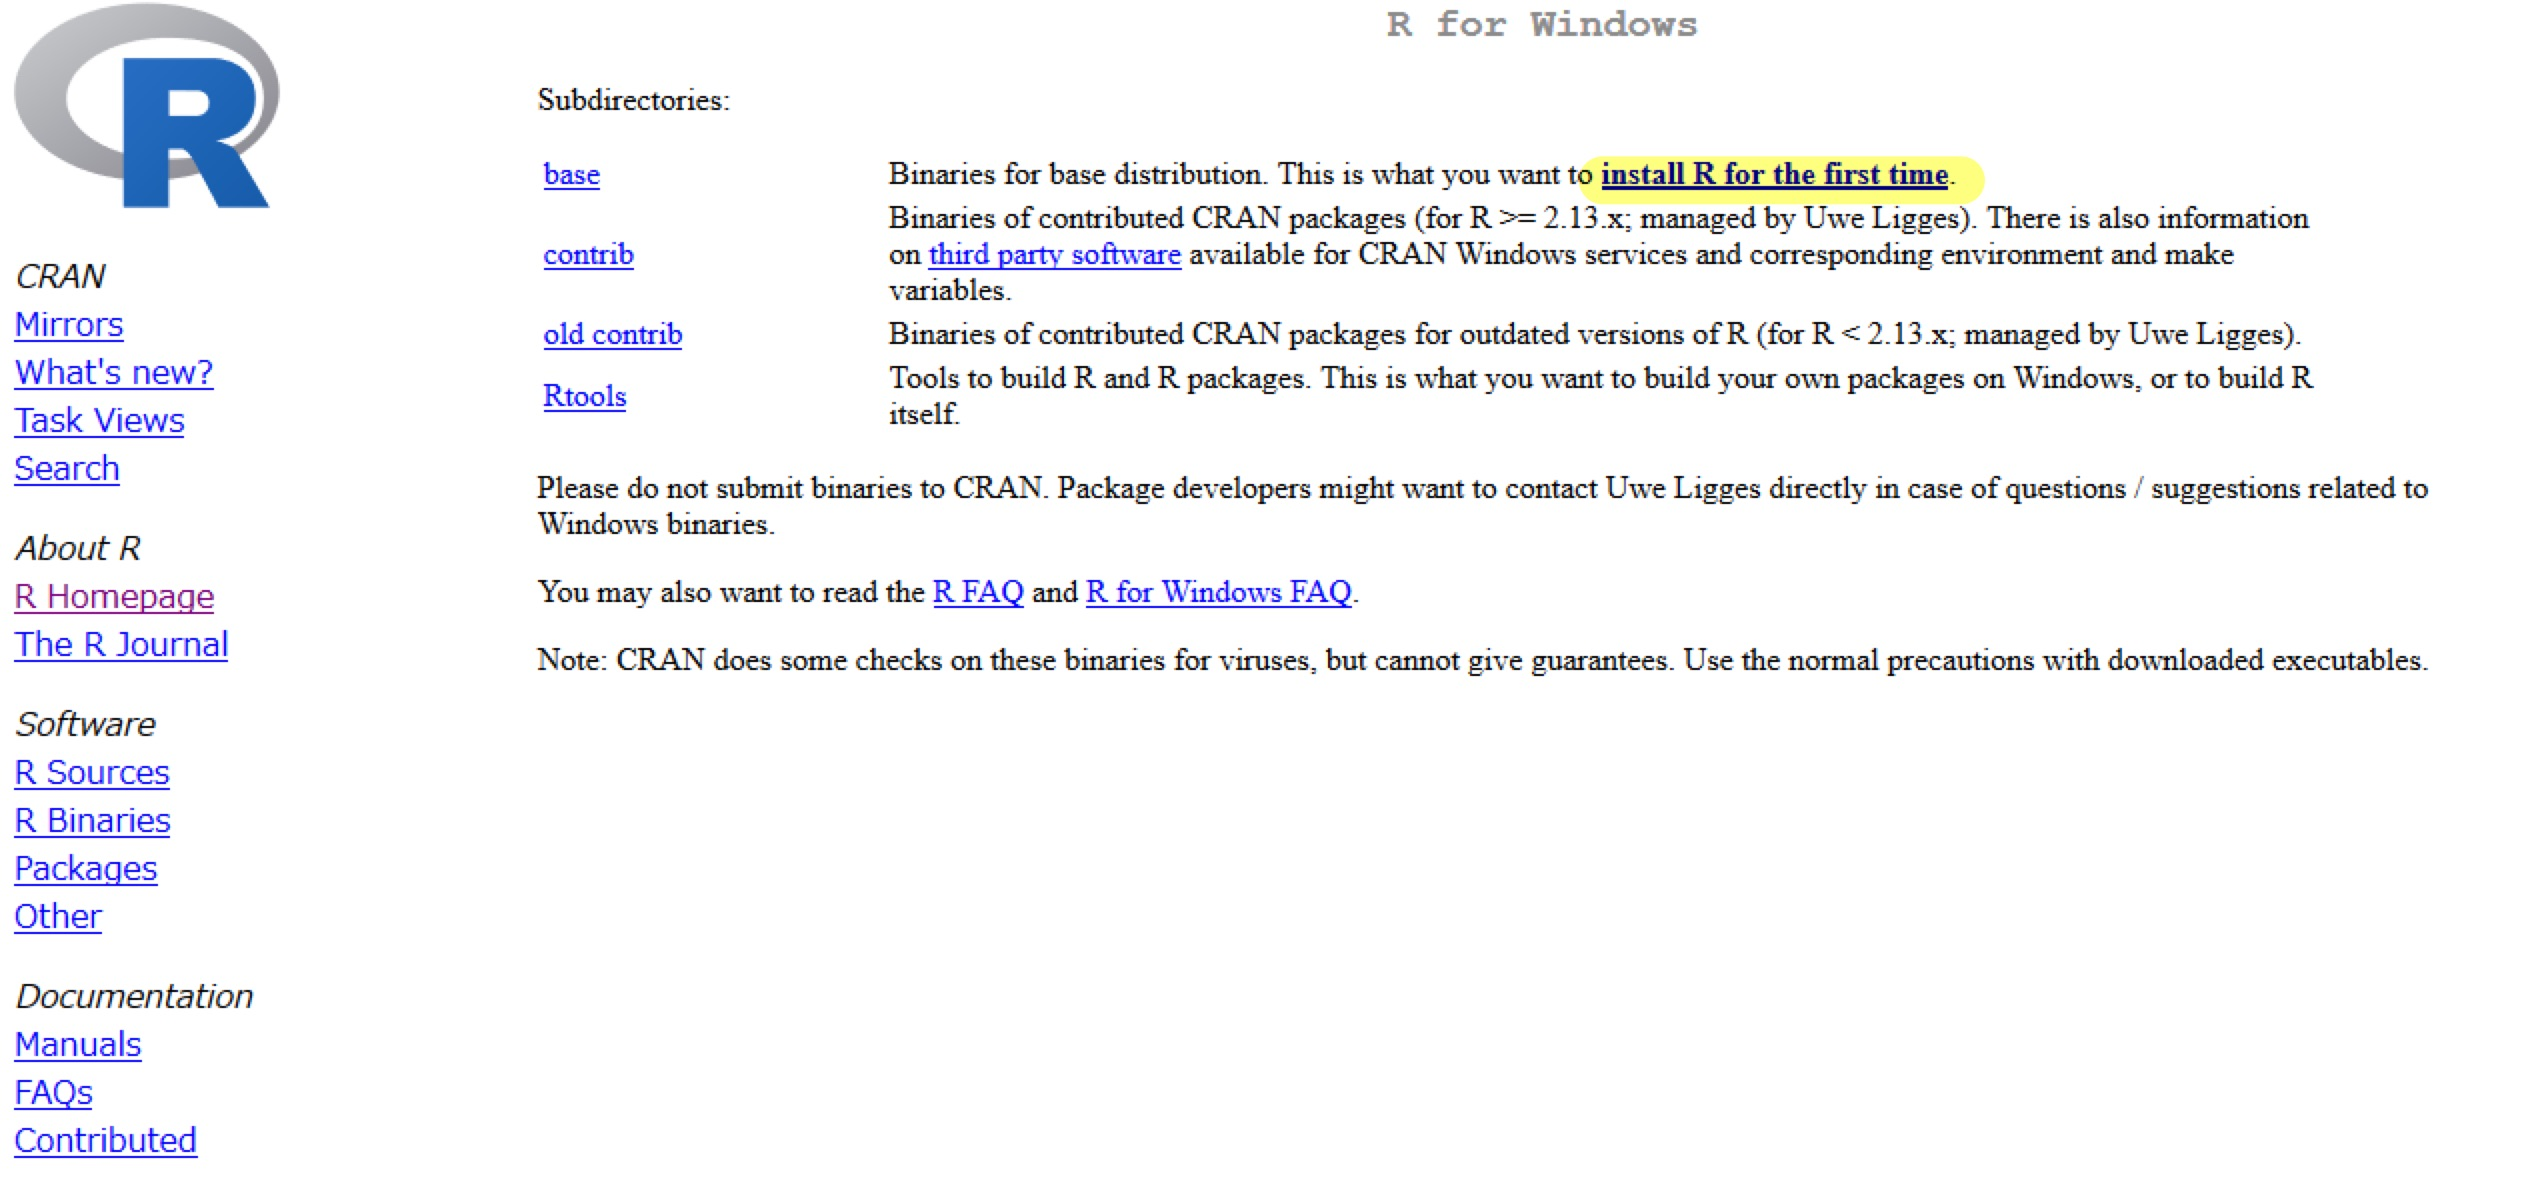
\includegraphics{figures/R4.jpg}

\texttt{Downlosd\ R\ X.X.X\ for\ YYY}を選択してダウンロードします。

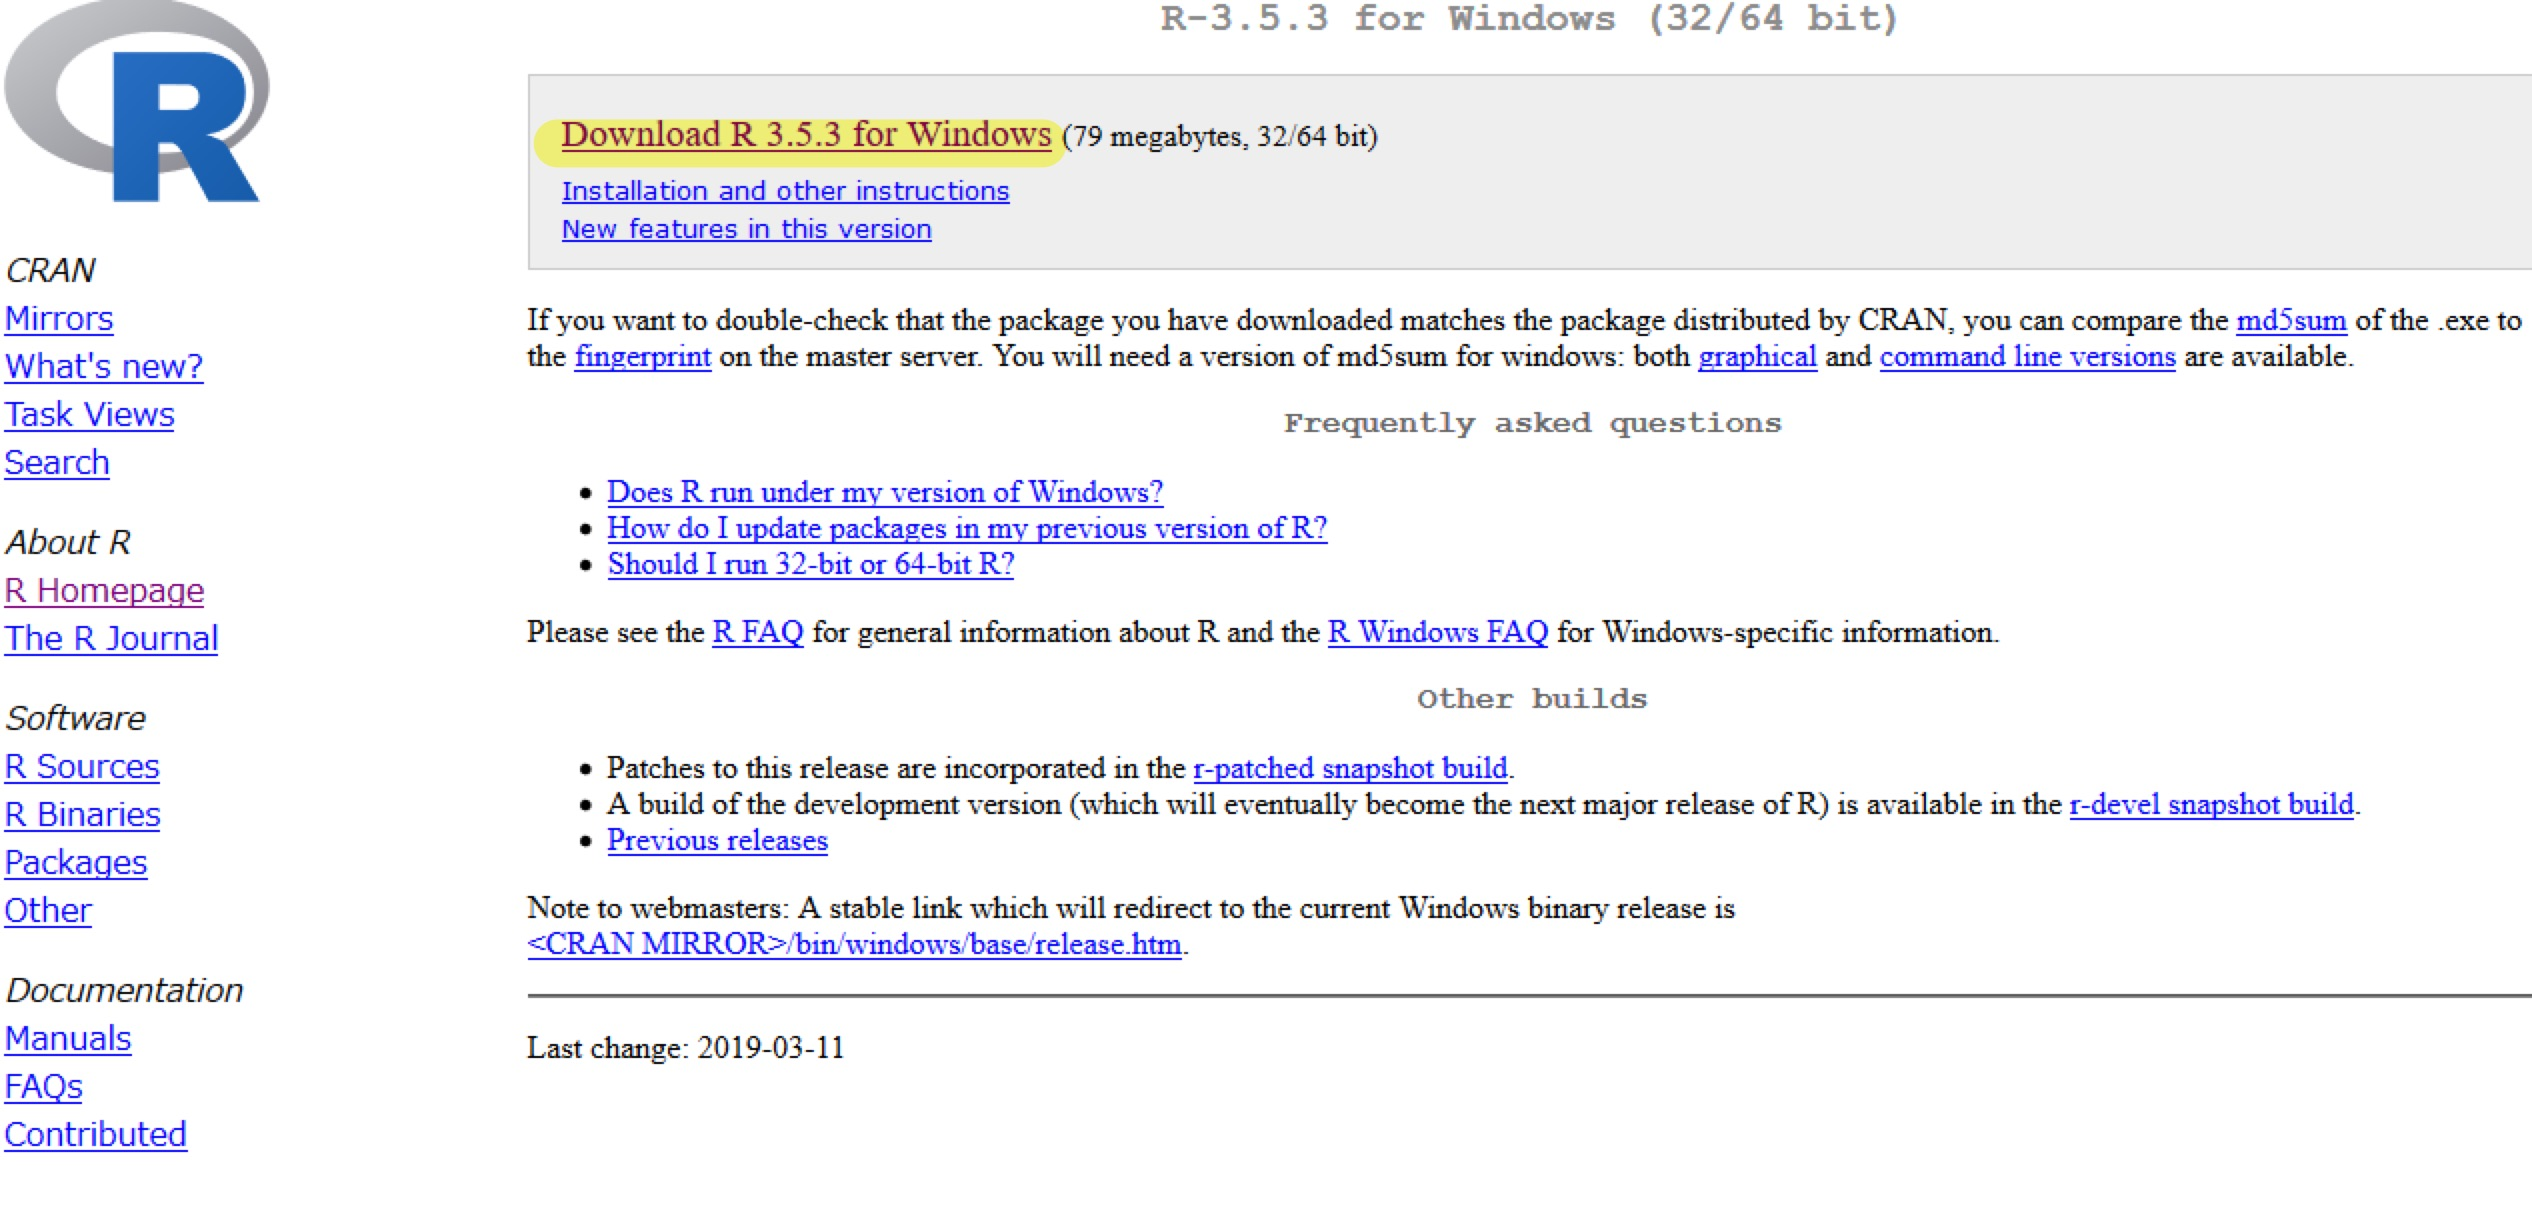
\includegraphics{figures/R5.jpg}

分かりやすいようにダウンロードフォルダにダウンロードしておきます。

Windowsの場合、Rtoolsをインストールもインストールしておきましょう。

\hypertarget{macintoshux306eux5834ux5408}{%
\paragraph{Macintoshの場合}\label{macintoshux306eux5834ux5408}}

\hypertarget{ux30a4ux30f3ux30b9ux30c8ux30fcux30eb}{%
\subsubsection{インストール}\label{ux30a4ux30f3ux30b9ux30c8ux30fcux30eb}}

Rをダウンロードしたフォルダを開き、ファイルをクリックします。

\begin{itemize}
\tightlist
\item
  ファイル名はOSによって異なります。
\end{itemize}

その後は表示されるままに進めていけばよいです。

Rは基本的にOSの言語で表示されますが、英語で使いたい場合は\texttt{Message\ Translations}のインストールにチェックが入っている場合は外しておきましょう。

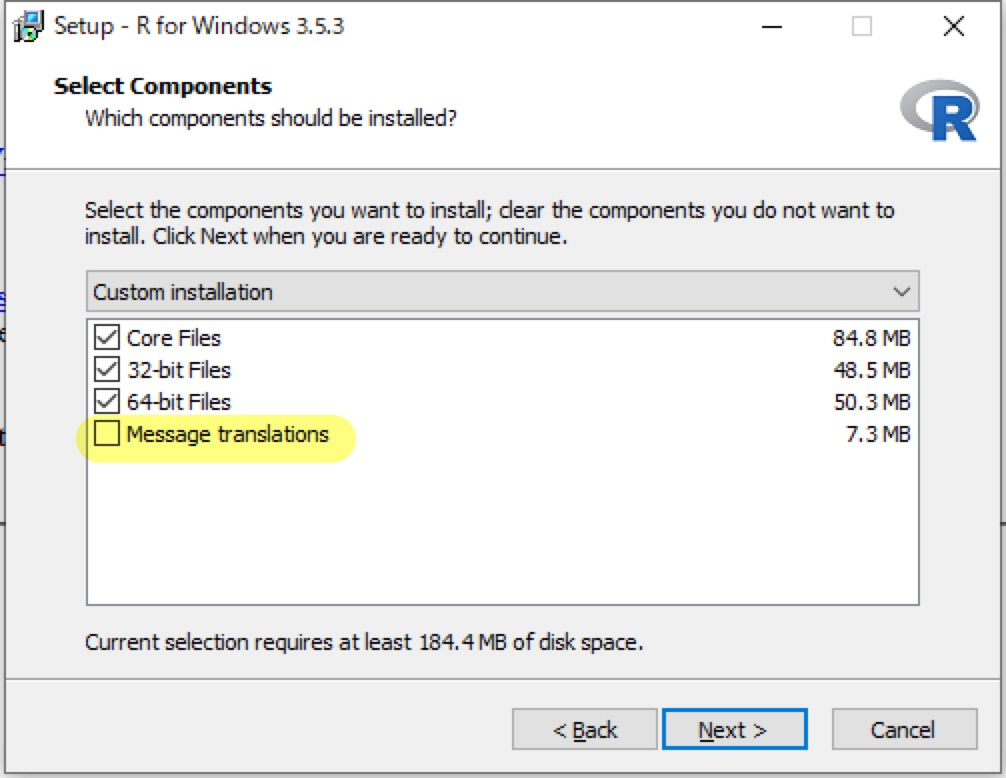
\includegraphics{figures/R6.jpg}

\begin{itemize}
\tightlist
\item
  英語のエラーメッセージで検索したほうが解決策が見つけやすくなります。
\end{itemize}

\hypertarget{rstudioux306eux30a4ux30f3ux30b9ux30c8ux30fcux30eb}{%
\subsection{RStudioのインストール}\label{rstudioux306eux30a4ux30f3ux30b9ux30c8ux30fcux30eb}}

\hypertarget{ux30c0ux30a6ux30f3ux30edux30fcux30c9-1}{%
\subsubsection{ダウンロード}\label{ux30c0ux30a6ux30f3ux30edux30fcux30c9-1}}

RStudioの\href{https://www.rstudio.com/}{公式サイト}からRStudioのダウンロードサイトへ行きます。

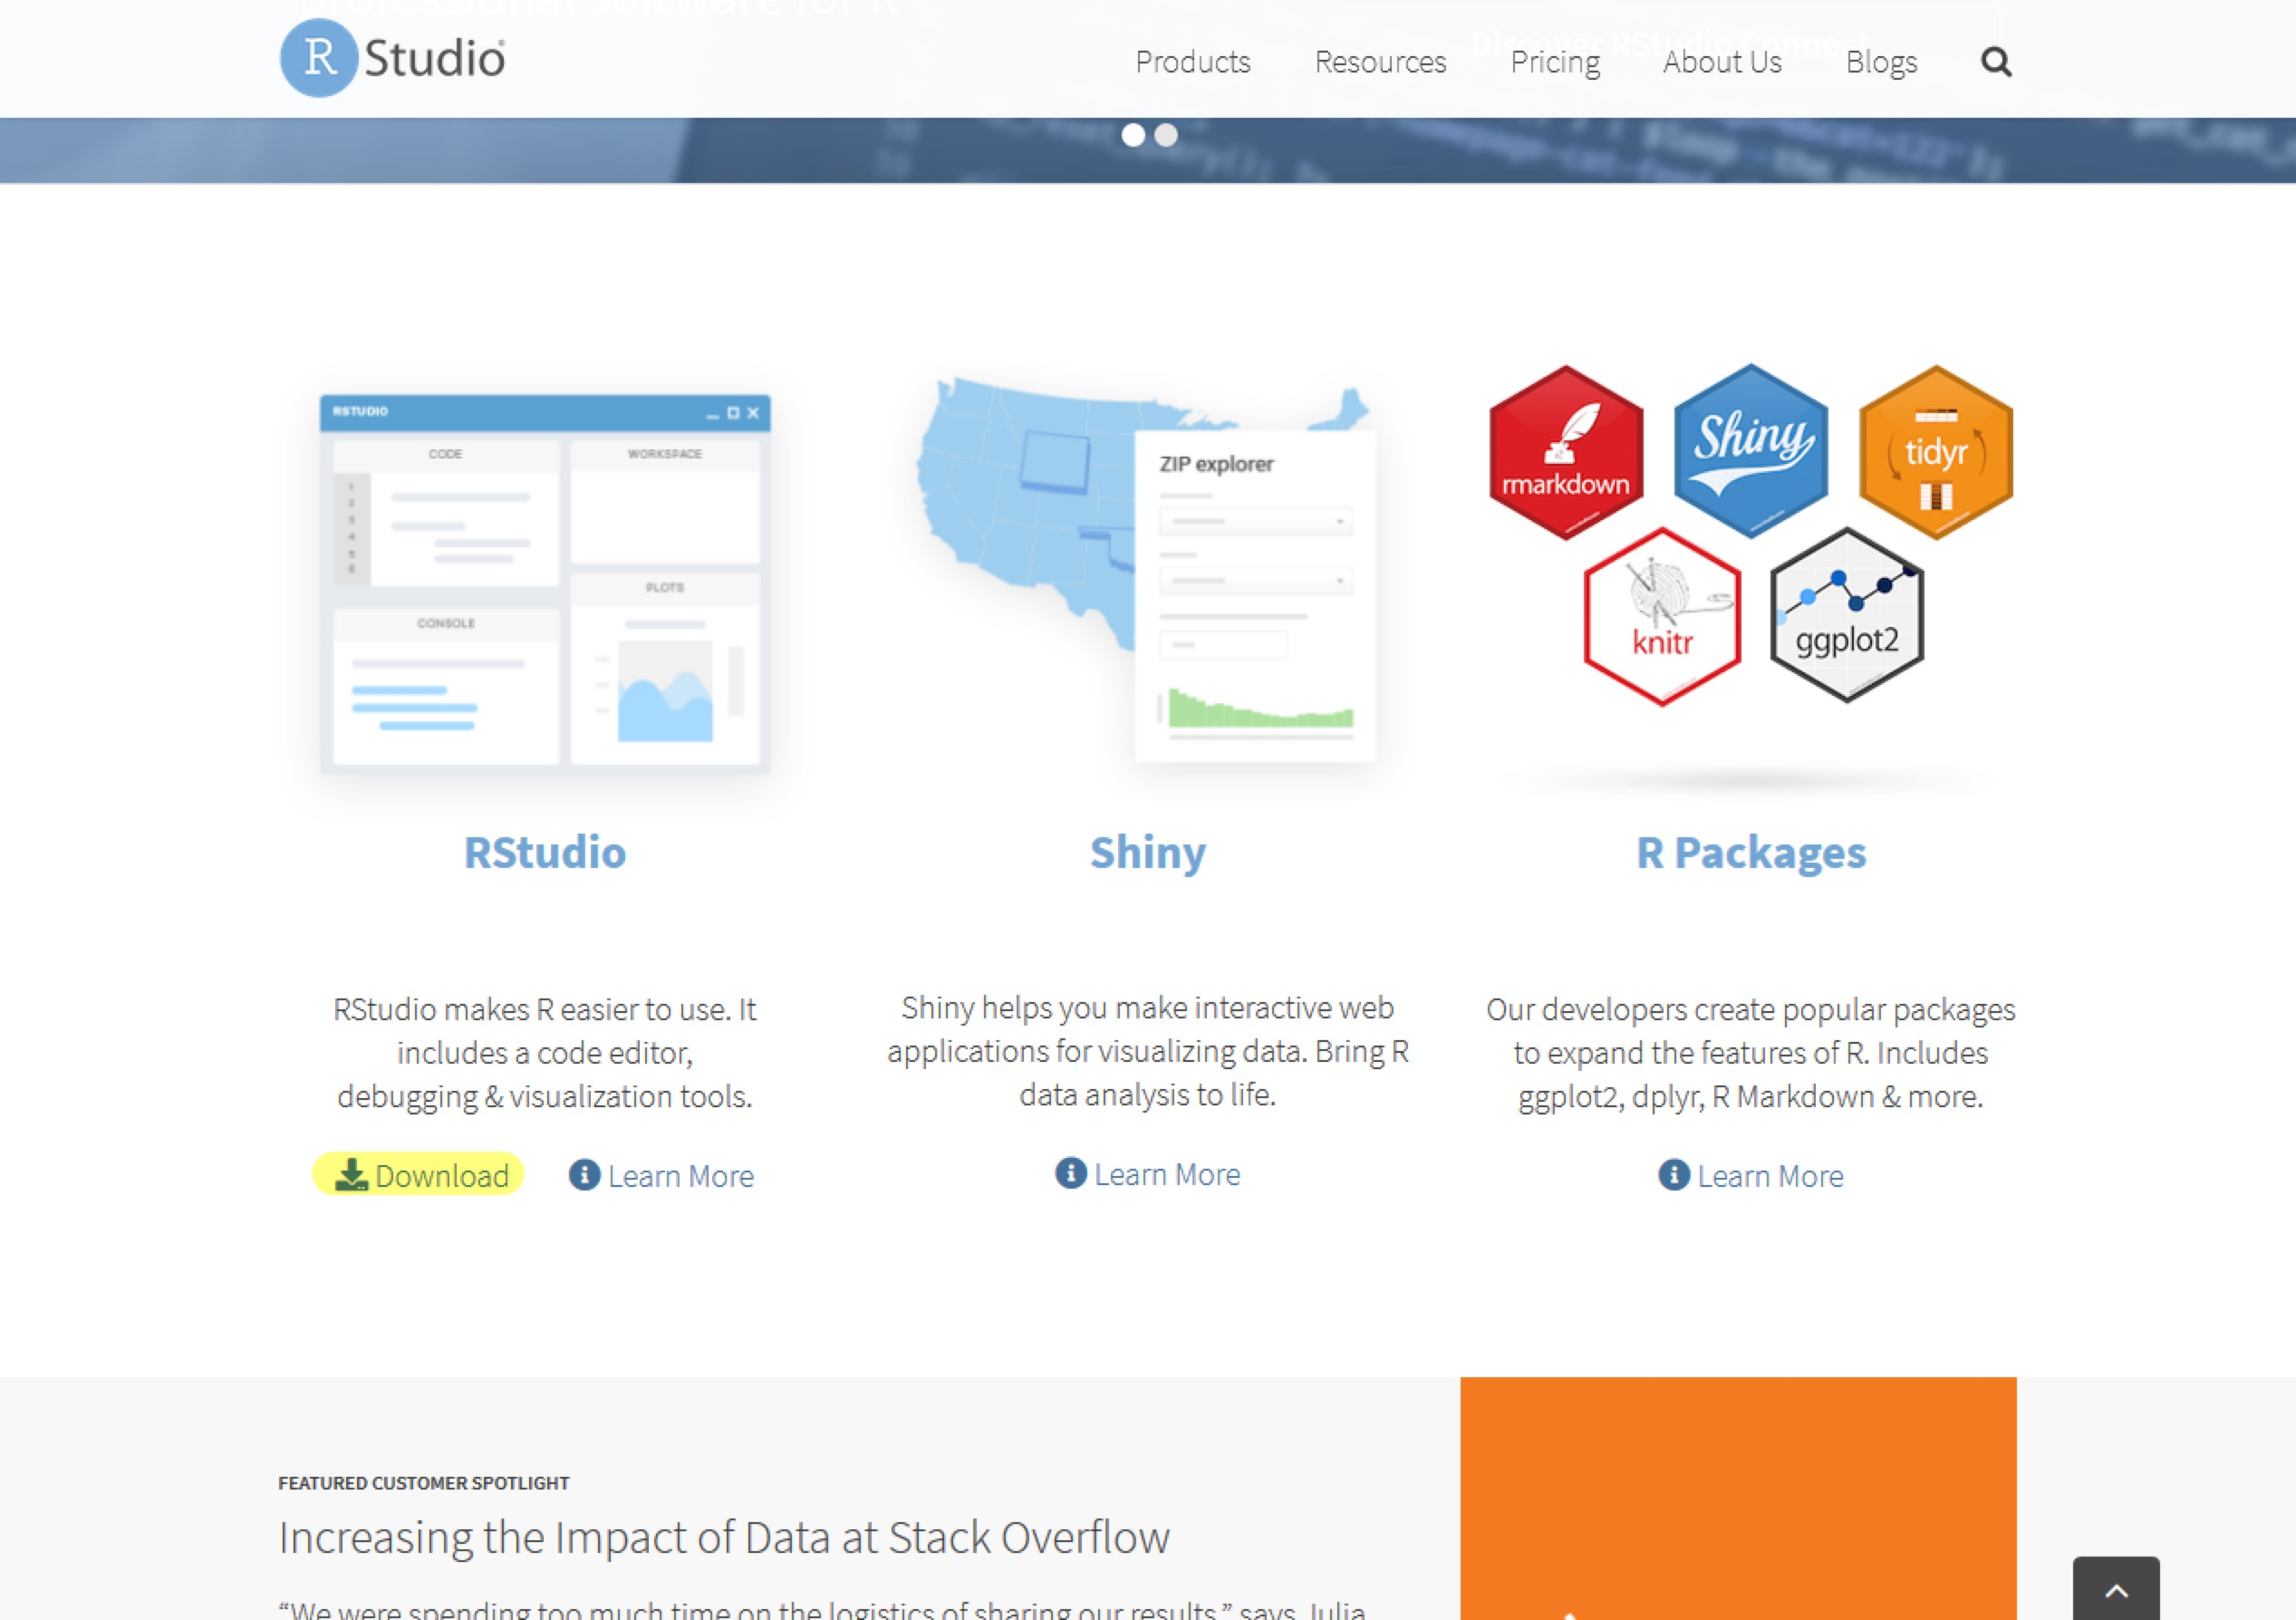
\includegraphics{figures/Rstudio1.jpg}

下の方にインストーラーをダウンロードするリンクがあるのでOSに応じたものを選択します。

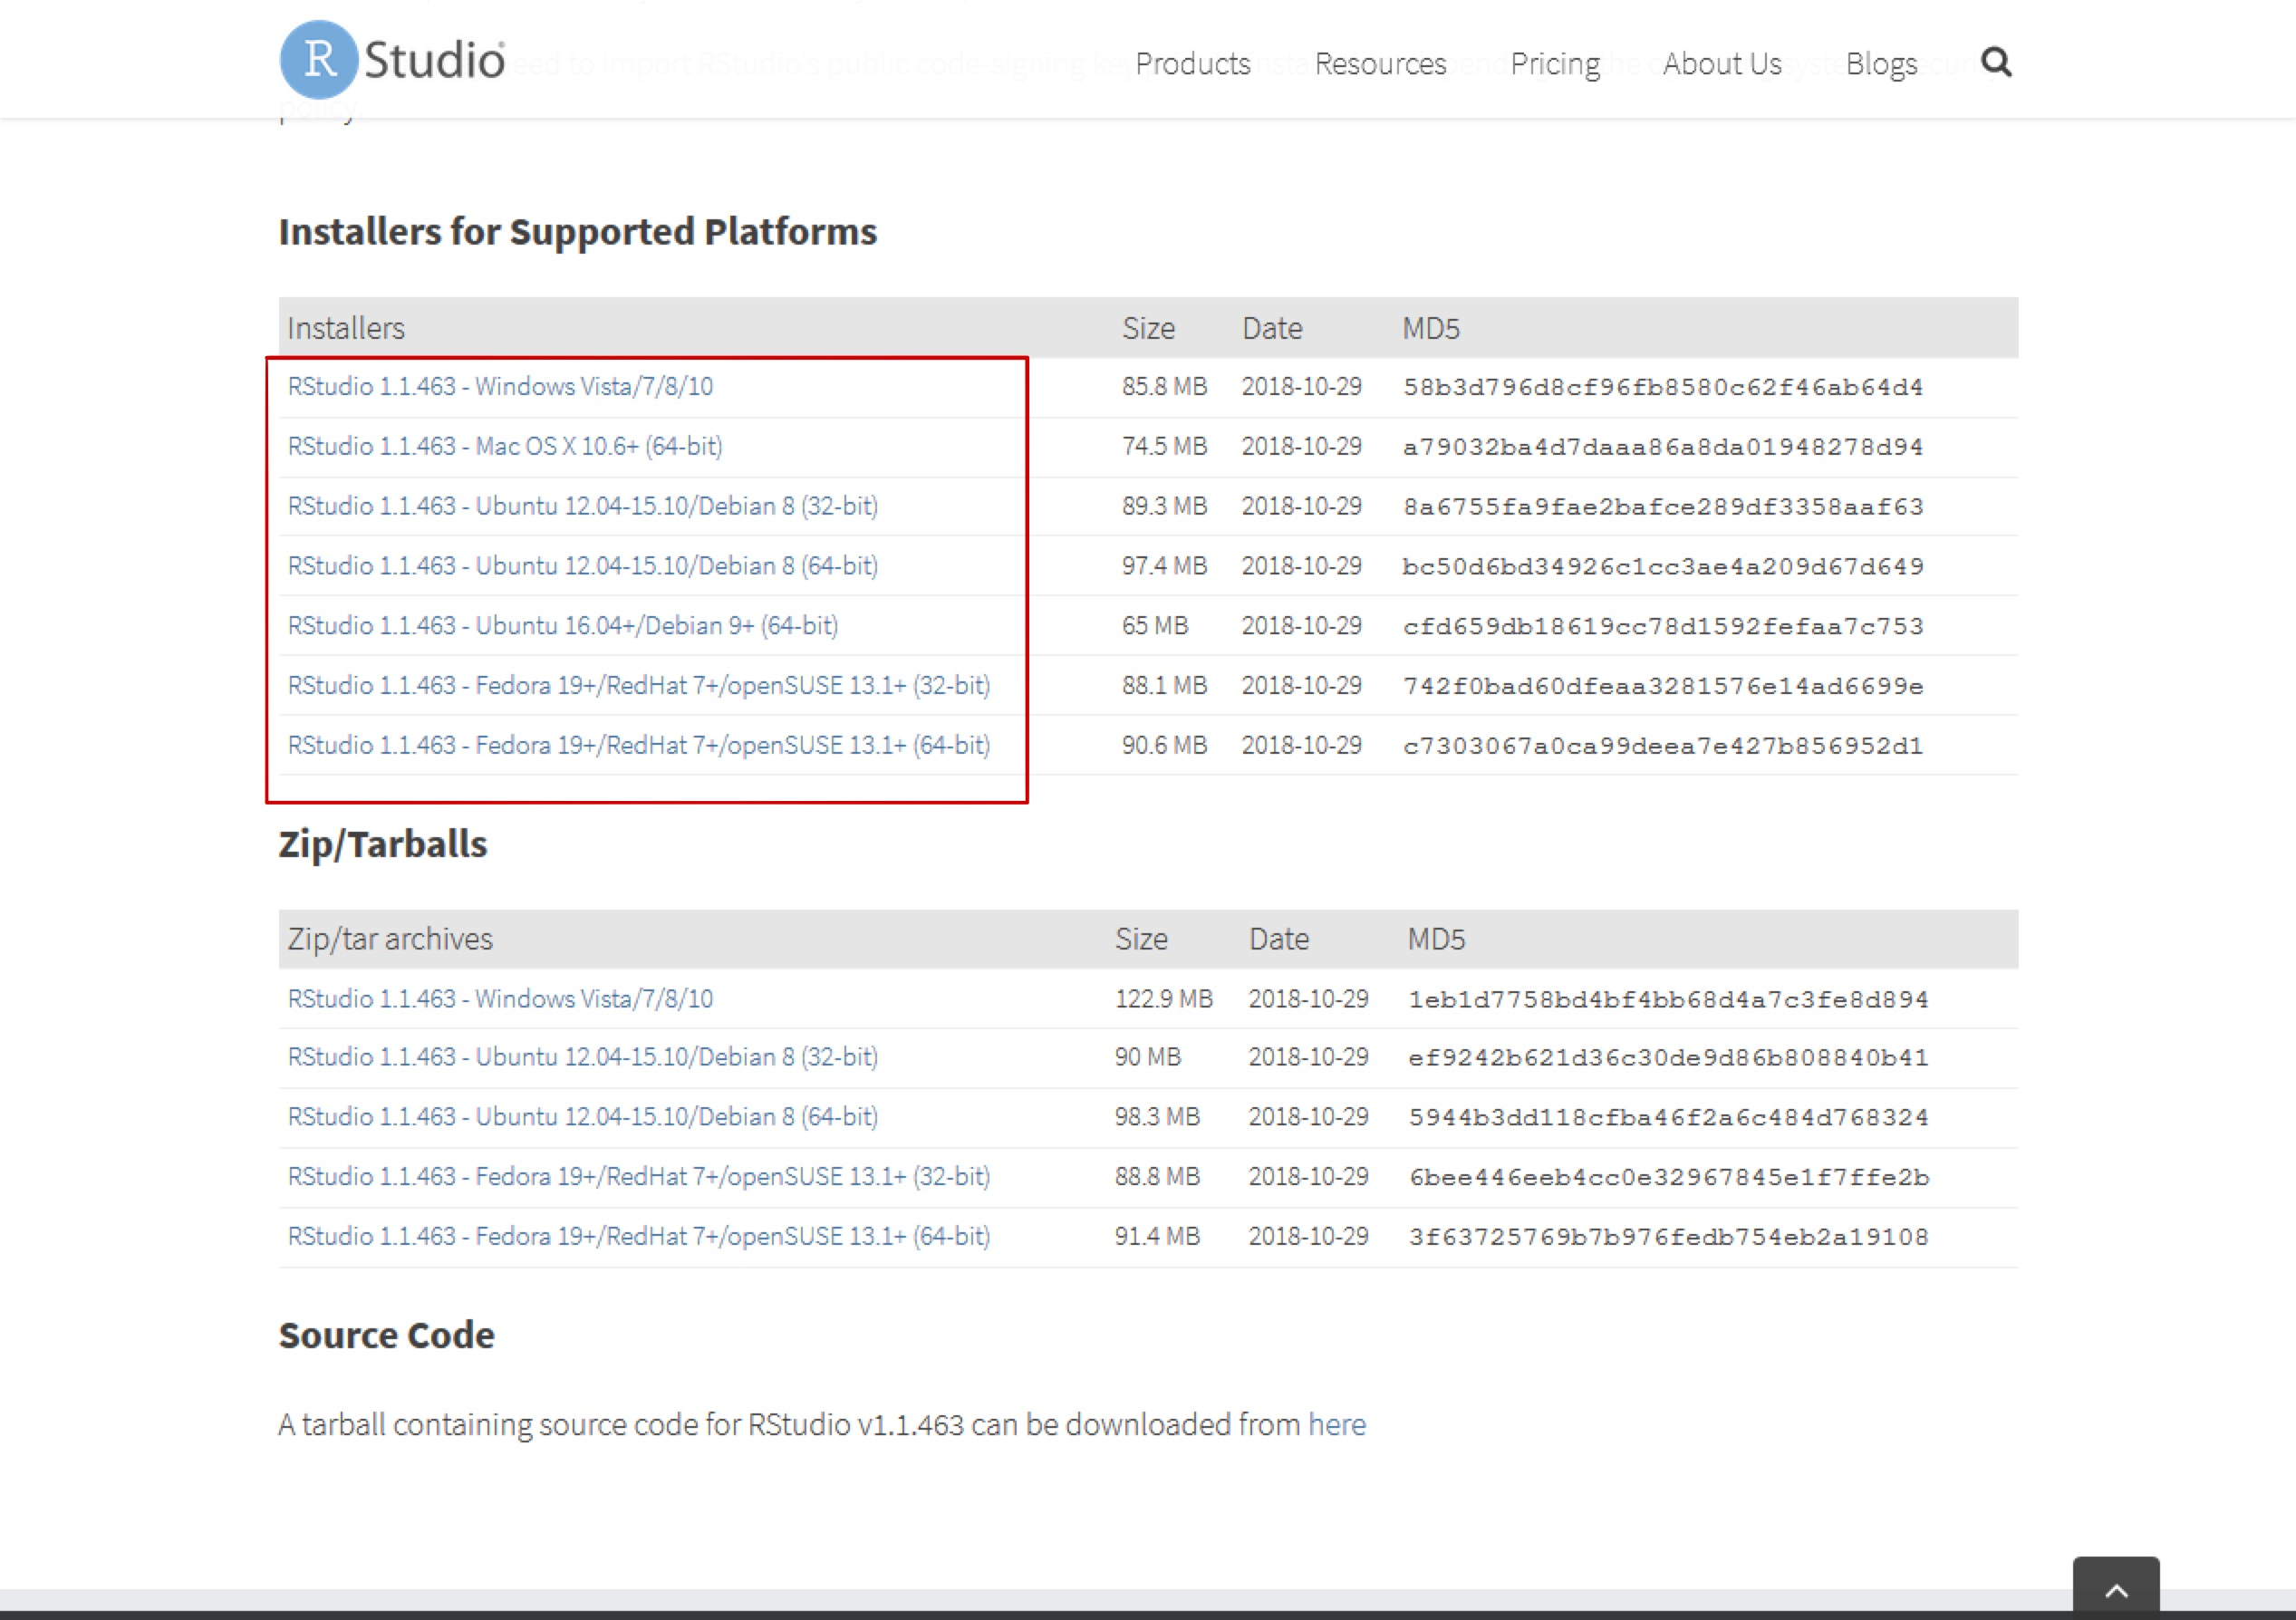
\includegraphics{figures/Rstudio2.jpg}

\begin{itemize}
\tightlist
\item
  安定版ではないけれど最新のRStudioを使いたい人は\href{https://www.rstudio.com/products/rstudio/download/preview/}{RStudio Preview}をインストールしてください。
\item
  また、RやRStudioをインストールせずにオンラインで使用できる\href{https://rstudio.cloud/}{RStudio Cloud}というものもあります。
\end{itemize}

\hypertarget{ux30a4ux30f3ux30b9ux30c8ux30fcux30eb-1}{%
\subsubsection{インストール}\label{ux30a4ux30f3ux30b9ux30c8ux30fcux30eb-1}}

あとはダウンロードしたフォルダに移り、インストーラーを起動して表示されるがままに進めていきます。

\hypertarget{rstudioux306eux8d77ux52d5}{%
\subsubsection{RStudioの起動}\label{rstudioux306eux8d77ux52d5}}

RStudioのショートカットをクリックしたり、メニューで\texttt{RStudio}と入力してクリックすると起動するはずです。

RStudioを初めて起動すると次のような表示になるとはずです。
左側の大きなパネルで\texttt{R}が表示されていればインストールの成功です。

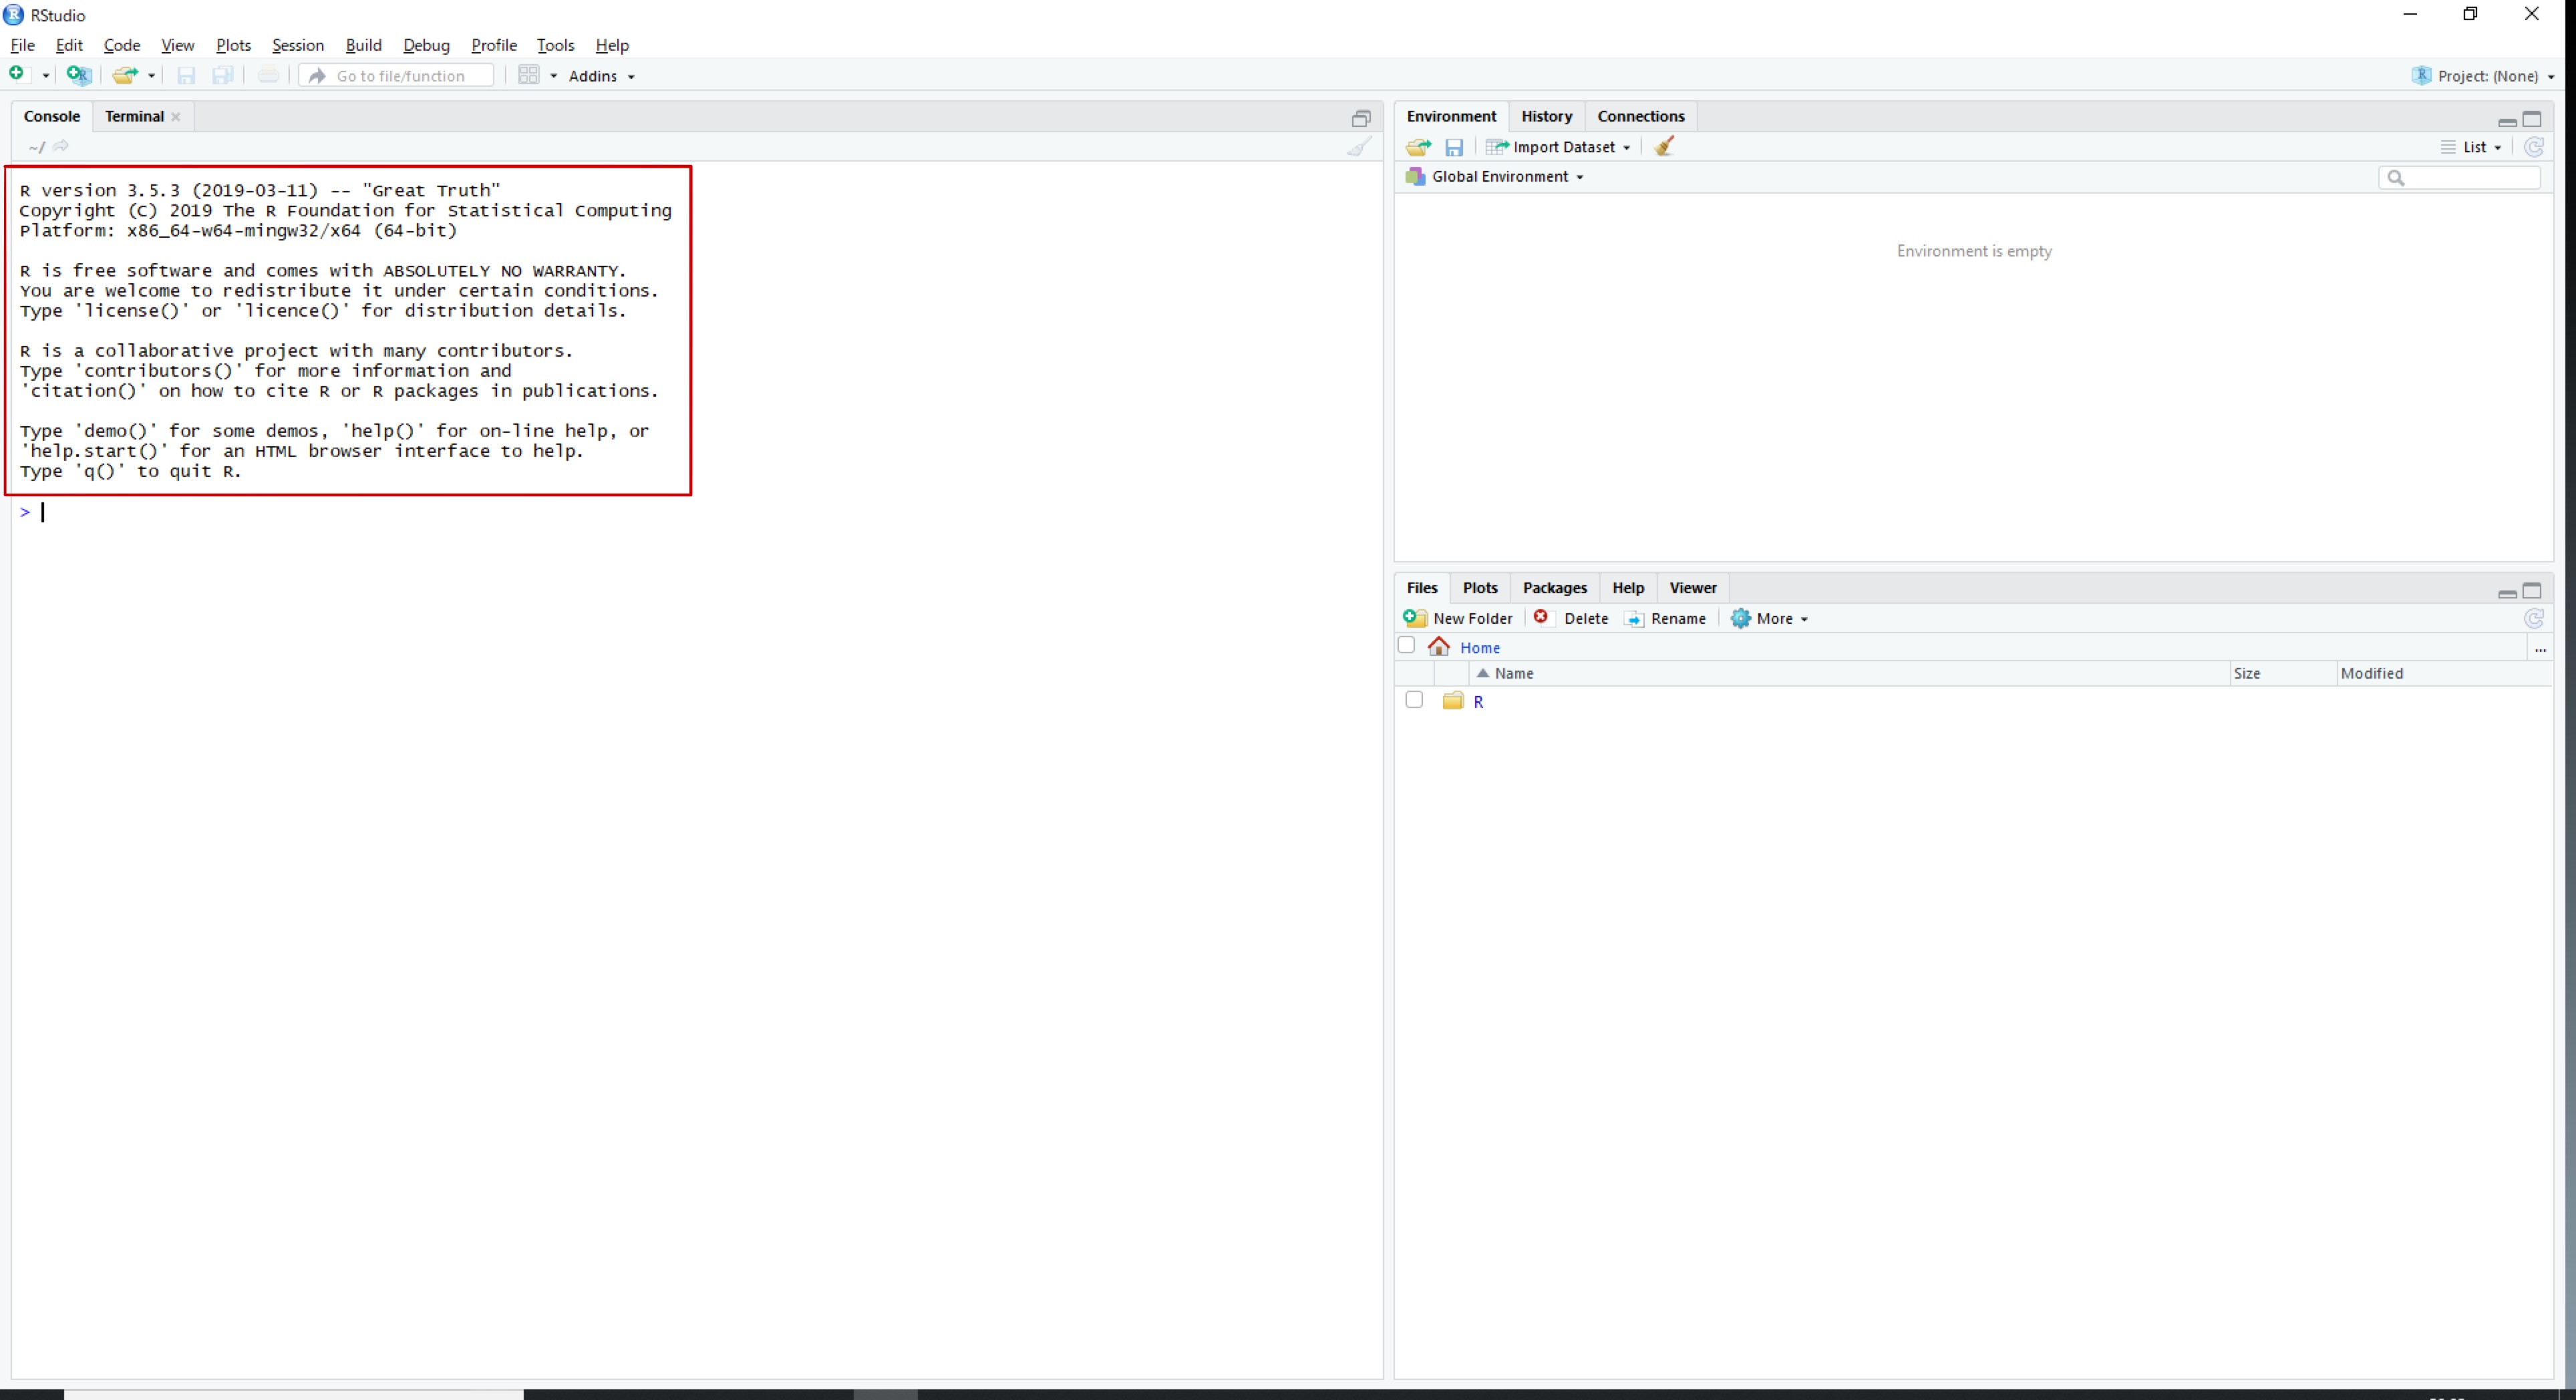
\includegraphics{figures/Rstudio3.jpg}

ちなみに、\texttt{Tools\ \textgreater{}\ Global\ Options\ \textgreater{}\ Appearance}ではフォントや背景・ハイライトの色を変えることができます。

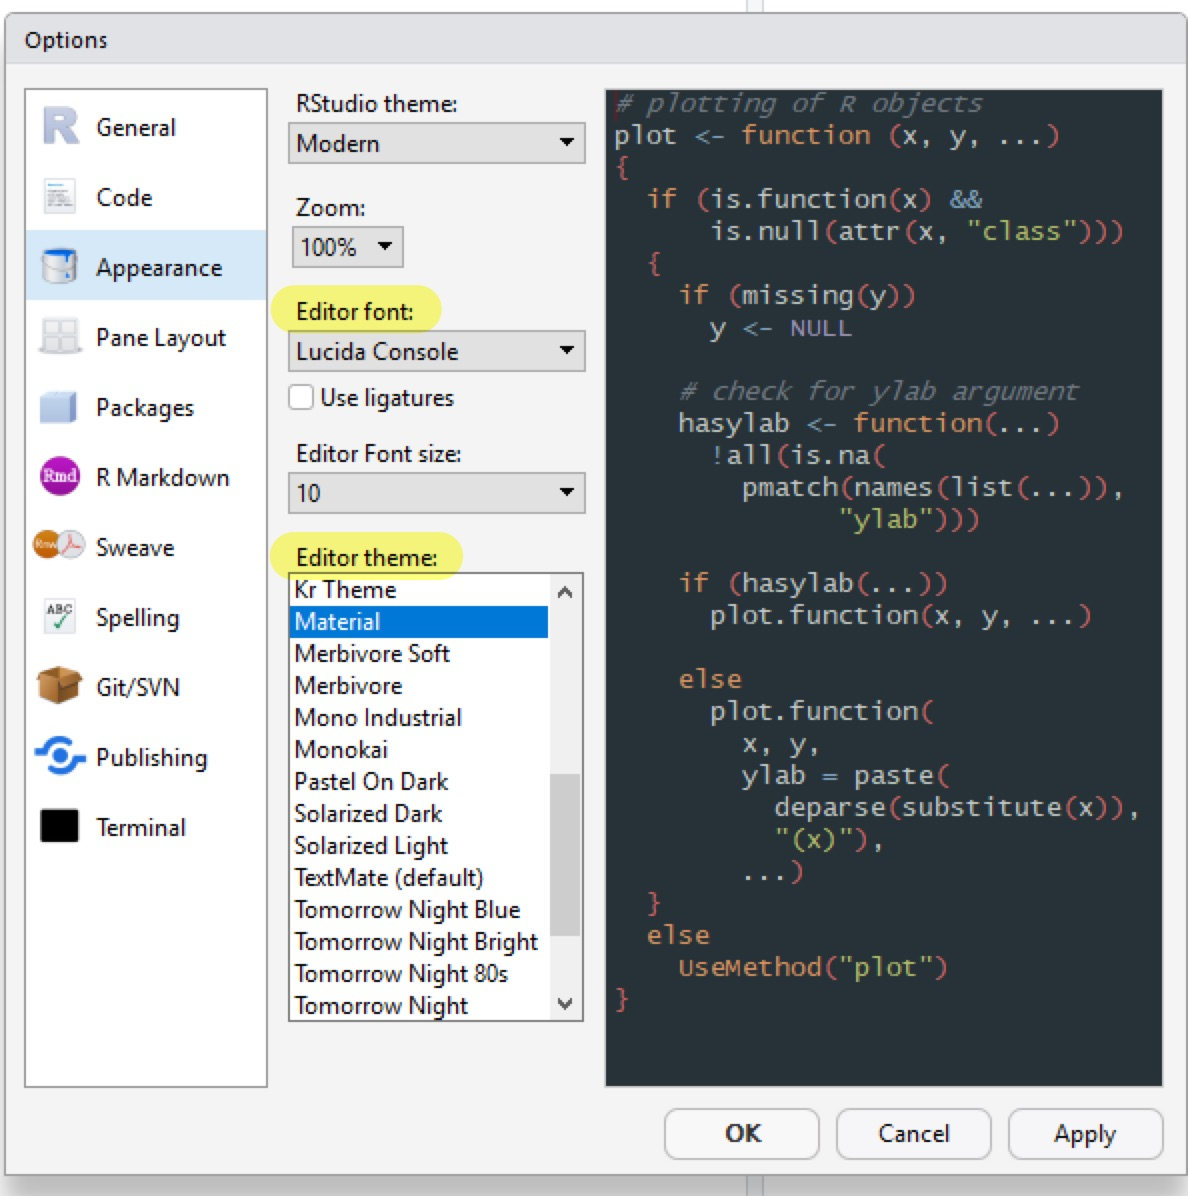
\includegraphics{figures/Rstudio5.jpg}

ダークな背景を選択するとRStudio全体もダークテーマになります。

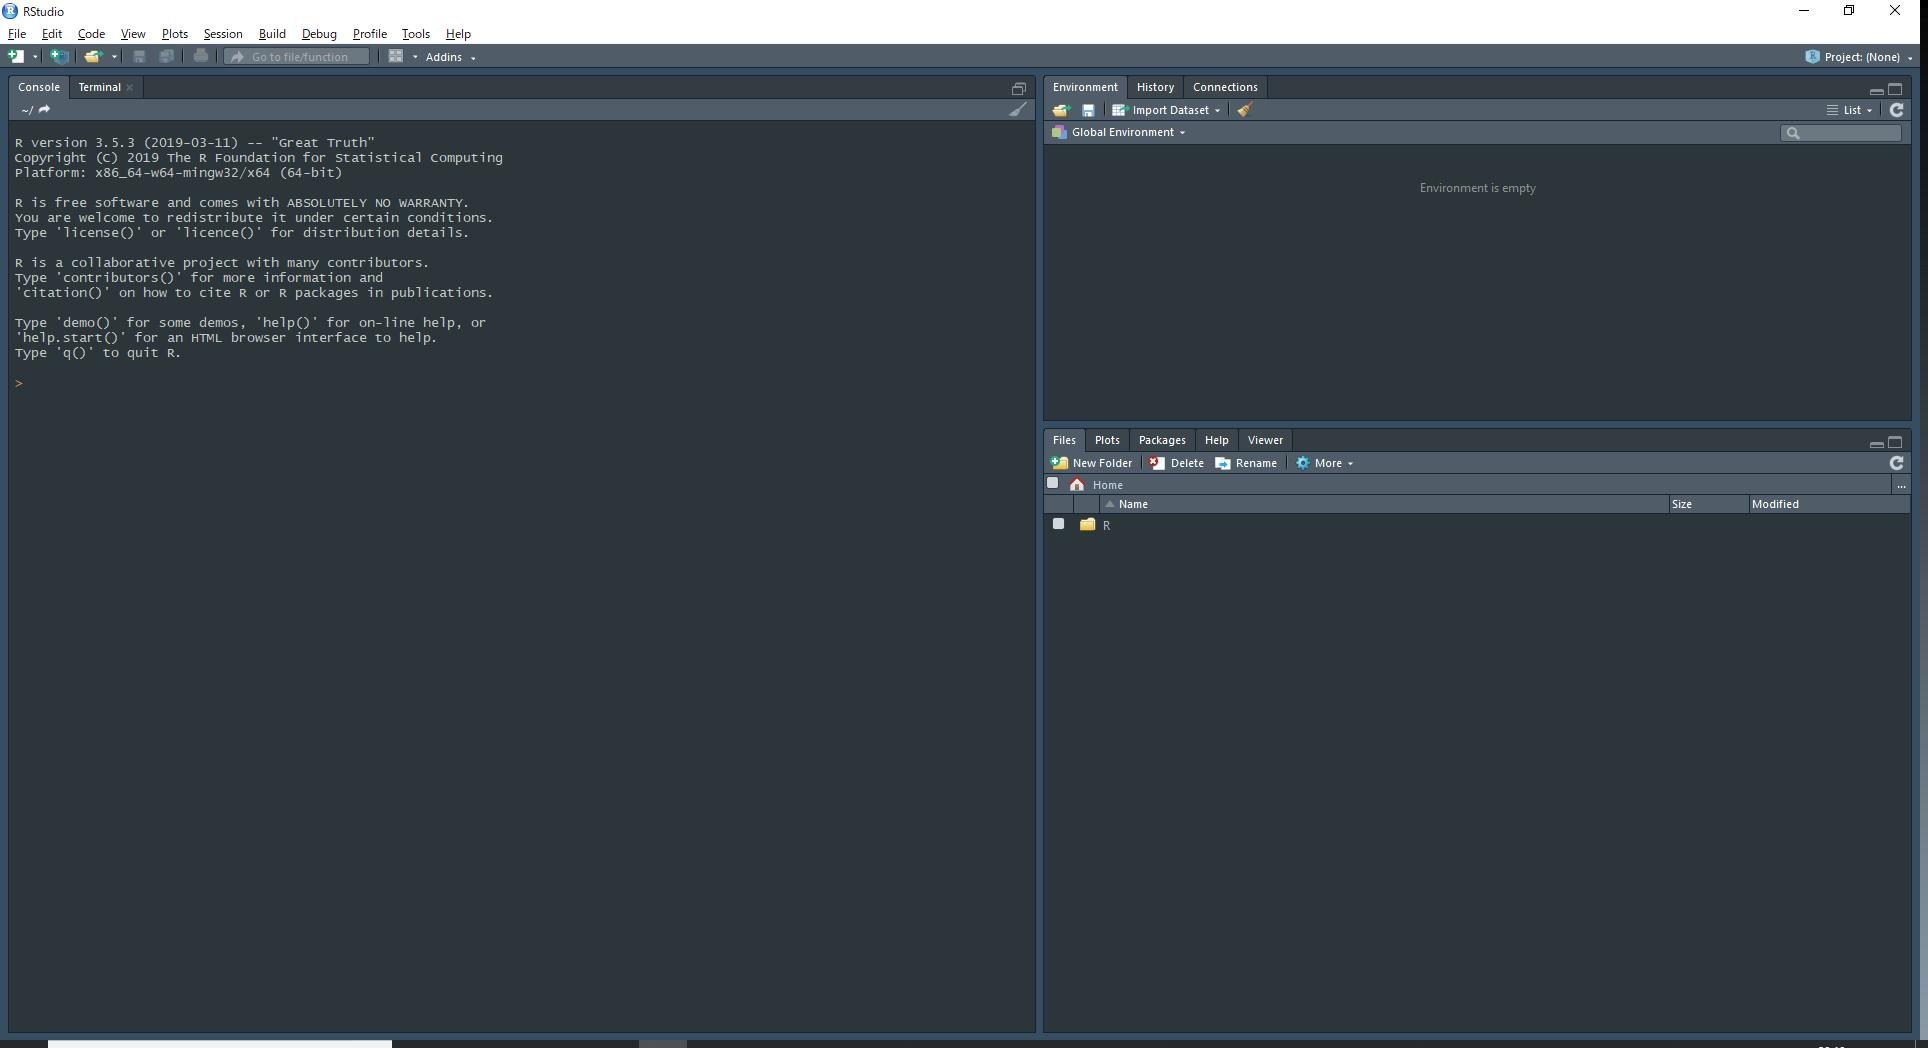
\includegraphics{figures/Rstudio6.jpg}

\hypertarget{rstudio-cloud}{%
\subsubsection{RStudio Cloud*}\label{rstudio-cloud}}

\href{https://rstudio.cloud/}{RStudio CLoud}により、RStudioをブラウザを使ってオンラインで使用することができます。
複数のユーザーで共同作業を行うことも可能です。

\begin{itemize}
\tightlist
\item
  LinuxユーザーはRStudio Serverを使って自らサーバを立てることもできます。
\end{itemize}

\hypertarget{ux518dux73feux53efux80fdux306aux5206ux6790ux306eux305fux3081ux306b}{%
\subsection{再現可能な分析のために}\label{ux518dux73feux53efux80fdux306aux5206ux6790ux306eux305fux3081ux306b}}

再現可能性 (replicability) とは、狭義では、誰がどんな環境で分析しても。オリジナルの分析結果と(ほぼ)同じものを得られることだと思っています。
以下では、再現可能性を担保できるようなR/RStudioの使い方を解説します。

\hypertarget{rux30b9ux30afux30eaux30d7ux30c8}{%
\subsubsection{Rスクリプト}\label{rux30b9ux30afux30eaux30d7ux30c8}}

まず、分析の手順を記録に残し、公開する必要があります。
RではRスクリプトと呼ばれるファイル(拡張子は\texttt{.R})を作成し、そこにコードを残して起きます。

\begin{itemize}
\tightlist
\item
  もちろん、使用したデータも公開する必要があるのは言うまでもありません。
\end{itemize}

\hypertarget{rux30b9ux30afux30eaux30d7ux30c8ux306eux4f5cux6210}{%
\paragraph{Rスクリプトの作成}\label{rux30b9ux30afux30eaux30d7ux30c8ux306eux4f5cux6210}}

RStudioでは左上の\texttt{File\ \textgreater{}\ New\ File\ \textgreater{}\ RScript}もしくは白い紙に緑色のプラスマークのボタンを押して\texttt{R\ Script}を選択します。

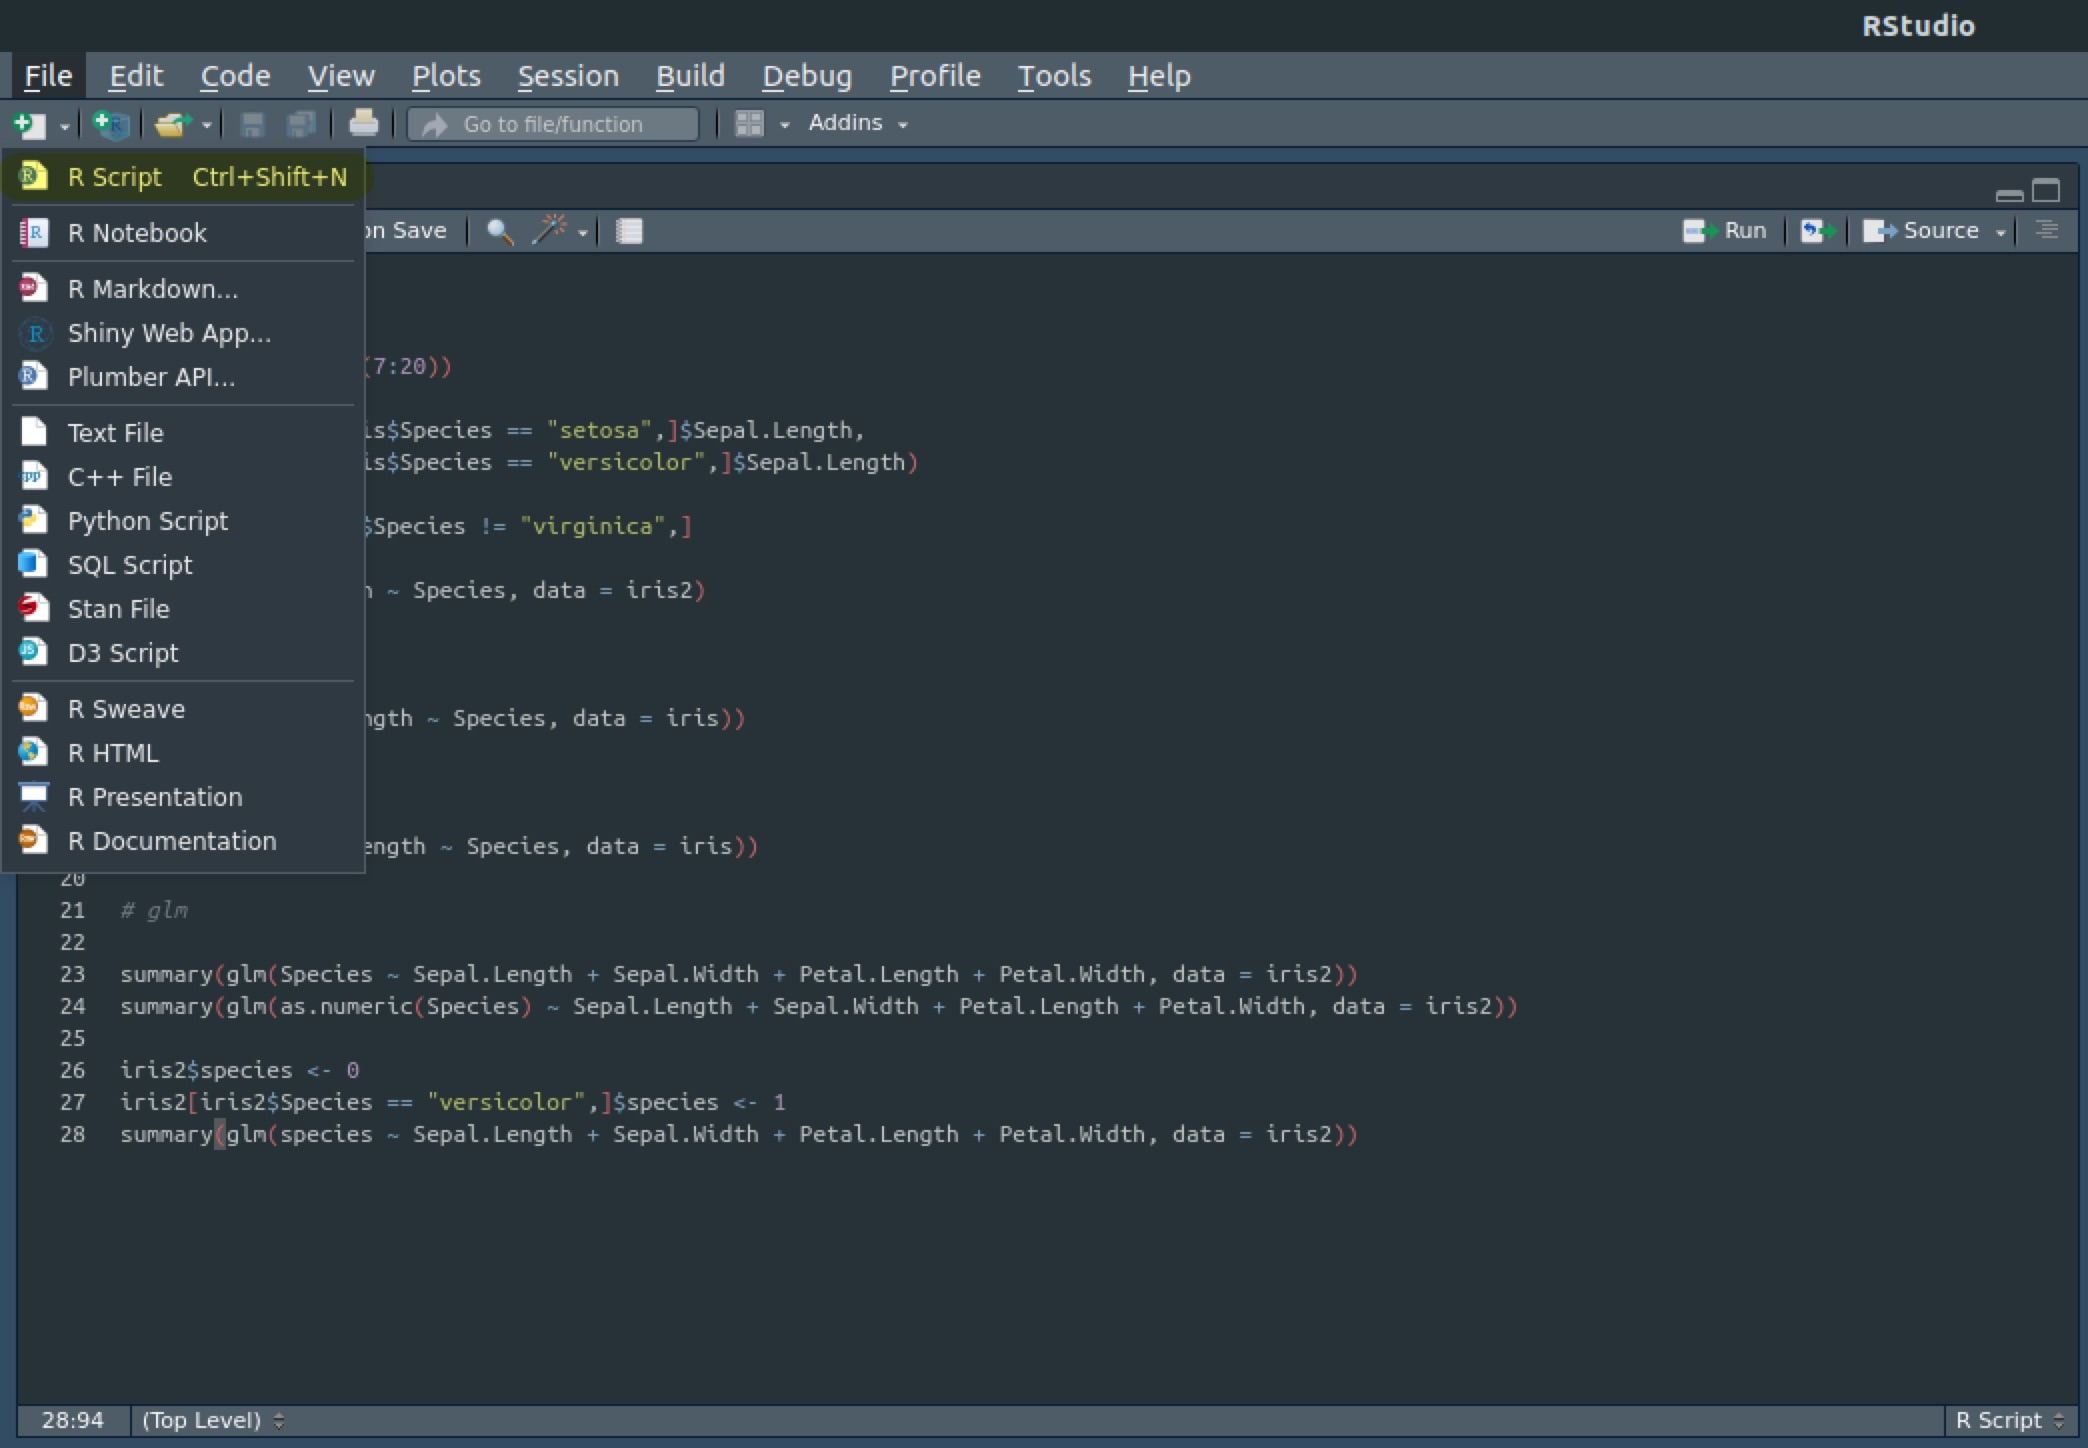
\includegraphics{figures/workflow7.jpg}

すると、デフォルトでは左上のパネルにRスクリプトのエディタが表示されます。

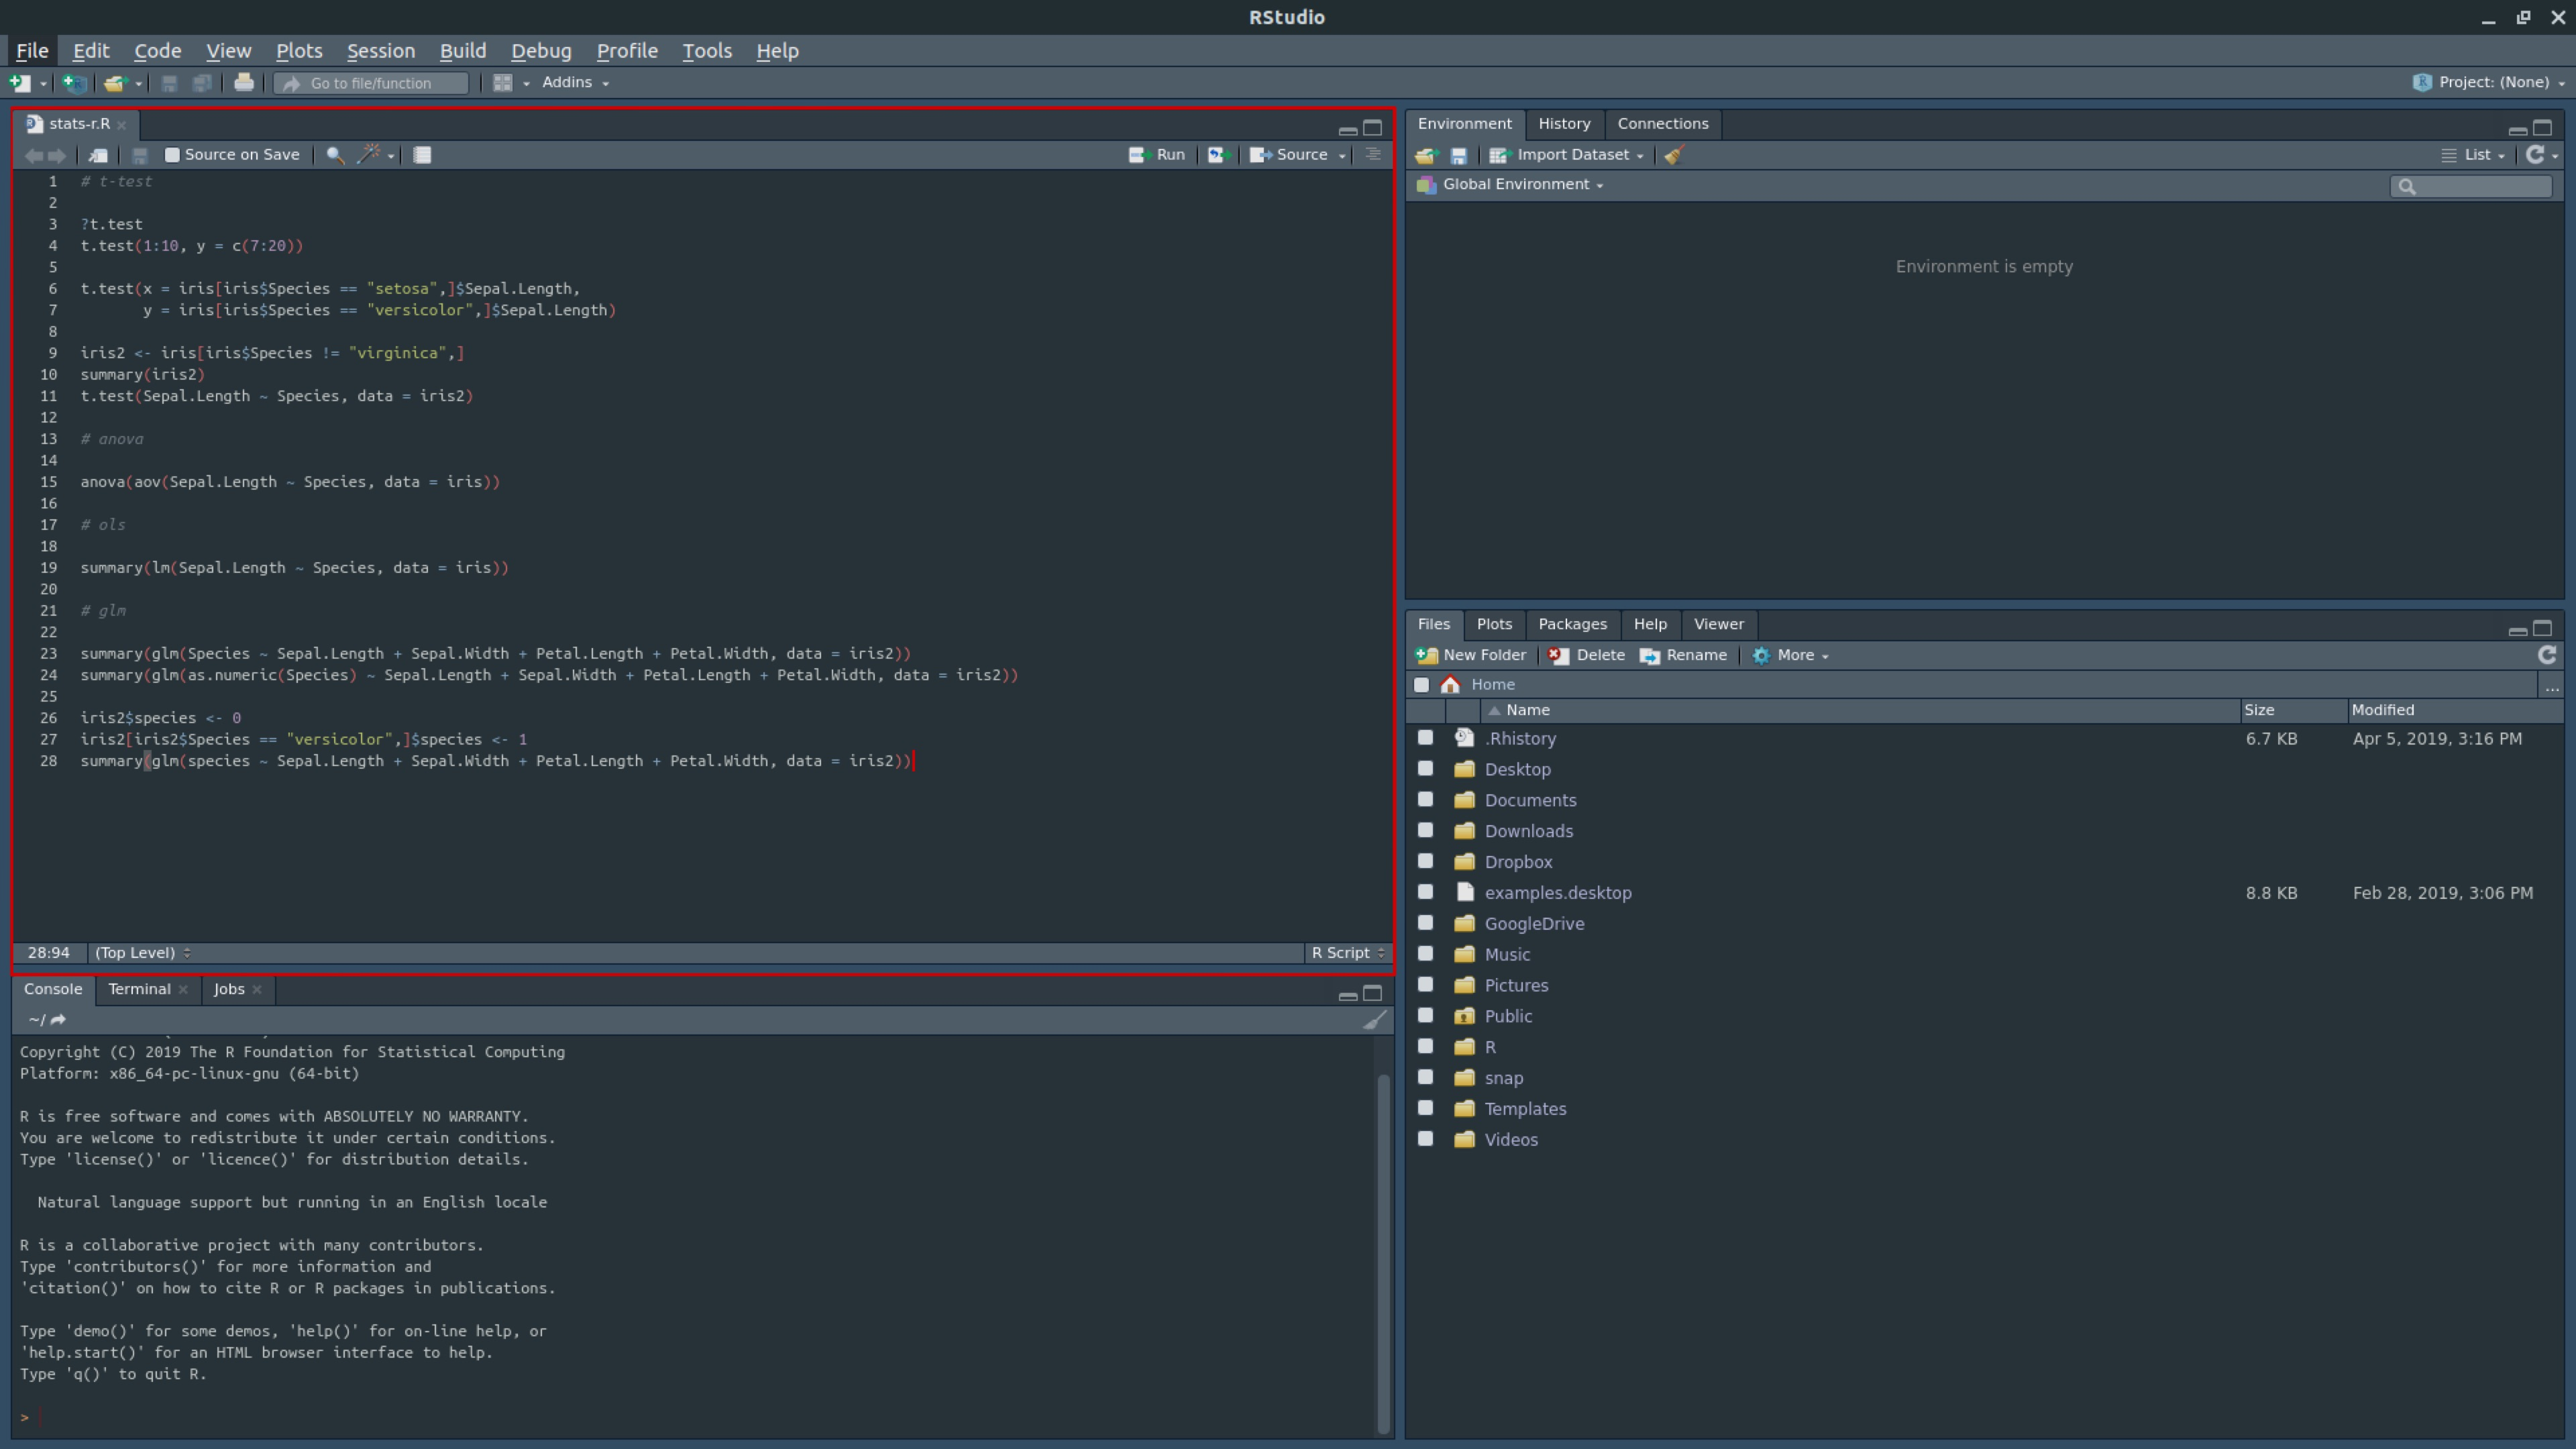
\includegraphics{figures/workflow6.jpg}

\hypertarget{rux30b9ux30afux30eaux30d7ux30c8ux306eux5c55ux958b}{%
\paragraph{Rスクリプトの展開}\label{rux30b9ux30afux30eaux30d7ux30c8ux306eux5c55ux958b}}

RスクリプトをRStudioで開くには左上の\texttt{File\ \textgreater{}\ Open\ File}で選択します。

\hypertarget{rux30b9ux30afux30eaux30d7ux30c8ux306eux5b9fux884c}{%
\paragraph{Rスクリプトの実行}\label{rux30b9ux30afux30eaux30d7ux30c8ux306eux5b9fux884c}}

Rスクリプトに書かれたコードは\texttt{Ctrl\ +\ Enter}を押すと、カーソルのある行がコンソールに流れ、実行されます。

\hypertarget{rux30d7ux30edux30b8ux30a7ux30afux30c8}{%
\subsubsection{Rプロジェクト}\label{rux30d7ux30edux30b8ux30a7ux30afux30c8}}

\protect\hyperlink{data-import}{データの読み込み}で解説したように、データの読み込みや保存の際には起点となる作業ディレクトリ (working directory) を決める必要があります。

一般的に、作業ディレクトリはPCによって変わってしまうので、Rプロジェクトを立てることでその問題を回避します。
簡単に言えば、Rプロジェクトをクリックすることで自動的に作業ディレクトリが設定された状態でRStudioを起動することができます。

また、プロジェクトごとにRStudioを起動できるので、異なるプロジェクト間でデータやRスクリプトが混在することも回避できます。

ひとまず、\textbf{新しい分析を行う際は必ずRプロジェクトを作成する}ようにしましょう。

\hypertarget{rux30d7ux30edux30b8ux30a7ux30afux30c8ux306eux4f5cux6210}{%
\paragraph{Rプロジェクトの作成}\label{rux30d7ux30edux30b8ux30a7ux30afux30c8ux306eux4f5cux6210}}

まずは、プロジェクトの作り方ですが、RStudioの左上の青いボタンをクリックします。

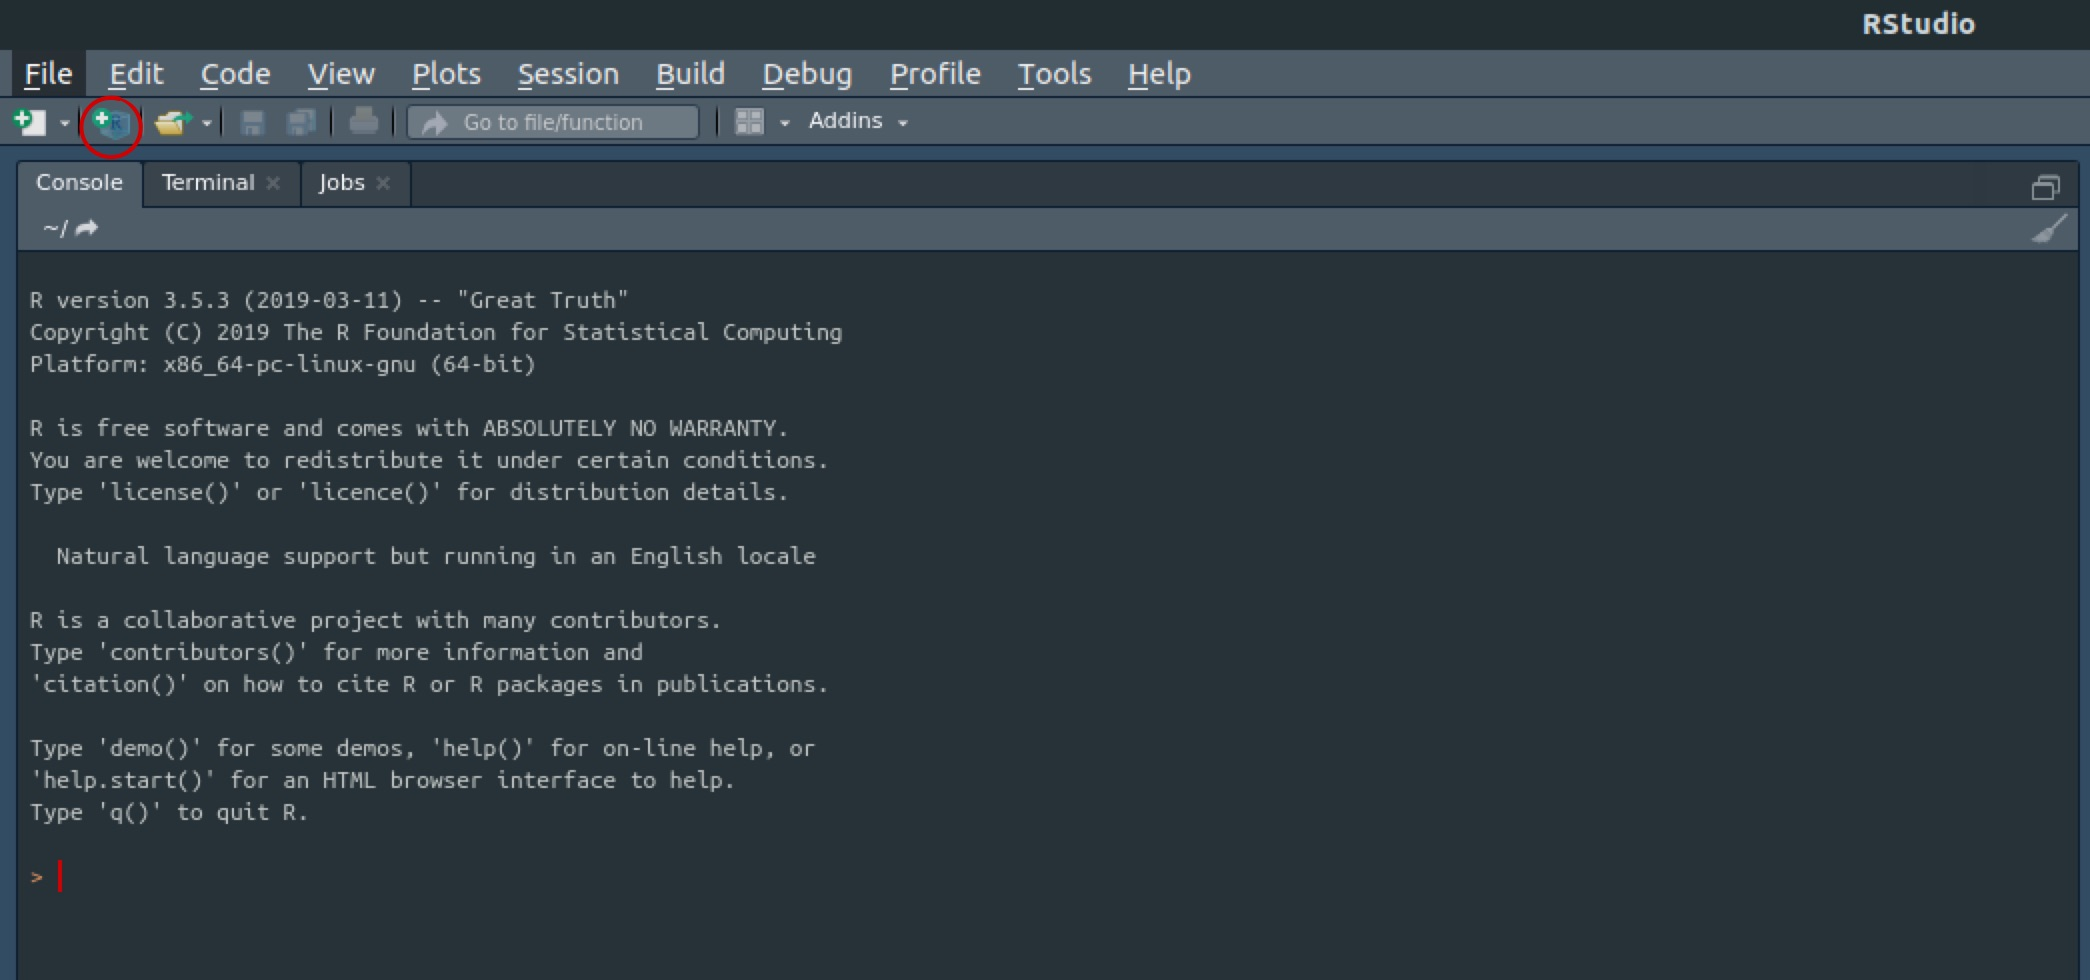
\includegraphics{figures/workflow2.jpg}

続いて、新たにプロジェクト用のフォルダを作るのであれば\texttt{New\ Directory}を、既存のフォルダをプロジェクト用にするのであれば\texttt{Existing\ Directory}を選択します。

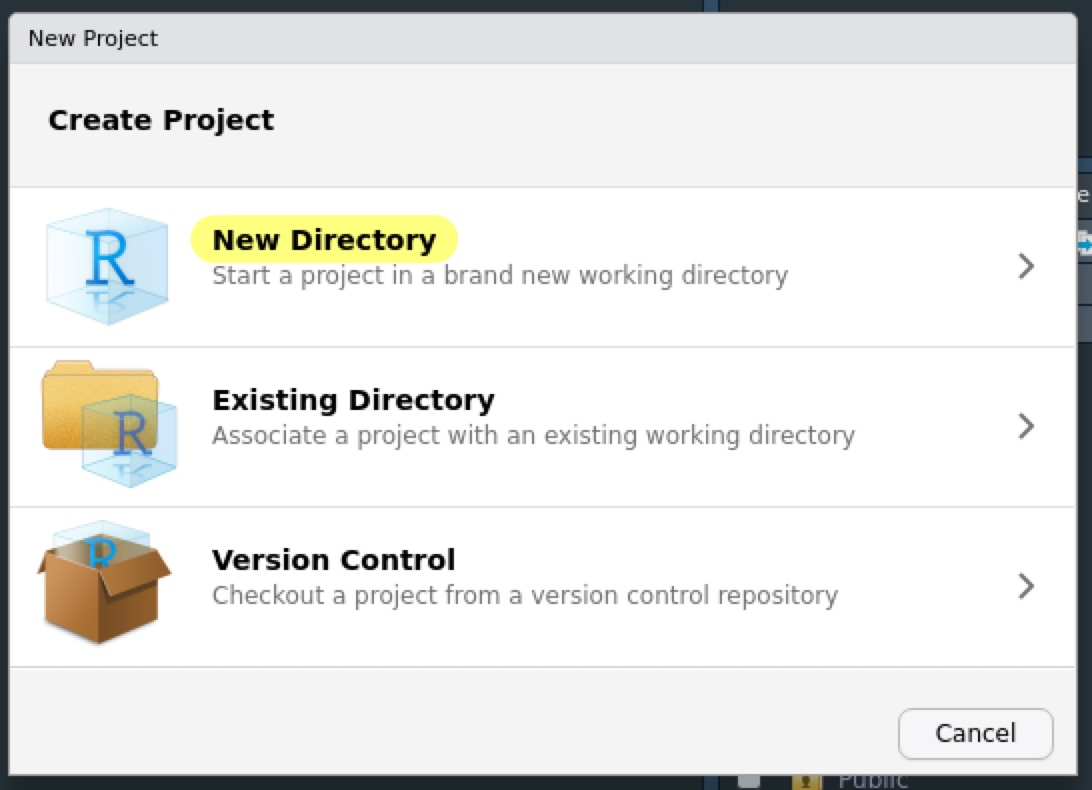
\includegraphics{figures/workflow3.jpg}

基本的には\texttt{New\ Project}を選択します。

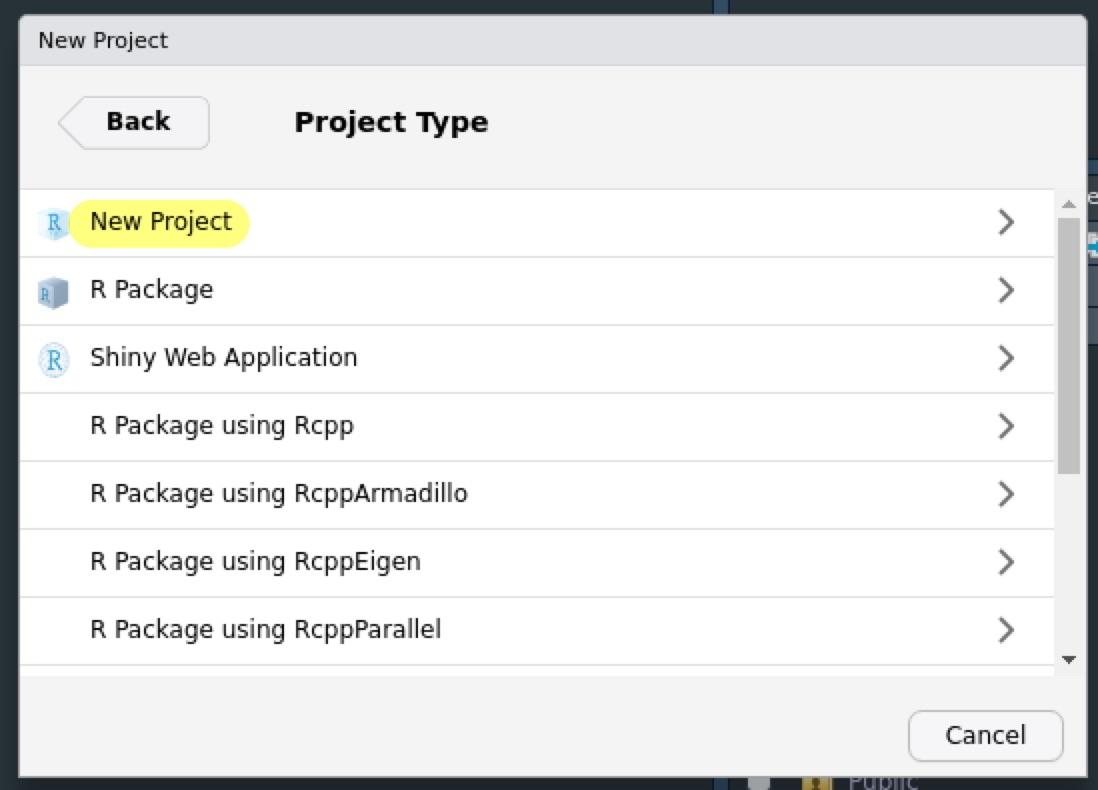
\includegraphics{figures/workflow4.jpg}

最後に、プロジェクト用のフォルダの名前とそのフォルダを置くフォルダのパスを指定して\texttt{Create\ Project}をクリックします。

\begin{itemize}
\tightlist
\item
  フォルダ名は必ず英数字と-や\_で書き、\textbf{日本語は避けましょう}。
\item
  既存のフォルダを使う場合はパスを指定するだけです。
\end{itemize}

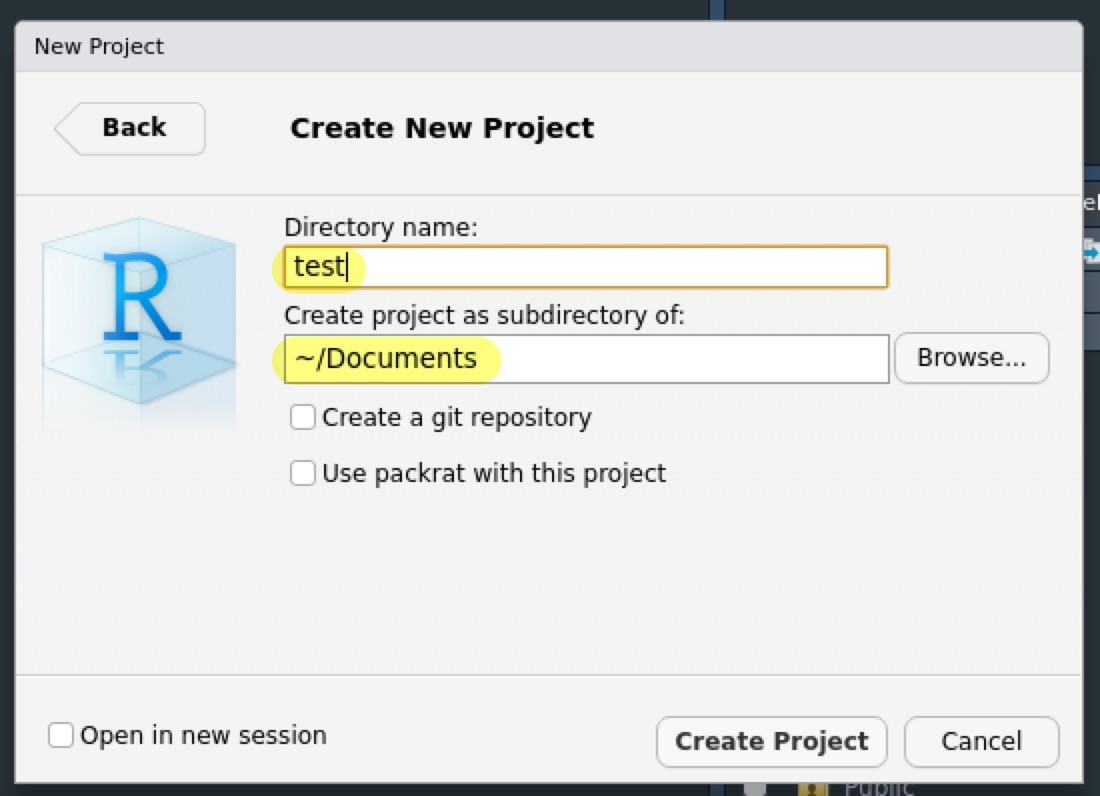
\includegraphics{figures/workflow5.jpg}

\begin{itemize}
\tightlist
\item
  例えば今回は\texttt{Documents}フォルダの中に\texttt{test}という名前のプロジェクトを作成しました。
\end{itemize}

一度、RStudioを終了し、先程指定したパス通りの場所にフォルダができていることを確認してください。
そのフォルダの中に、プロジェクト名と同じ名前の\texttt{.Rproj}ファイルができているはずです。

\hypertarget{ux30d7ux30edux30b8ux30a7ux30afux30c8ux306eux8d77ux52d5}{%
\paragraph{プロジェクトの起動}\label{ux30d7ux30edux30b8ux30a7ux30afux30c8ux306eux8d77ux52d5}}

それをダブルクリックしてみるとRStudioが起動されます。
このとき、すでに作業ディレクトリはプロジェクト用フォルダに指定されているのです。

\begin{itemize}
\tightlist
\item
  \texttt{getwd()}で作業ディレクトリを確認してみて下さい。
\end{itemize}

\hypertarget{ux30efux30fcux30afux30b9ux30daux30fcux30b9ux306eux4fddux5b58ux3068ux518dux958b}{%
\paragraph{ワークスペースの保存と再開*}\label{ux30efux30fcux30afux30b9ux30daux30fcux30b9ux306eux4fddux5b58ux3068ux518dux958b}}

どうしても一度分析を中断して、再開したい場合はワークスペースを保存しておきましょう。
上記画面で\texttt{Save\ workflow\ to\ .RData\ on\ exit}が\texttt{Ask}になっている場合、RStudioを終了する際にワークスペースを保存するのか聞かれるはずなので、保存します。

\begin{itemize}
\tightlist
\item
  ちなみに、\texttt{.RData}ファイルはRのワークスペース(の一部)を保存するデータ形式です。
\end{itemize}

すると、フォルダ内に\texttt{.RData}ファイルができるので、再開するときに\texttt{load()}に当該ファイルのパスを入力して実行するとワークスペースが復元されます。

\hypertarget{rstudioux306eux8a2dux5b9a}{%
\subsubsection{RStudioの設定*}\label{rstudioux306eux8a2dux5b9a}}

\hypertarget{rstudioux8d77ux52d5ux6642ux306eux6319ux52d5}{%
\paragraph{RStudio起動時の挙動}\label{rstudioux8d77ux52d5ux6642ux306eux6319ux52d5}}

\texttt{Tools\ \textgreater{}\ Global\ Options}を開き、\texttt{Genral}の中で以下のチェックを外します。

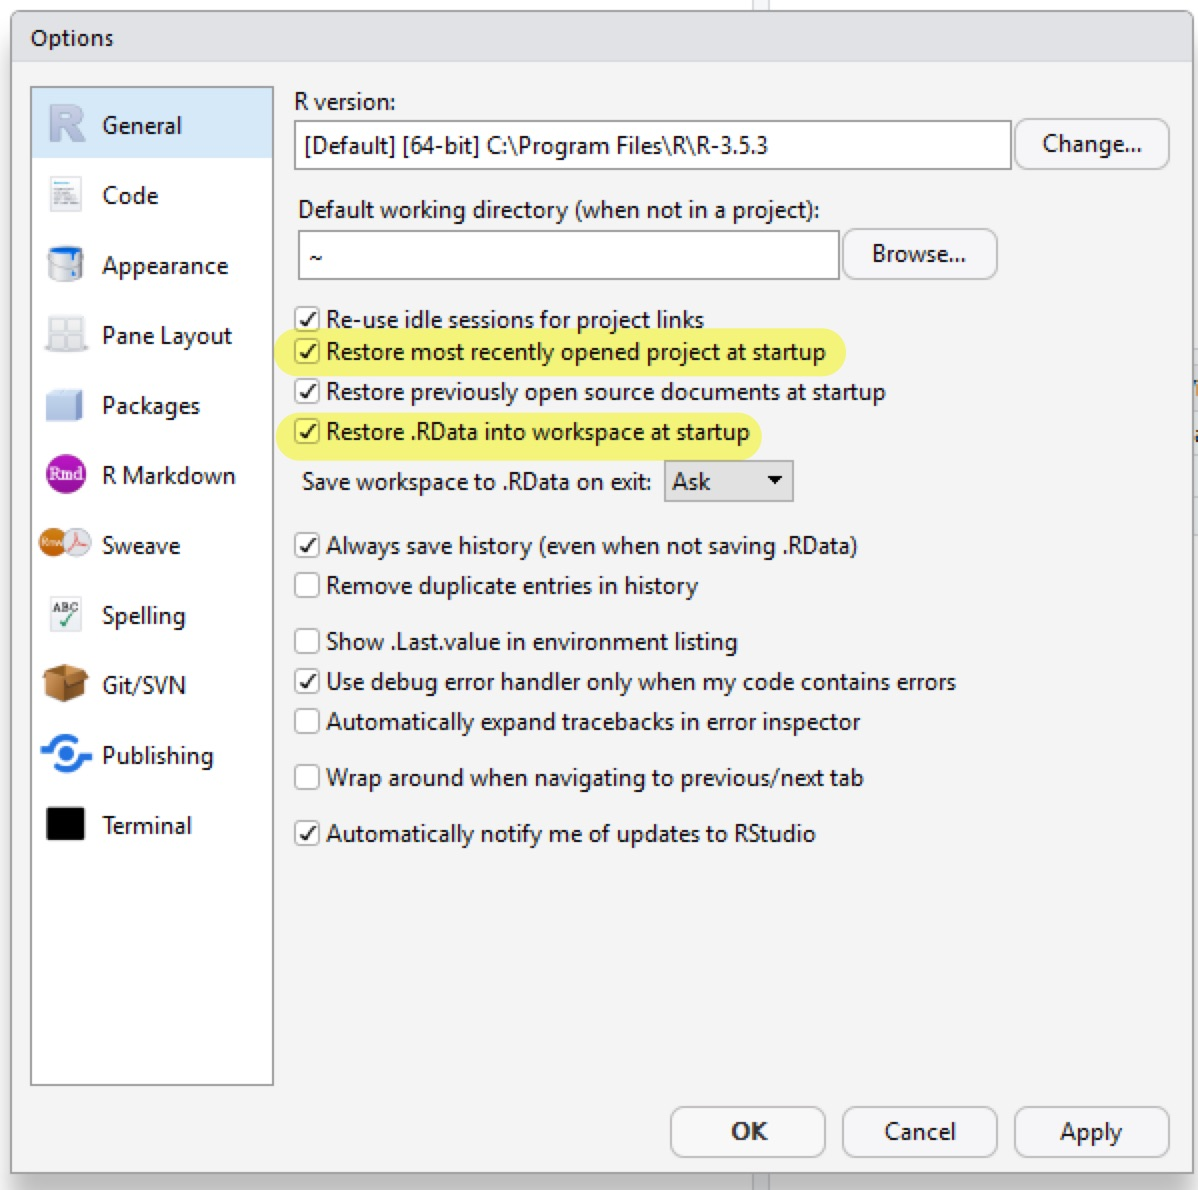
\includegraphics{figures/Rstudio4.jpg}

平たく言うとRStudioを起動したときに前回の続きが残っていない真っさらな状態にしておきます。

\hypertarget{ux6587ux5b57ux30b3ux30fcux30c9}{%
\paragraph{文字コード}\label{ux6587ux5b57ux30b3ux30fcux30c9}}

日本語がしばしば文字化けすることがあります。
なぜならWindowsではShift-JIS、LinuxとMacではUTF-8と呼ばれるエンコーディング(平たく言うとPCが文字を表示する方法)形式だからです。

\begin{itemize}
\tightlist
\item
  詳しくは\href{encoding-r.html}{Rにおける文字コード}を参照して下さい。
\end{itemize}

UTF-8が世界的に使われているので、\texttt{Code\ \textgreater{}\ Saving\ \textgreater{}\ Default\ text\ encoding}を\texttt{UTF-8}にしておきます。

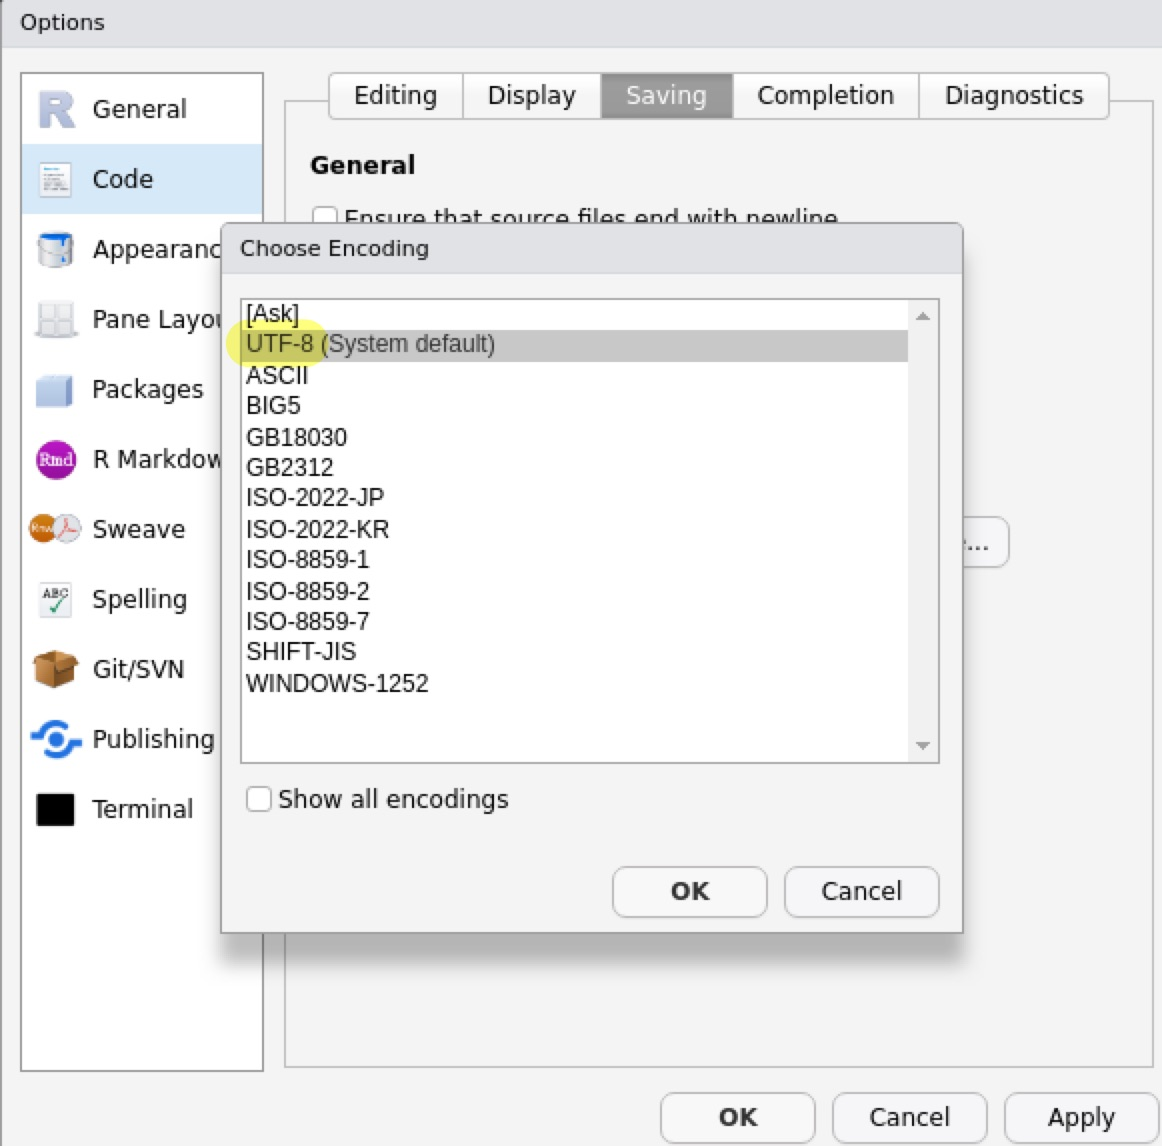
\includegraphics{figures/Rstudio7.jpg}

もし、日本語を含むファイルをRStudioで開いたときに文字化けしている場合、Windowsを使っている人はUTF-8のファイルをShift-JISで開いたということなので、\texttt{File\ \textgreater{}\ Reopen\ with\ Encoding}で\texttt{UTF-8}を選択します。

逆にMacの場合はShift-JISのファイルをUTF-8で開いているので同様に\texttt{Shift-JIS}で開きます。

\begin{itemize}
\tightlist
\item
  Windowsの人はUTF-8をデフォルトのエンコーディングにしてしまうといいでしょう。
\end{itemize}

\hypertarget{intro-r}{%
\section{Rプログラミング入門}\label{intro-r}}

Rによるプログラミングの基本として、

\begin{itemize}
\tightlist
\item
  \protect\hyperlink{ux30aaux30d6ux30b8ux30a7ux30afux30c8}{オブジェクト}
\item
  \protect\hyperlink{ux95a2ux6570}{関数}
\item
  \protect\hyperlink{ux30d1ux30c3ux30b1ux30fcux30b8}{パッケージ}
\end{itemize}

について解説します。

大雑把に言えば、Rではオブジェクトとしてデータを読み込み、関数によってオブジェクト(=データ)の処理や分析を行います。
パッケージによって様々な関数を追加することで、処理や分析の幅を広げます。

RStudioでは左(下)にコンソールが表示され、\texttt{\textgreater{}}の右側にコマンドを打ち込み、\texttt{Enter}を押すことで実行されます。

\begin{itemize}
\tightlist
\item
  本格的に分析する場合はRスクリプトを作成します。
\end{itemize}

\hypertarget{ux95a2ux6570}{%
\subsection{関数}\label{ux95a2ux6570}}

\textbf{関数} (function) とは何かを入力すると、何かを出力するものです。
例えば、

\begin{Shaded}
\begin{Highlighting}[]
\KeywordTok{print}\NormalTok{(}\StringTok{"Hello, World."}\NormalTok{)}
\end{Highlighting}
\end{Shaded}

\begin{verbatim}
## [1] "Hello, World."
\end{verbatim}

というコードは、\texttt{"Hello,\ World."}という文字列を\texttt{print()}という関数に入力し、その文字列を出力しています。

\begin{itemize}
\tightlist
\item
  Rでは、関数は\texttt{関数名()}という形を取ります。
\item
  入力するものを入力引数 (input argument) 、出力するものを出力引数 (output argument) と呼んだりします。
\end{itemize}

次のように、入力引数も出力引数も1つとは限りません。

\begin{Shaded}
\begin{Highlighting}[]
\KeywordTok{rnorm}\NormalTok{(}\DataTypeTok{n =} \DecValTok{10}\NormalTok{, }\DataTypeTok{mean =} \DecValTok{0}\NormalTok{, }\DataTypeTok{sd =} \DecValTok{1}\NormalTok{)}
\end{Highlighting}
\end{Shaded}

\begin{verbatim}
##  [1] -1.42452621 -0.42007188 -0.11354578  0.30189294 -0.29613240  0.37013165
##  [7]  0.02458299  0.95447871 -2.49405815 -0.35534634
\end{verbatim}

さて、この関数は何をしているのでしょうか。
Rでは、関数名の前に\texttt{?}をつけて実行することで、その関数のヘルプを見ることができます。

\begin{Shaded}
\begin{Highlighting}[]
\NormalTok{?rnorm}
\end{Highlighting}
\end{Shaded}

英語で関数の使い方が解説されていますが、\texttt{rnorm(n\ =\ 10,\ mean\ =\ 0,\ sd\ =\ 1)}は平均0、標準偏差1の(標準)正規分布に従う乱数を10個だけ生じさせています。

入力引数は\texttt{=}で明示的に指定する場合、どのような順番でも構いません。

\begin{Shaded}
\begin{Highlighting}[]
\KeywordTok{rnorm}\NormalTok{(}\DataTypeTok{mean =} \DecValTok{0}\NormalTok{, }\DataTypeTok{sd =} \DecValTok{1}\NormalTok{, }\DataTypeTok{n =} \DecValTok{10}\NormalTok{)}
\end{Highlighting}
\end{Shaded}

入力引数を明示的に指定しない場合、ヘルプにある順番で入力します。
以下の例は上述のものと同じです。

\begin{Shaded}
\begin{Highlighting}[]
\KeywordTok{rnorm}\NormalTok{(}\DecValTok{10}\NormalTok{, }\DecValTok{0}\NormalTok{, }\DecValTok{1}\NormalTok{)}
\end{Highlighting}
\end{Shaded}

また、ヘルプで\texttt{mean\ =\ 0,\ sd\ =\ 1}のように書かれている場合、デフォルトが定められています。
実行者が入力引数を指定しない限り、デフォルト値が使用されます。
したがって、以下の例もこれまでと同じコードです。

\begin{Shaded}
\begin{Highlighting}[]
\KeywordTok{rnorm}\NormalTok{(}\DecValTok{10}\NormalTok{)}
\end{Highlighting}
\end{Shaded}

\hypertarget{ux7dcfux79f0ux95a2ux6570}{%
\subsubsection{総称関数*}\label{ux7dcfux79f0ux95a2ux6570}}

総称関数 (generic function) とは、Rにおいて入力引数の種類に応じて挙動が変わる関数のことを指します。
例えば、\texttt{summary()}という関数はデータフレームが入力引数の場合には記述統計を表示しますが、回帰分析の結果の場合は回帰表を出力します。

総称関数のヘルプを見る場合は、以下のように、関数名に\texttt{.}をつけて入力引数の種類を書きます。

\begin{Shaded}
\begin{Highlighting}[]
\NormalTok{?summary.data.frame}
\NormalTok{?summary.lm}
\end{Highlighting}
\end{Shaded}

\hypertarget{ux30aaux30d6ux30b8ux30a7ux30afux30c8}{%
\subsection{オブジェクト}\label{ux30aaux30d6ux30b8ux30a7ux30afux30c8}}

Rでは\texttt{\textless{}-}でオブジェクトを作成することができます。
例えば、20個の正規分布に従う乱数を\texttt{x}という名前のオブジェクトとして作成します。

\begin{Shaded}
\begin{Highlighting}[]
\NormalTok{x <-}\StringTok{ }\KeywordTok{rnorm}\NormalTok{(}\DecValTok{20}\NormalTok{)}
\end{Highlighting}
\end{Shaded}

\begin{itemize}
\tightlist
\item
  RStudioでは\texttt{\textless{}-}はショートカット\texttt{Alt\ +\ -}で入力できます。
\end{itemize}

実際に、乱数が\texttt{x}に格納されていることが分かります。

\begin{Shaded}
\begin{Highlighting}[]
\NormalTok{x}
\end{Highlighting}
\end{Shaded}

\begin{verbatim}
##  [1] -1.1242721  1.3335992  1.9714474  0.6266777  1.8654255  1.8993201
##  [7]  0.8408928  0.8390228 -0.2873750  0.5132134 -1.0851594  0.5637831
## [13] -0.3414139 -0.6298208  0.6594867 -0.6565816 -1.0344331 -0.2830303
## [19] -0.7212691  0.4840311
\end{verbatim}

RStudioの場合、右上の\texttt{Environment}パネルに生成されたオブジェクトが表示されます。

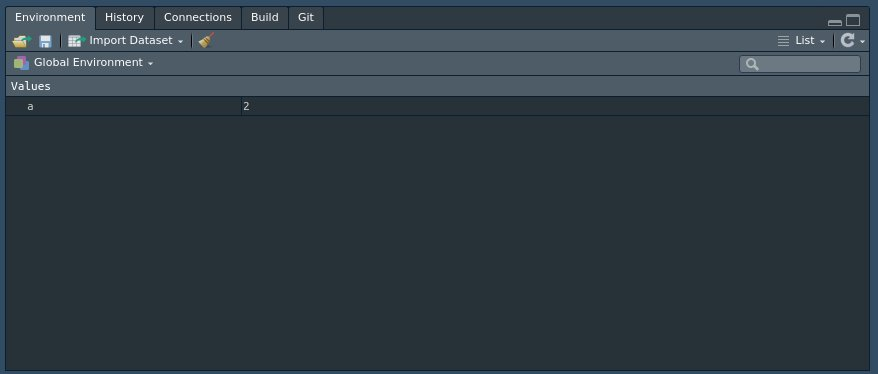
\includegraphics{figures/intro_r1.jpg}

オブジェクトを入力引数とすることも可能です。
\texttt{x}の平均と標準偏差を求めてみます。

\begin{Shaded}
\begin{Highlighting}[]
\KeywordTok{mean}\NormalTok{(x)}
\end{Highlighting}
\end{Shaded}

\begin{verbatim}
## [1] 0.2716772
\end{verbatim}

\begin{Shaded}
\begin{Highlighting}[]
\KeywordTok{sd}\NormalTok{(x)}
\end{Highlighting}
\end{Shaded}

\begin{verbatim}
## [1] 1.012273
\end{verbatim}

もちろん、出力引数を新しいオブジェクトにすることもできます。

\begin{Shaded}
\begin{Highlighting}[]
\NormalTok{x.mean <-}\StringTok{ }\KeywordTok{mean}\NormalTok{(x)}
\NormalTok{x.mean}
\end{Highlighting}
\end{Shaded}

\begin{verbatim}
## [1] 0.2716772
\end{verbatim}

\begin{itemize}
\tightlist
\item
  オブジェクトの名前にはアルファベットと数字、\texttt{.}と\texttt{\_}が使えます。
\item
  ただし、数字は最初の文字としては使えません。
\end{itemize}

オブジェクトは上書きすることもできます。

\begin{Shaded}
\begin{Highlighting}[]
\NormalTok{x.mean <-}\StringTok{ }\KeywordTok{mean}\NormalTok{(}\KeywordTok{rnorm}\NormalTok{(}\DecValTok{20}\NormalTok{))}
\NormalTok{x.mean}
\end{Highlighting}
\end{Shaded}

\begin{verbatim}
## [1] 0.428162
\end{verbatim}

\begin{itemize}
\tightlist
\item
  先ほどとは違う値に上書きされていることが分かります。
\end{itemize}

\hypertarget{ux30d1ux30c3ux30b1ux30fcux30b8}{%
\subsection{パッケージ}\label{ux30d1ux30c3ux30b1ux30fcux30b8}}

大雑把に言って、Rによるデータ分析は\textbf{データをオブジェクトとして読み込み、いろいろな関数で処理を行うこと}で実行します。

つまり、関数が重要なのですが、Rで標準に備わっている関数には限界があります。
そこで、様々な研究者が関数を作成し、それをまとめたものを\textbf{パッケージ}として公開しています。

\begin{itemize}
\tightlist
\item
  基本的に、\href{https://cran.r-project.org/}{CRAN}でパッケージは公開されます。
\item
  ライブラリやモジュールと呼んだりすることもあります。
\end{itemize}

\hypertarget{cranux304bux3089ux306eux30a4ux30f3ux30b9ux30c8ux30fcux30eb}{%
\subsubsection{CRANからのインストール}\label{cranux304bux3089ux306eux30a4ux30f3ux30b9ux30c8ux30fcux30eb}}

パッケージをインストールするには、\texttt{install.packages()}という関数にパッケージ名を入れて実行します。
試しに、\href{https://www.tidyverse.org/}{Tidyverse}という幅広く使われているパッケージをインストールしてみます。

\begin{Shaded}
\begin{Highlighting}[]
\KeywordTok{install.packages}\NormalTok{(}\StringTok{"tidyverse"}\NormalTok{)}
\end{Highlighting}
\end{Shaded}

\texttt{"}でパッケージ名を囲まないとエラーになります。

\begin{Shaded}
\begin{Highlighting}[]
\KeywordTok{install.packages}\NormalTok{(tidyverse)}
\end{Highlighting}
\end{Shaded}

\begin{verbatim}
## Error in install.packages(tidyverse): object 'tidyverse' not found
\end{verbatim}

RStudioの場合、\texttt{Packages}パネル(デフォルトの場合は右下)の中に\texttt{Install}というボタンがあり、

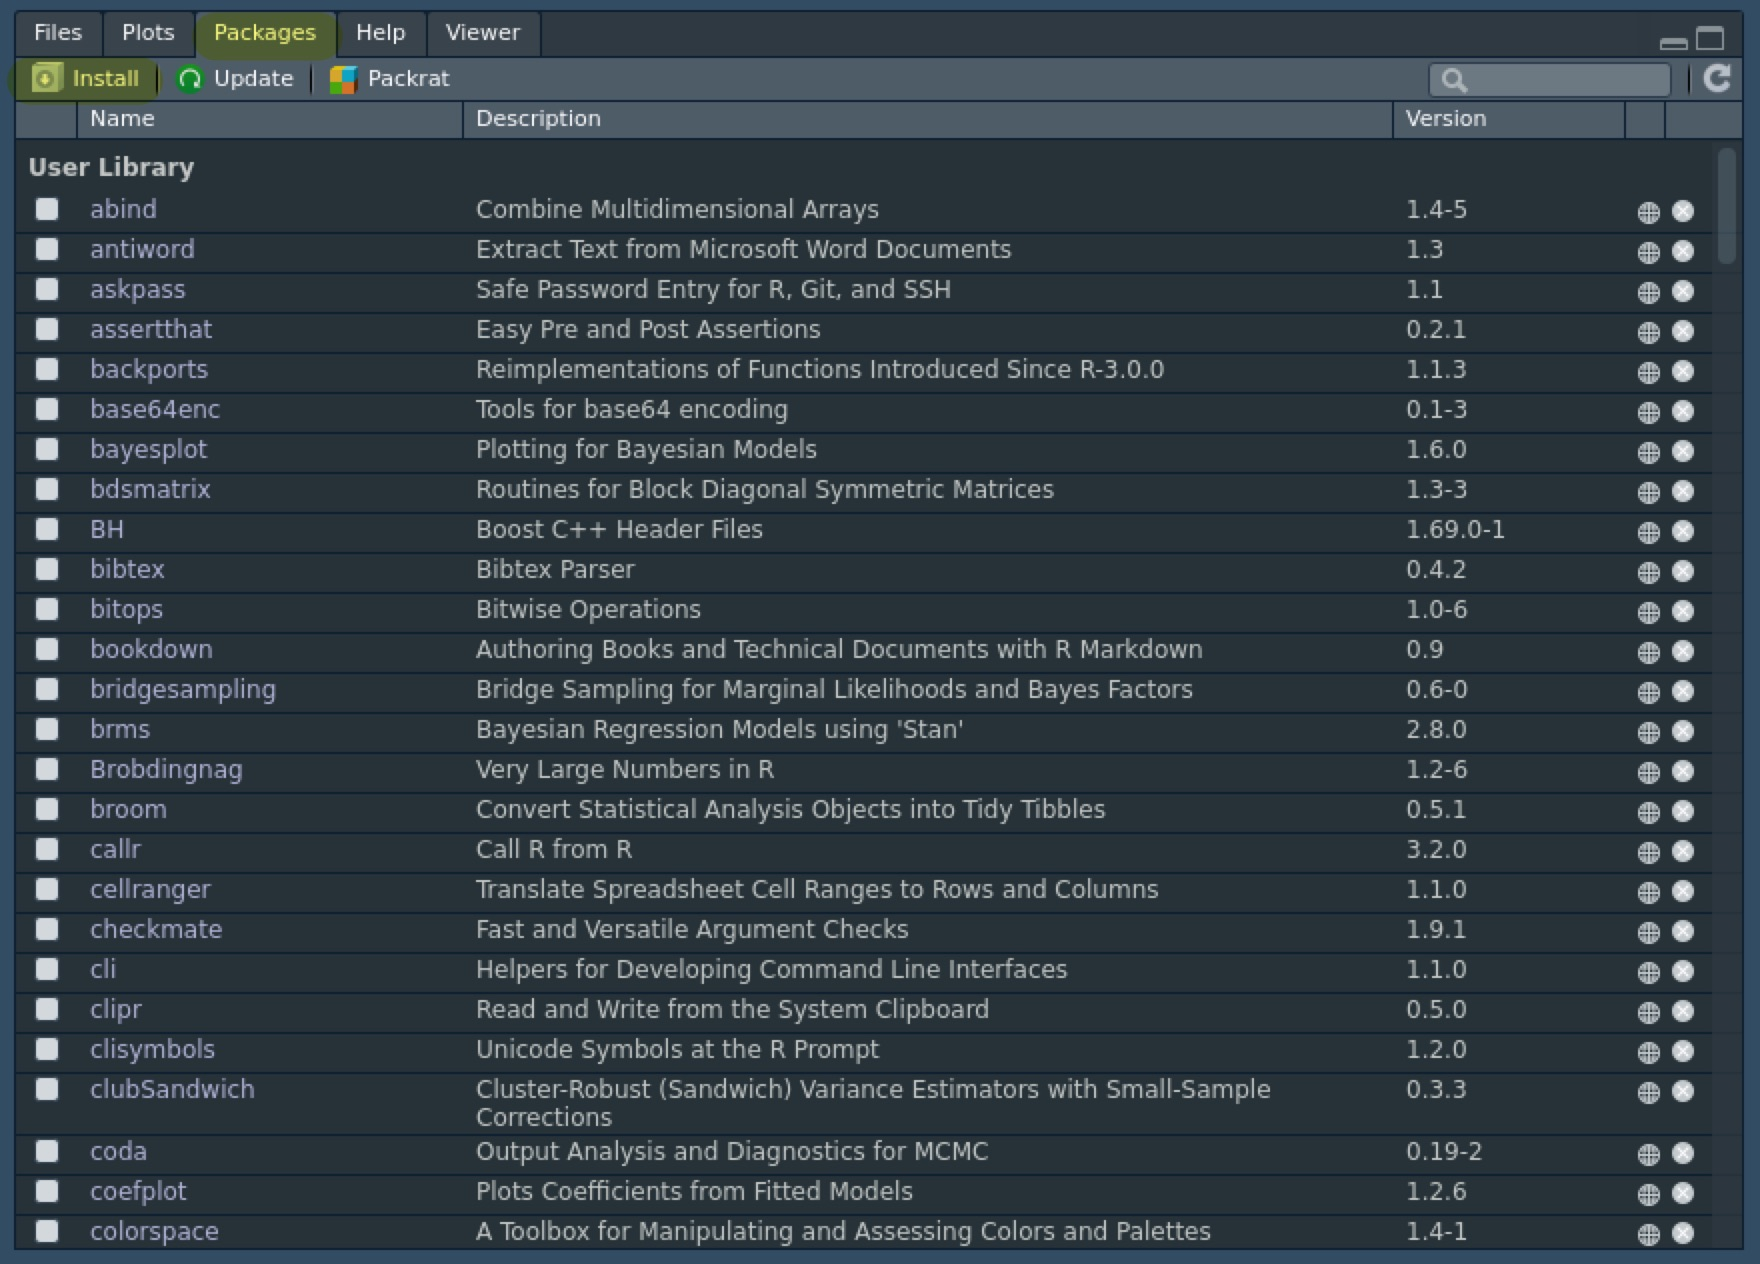
\includegraphics{figures/intro_r2.jpg}

そこにパッケージ名を入力してインストールすることも可能です。

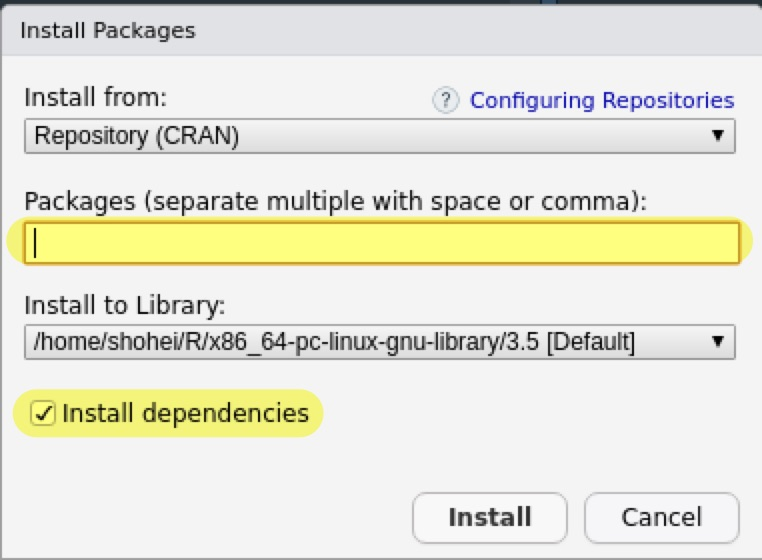
\includegraphics{figures/intro_r3.jpg}

インストールしたパッケージに対して再び\texttt{install.packages()}を行うと、最新版にアップデートされます。

\begin{itemize}
\tightlist
\item
  RStudioの場合、\texttt{Packages}パネルに\texttt{Update}というボタンがあり、アップデートできるパッケージを自動検索してくれます。
\end{itemize}

\hypertarget{githubux304bux3089ux306eux30a4ux30f3ux30b9ux30c8ux30fcux30eb}{%
\subsubsection{GitHubからのインストール*}\label{githubux304bux3089ux306eux30a4ux30f3ux30b9ux30c8ux30fcux30eb}}

パッケージの開発版や一部のパッケージは\href{https://github.com/}{GitHub}上で公開されています。

GitHub上のパッケージをインストールする場合は\texttt{devtools}というパッケージを使うので、まずはインストールと読み込みを行います。

\begin{Shaded}
\begin{Highlighting}[]
\KeywordTok{install.packages}\NormalTok{(}\StringTok{"devtools"}\NormalTok{)}
\KeywordTok{library}\NormalTok{(devtools)}
\end{Highlighting}
\end{Shaded}

インストールには\texttt{install\_github()}を使いますが、入力はパッケージ名ではなく\texttt{ユーザー名/レポジトリ名}となる点に注意してください。

\hypertarget{ux30d1ux30c3ux30b1ux30fcux30b8ux306eux8aadux307fux8fbcux307f}{%
\subsubsection{パッケージの読み込み}\label{ux30d1ux30c3ux30b1ux30fcux30b8ux306eux8aadux307fux8fbcux307f}}

パッケージはインストールしただけでは使用することはできず、\texttt{library()}で読み込む必要があります。

\begin{Shaded}
\begin{Highlighting}[]
\KeywordTok{library}\NormalTok{(tidyverse)}
\end{Highlighting}
\end{Shaded}

\begin{itemize}
\tightlist
\item
  この場合は\texttt{"}で囲む必要はありません。
\item
  インストールは一回で十分です。
\end{itemize}

RStudioであれば\texttt{Packages}パネルにインストール済みのパッケージ一覧があるので、パッケージ名をクリックすると含まれる関数一覧を見ることができます。

\begin{itemize}
\tightlist
\item
  同様のものは\href{https://cran.r-project.org/}{CRAN}でも\texttt{pdf}形式で見ることができます。
\item
  一部のソフトウェアは\href{https://www.jstatsoft.org/index}{Journal of Statistical Software}などで論文が公開されています。
\end{itemize}

\hypertarget{tidyverseux3068ux306f}{%
\subsubsection{\texorpdfstring{\texttt{tidyverse}とは*}{tidyverseとは*}}\label{tidyverseux3068ux306f}}

Tidyverseとは広義にはRにおけるデータ処理を行うためのパッケージを開発するプロジェクトであり、狭義にはそこで開発されたパッケージの一部を指します。
具体的には、

\begin{itemize}
\tightlist
\item
  \texttt{ggplot2}
\item
  \texttt{dplyr}
\item
  \texttt{tidyr}
\item
  \texttt{readr}
\item
  \texttt{purrr}
\item
  \texttt{tibble}
\item
  \texttt{stringr}
\item
  \texttt{forcats}
\end{itemize}

になります。

パッケージとしての\texttt{tidyverse}を読み込むことで、上記のパッケージを読み込んでいます。

なお、プロジェクト全体としては、上記のもの以外にも多くのパッケージが開発されています。

\hypertarget{inter-r}{%
\section{Rプログラミング応用*}\label{inter-r}}

Rによる、より高度な作業のために

\begin{itemize}
\tightlist
\item
  代表的な\protect\hyperlink{ux30aaux30d6ux30b8ux30a7ux30afux30c8ux306eux30afux30e9ux30b9}{オブジェクトのクラス}
\item
  オリジナルの\protect\hyperlink{ux95a2ux6570ux306eux4f5cux6210}{関数の作成}
\item
  \protect\hyperlink{ux30ebux30fcux30d7}{ループ}や\protect\hyperlink{ux6761ux4ef6ux5206ux5c90}{条件分岐}
\end{itemize}

などを学びます。

\hypertarget{ux30aaux30d6ux30b8ux30a7ux30afux30c8ux306eux30afux30e9ux30b9}{%
\subsection{オブジェクトのクラス}\label{ux30aaux30d6ux30b8ux30a7ux30afux30c8ux306eux30afux30e9ux30b9}}

オブジェクトの種類を\textbf{クラス}と呼びます。
\texttt{class()}にオブジェクトを入力するとクラスが分かります。

最も使われるのは数値 ()numeric, real) です。

\begin{Shaded}
\begin{Highlighting}[]
\KeywordTok{class}\NormalTok{(}\DecValTok{1}\NormalTok{)}
\end{Highlighting}
\end{Shaded}

\begin{verbatim}
## [1] "numeric"
\end{verbatim}

厳密には数値と整数 (integer) は異なりますが、気にしないといけない局面は少ないと思います。

\begin{Shaded}
\begin{Highlighting}[]
\KeywordTok{class}\NormalTok{(2L)}
\end{Highlighting}
\end{Shaded}

\begin{verbatim}
## [1] "integer"
\end{verbatim}

他には、文字列 (character) や

\begin{Shaded}
\begin{Highlighting}[]
\KeywordTok{class}\NormalTok{(}\StringTok{"Hello, World."}\NormalTok{)}
\end{Highlighting}
\end{Shaded}

\begin{verbatim}
## [1] "character"
\end{verbatim}

論理値 (logical) などもあります。

\begin{Shaded}
\begin{Highlighting}[]
\KeywordTok{class}\NormalTok{(}\OtherTok{TRUE}\NormalTok{)}
\end{Highlighting}
\end{Shaded}

\begin{verbatim}
## [1] "logical"
\end{verbatim}

論理値は主に条件式が満たされるかどうかを示します。

\begin{Shaded}
\begin{Highlighting}[]
\DecValTok{1} \OperatorTok{==}\StringTok{ }\DecValTok{1}
\end{Highlighting}
\end{Shaded}

\begin{verbatim}
## [1] TRUE
\end{verbatim}

\begin{Shaded}
\begin{Highlighting}[]
\DecValTok{0} \OperatorTok{>}\StringTok{ }\DecValTok{2}
\end{Highlighting}
\end{Shaded}

\begin{verbatim}
## [1] FALSE
\end{verbatim}

ちなみに、\texttt{TRUE}は数値としての\texttt{1}、\texttt{FALSE}は\texttt{0}にもなります。

\begin{Shaded}
\begin{Highlighting}[]
\OtherTok{TRUE} \OperatorTok{+}\StringTok{ }\DecValTok{1}
\end{Highlighting}
\end{Shaded}

\begin{verbatim}
## [1] 2
\end{verbatim}

\begin{Shaded}
\begin{Highlighting}[]
\OtherTok{FALSE} \OperatorTok{*}\StringTok{ }\DecValTok{2}
\end{Highlighting}
\end{Shaded}

\begin{verbatim}
## [1] 0
\end{verbatim}

また、因子型 (factor) と呼ばれるクラスもあります。
カテゴリカル変数と言ったほうが分かりやすいかもしれません。

\begin{Shaded}
\begin{Highlighting}[]
\NormalTok{x <-}\StringTok{ }\KeywordTok{factor}\NormalTok{(}\DecValTok{1}\NormalTok{)}
\NormalTok{x}
\end{Highlighting}
\end{Shaded}

\begin{verbatim}
## [1] 1
## Levels: 1
\end{verbatim}

\begin{Shaded}
\begin{Highlighting}[]
\KeywordTok{class}\NormalTok{(x)}
\end{Highlighting}
\end{Shaded}

\begin{verbatim}
## [1] "factor"
\end{verbatim}

\texttt{X}の中身は\texttt{1}ですが、数値ではなくカテゴリーになっているので、数値として操作することはできません。

\begin{Shaded}
\begin{Highlighting}[]
\NormalTok{x }\OperatorTok{+}\StringTok{ }\DecValTok{1}
\end{Highlighting}
\end{Shaded}

\begin{verbatim}
## Warning in Ops.factor(x, 1): '+' not meaningful for factors
\end{verbatim}

\begin{verbatim}
## [1] NA
\end{verbatim}

Rではベクトルには特別なクラスは付与されていません。
ベクトルは\texttt{c()}に中身を入力して作成します。

\begin{Shaded}
\begin{Highlighting}[]
\NormalTok{x <-}\StringTok{ }\KeywordTok{c}\NormalTok{(}\DecValTok{1}\NormalTok{,}\DecValTok{3}\NormalTok{,}\DecValTok{5}\NormalTok{)}
\NormalTok{x}
\end{Highlighting}
\end{Shaded}

\begin{verbatim}
## [1] 1 3 5
\end{verbatim}

行列 (matrix) はクラスとして存在します。

\begin{Shaded}
\begin{Highlighting}[]
\NormalTok{x <-}\StringTok{ }\KeywordTok{matrix}\NormalTok{(}\KeywordTok{c}\NormalTok{(}\DecValTok{1}\NormalTok{,}\DecValTok{3}\NormalTok{,}\DecValTok{5}\NormalTok{,}\DecValTok{7}\NormalTok{), }\DecValTok{2}\NormalTok{, }\DecValTok{2}\NormalTok{)}
\NormalTok{x}
\end{Highlighting}
\end{Shaded}

\begin{verbatim}
##      [,1] [,2]
## [1,]    1    5
## [2,]    3    7
\end{verbatim}

\begin{Shaded}
\begin{Highlighting}[]
\KeywordTok{class}\NormalTok{(x)}
\end{Highlighting}
\end{Shaded}

\begin{verbatim}
## [1] "matrix"
\end{verbatim}

他に、データフレーム (data.frame) やリスト (list) などもあります。

クラスを確認するときは、\texttt{is.*()}の形をとる関数を使います。

\begin{Shaded}
\begin{Highlighting}[]
\KeywordTok{is.numeric}\NormalTok{(}\DecValTok{1}\NormalTok{)}
\end{Highlighting}
\end{Shaded}

\begin{verbatim}
## [1] TRUE
\end{verbatim}

\begin{Shaded}
\begin{Highlighting}[]
\KeywordTok{is.character}\NormalTok{(}\DecValTok{1}\NormalTok{)}
\end{Highlighting}
\end{Shaded}

\begin{verbatim}
## [1] FALSE
\end{verbatim}

クラスを変更するときは、\texttt{as.*()}のような関数を使います。

\begin{Shaded}
\begin{Highlighting}[]
\KeywordTok{as.factor}\NormalTok{(}\DecValTok{1}\NormalTok{)}
\end{Highlighting}
\end{Shaded}

\begin{verbatim}
## [1] 1
## Levels: 1
\end{verbatim}

\begin{Shaded}
\begin{Highlighting}[]
\KeywordTok{as.character}\NormalTok{(}\DecValTok{1}\NormalTok{)}
\end{Highlighting}
\end{Shaded}

\begin{verbatim}
## [1] "1"
\end{verbatim}

\begin{itemize}
\tightlist
\item
  必ずしも全てのクラスが任意のクラスに変換できるわけではありません(例えば、文字列から数値など)。
\end{itemize}

\hypertarget{ux95a2ux6570ux306eux4f5cux6210}{%
\subsection{関数の作成}\label{ux95a2ux6570ux306eux4f5cux6210}}

Rで関数を自作する際は\texttt{function()\{\}}という関数を使います。

\begin{itemize}
\tightlist
\item
  \texttt{()}の中に入力引数を記述します。
\item
  \texttt{\{\}}の中に処理内容を記述し、最後に\texttt{return()}で出力引数を指定します。
\end{itemize}

例えば、数値ベクトルを入力引数として、平均と標準偏差を出力引数とする関数を作成します。

\begin{Shaded}
\begin{Highlighting}[]
\NormalTok{mean_sd <-}\StringTok{ }\ControlFlowTok{function}\NormalTok{(x) \{ }\CommentTok{# 入力引数の名前をxとしておきます。}
\NormalTok{  mean.x <-}\StringTok{ }\KeywordTok{mean}\NormalTok{(x) }\CommentTok{# 平均を計算します。}
\NormalTok{  sd.x <-}\StringTok{ }\KeywordTok{sd}\NormalTok{(x) }\CommentTok{# 標準偏差を計算します。}
  \KeywordTok{return}\NormalTok{(}\KeywordTok{c}\NormalTok{(mean.x, sd.x)) }\CommentTok{# 出力引数を指定します。}
\NormalTok{\}}
\end{Highlighting}
\end{Shaded}

実際に実行してみます。

\begin{Shaded}
\begin{Highlighting}[]
\NormalTok{x <-}\StringTok{ }\KeywordTok{rnorm}\NormalTok{(}\DecValTok{100}\NormalTok{)}
\KeywordTok{mean_sd}\NormalTok{(x)}
\end{Highlighting}
\end{Shaded}

\begin{verbatim}
## [1] -0.04230494  1.00539856
\end{verbatim}

\hypertarget{ux30ebux30fcux30d7}{%
\subsection{ループ}\label{ux30ebux30fcux30d7}}

\textbf{ループ}とは同一の処理を複数回実行することを指します。
例えば、100個の標準正規分布に従う乱数の平均を5回求める処理は次のようになります。

\begin{Shaded}
\begin{Highlighting}[]
\ControlFlowTok{for}\NormalTok{ (i }\ControlFlowTok{in} \DecValTok{1}\OperatorTok{:}\DecValTok{5}\NormalTok{) \{}
  \KeywordTok{print}\NormalTok{(}\KeywordTok{mean}\NormalTok{(}\KeywordTok{rnorm}\NormalTok{(}\DecValTok{100}\NormalTok{)))}
\NormalTok{\}}
\end{Highlighting}
\end{Shaded}

\begin{verbatim}
## [1] 0.1260475
## [1] -0.01005321
## [1] 0.0575182
## [1] -0.01412347
## [1] -0.06033713
\end{verbatim}

\texttt{for}ループとは\texttt{()}の中の\texttt{in}のあとのベクトルの第1要素から順番に\texttt{i}に代入して繰り返しています。
そのことは、次の例から解ると思います。

\begin{Shaded}
\begin{Highlighting}[]
\KeywordTok{head}\NormalTok{(letters)}
\end{Highlighting}
\end{Shaded}

\begin{verbatim}
## [1] "a" "b" "c" "d" "e" "f"
\end{verbatim}

\begin{itemize}
\tightlist
\item
  \texttt{letters}とはアルファベットのベクトルです。
\end{itemize}

\begin{Shaded}
\begin{Highlighting}[]
\ControlFlowTok{for}\NormalTok{ (i }\ControlFlowTok{in} \KeywordTok{head}\NormalTok{(letters)) \{}
  \KeywordTok{print}\NormalTok{(i)}
\NormalTok{\}}
\end{Highlighting}
\end{Shaded}

\begin{verbatim}
## [1] "a"
## [1] "b"
## [1] "c"
## [1] "d"
## [1] "e"
## [1] "f"
\end{verbatim}

\begin{itemize}
\tightlist
\item
  \texttt{for}ループとは別に、特定の条件が満たされるまで繰り返される\texttt{while}ループもあります。
\end{itemize}

ループ処理の結果を格納するには少しテクニックが必要です。
100個の乱数の平均を5回取ったものを\texttt{x}として保存したいとします。

まず、\texttt{x}を\texttt{NULL}オブジェクトとして作成します。

\begin{Shaded}
\begin{Highlighting}[]
\NormalTok{x <-}\StringTok{ }\OtherTok{NULL}
\NormalTok{x}
\end{Highlighting}
\end{Shaded}

\begin{verbatim}
## NULL
\end{verbatim}

\begin{itemize}
\tightlist
\item
  \texttt{NULL}とは空っぽのオブジェクト(0という数値や空白という文字ではない)です。
\end{itemize}

先程のループ処理の中で、計算した平均を\texttt{c()}で\texttt{x}にくっつけていきます。

\begin{Shaded}
\begin{Highlighting}[]
\ControlFlowTok{for}\NormalTok{ (i }\ControlFlowTok{in} \DecValTok{1}\OperatorTok{:}\DecValTok{5}\NormalTok{) \{}
\NormalTok{  x <-}\StringTok{ }\KeywordTok{c}\NormalTok{(x, }\KeywordTok{mean}\NormalTok{(}\KeywordTok{rnorm}\NormalTok{(}\DecValTok{100}\NormalTok{)))}
\NormalTok{\}}
\NormalTok{x}
\end{Highlighting}
\end{Shaded}

\begin{verbatim}
## [1] -0.01254183 -0.01507656 -0.04814641  0.08880067  0.05525210
\end{verbatim}

無事、5個の平均値が\texttt{x}に保存されていることがわかります。

実際に\texttt{for}ループの中で何が起こっているかは、次のコードで解ると思います。

\begin{Shaded}
\begin{Highlighting}[]
\NormalTok{x <-}\StringTok{ }\OtherTok{NULL}
\ControlFlowTok{for}\NormalTok{ (i }\ControlFlowTok{in} \DecValTok{1}\OperatorTok{:}\DecValTok{5}\NormalTok{) \{}
\NormalTok{  x <-}\StringTok{ }\KeywordTok{c}\NormalTok{(x, }\KeywordTok{mean}\NormalTok{(}\KeywordTok{rnorm}\NormalTok{(}\DecValTok{100}\NormalTok{)))}
  \KeywordTok{print}\NormalTok{(x)}
\NormalTok{\}}
\end{Highlighting}
\end{Shaded}

\begin{verbatim}
## [1] -0.08562251
## [1] -0.085622505  0.005231885
## [1] -0.085622505  0.005231885 -0.121550919
## [1] -0.085622505  0.005231885 -0.121550919  0.054285805
## [1] -0.085622505  0.005231885 -0.121550919  0.054285805  0.074869545
\end{verbatim}

\begin{itemize}
\tightlist
\item
  ループが一周するたびに、前回の\texttt{x}に新しい要素が付け加わり、新しい\texttt{x}として保存されています。
\end{itemize}

\texttt{NULL}オブジェクトを使ったループ結果の保存でよくあるミスは、やり直す際に\texttt{NULL}でリセットするのを忘れることです。
例えば、同じコードをもう一度実行しましょう。

\begin{Shaded}
\begin{Highlighting}[]
\ControlFlowTok{for}\NormalTok{ (i }\ControlFlowTok{in} \DecValTok{1}\OperatorTok{:}\DecValTok{5}\NormalTok{) \{}
\NormalTok{  x <-}\StringTok{ }\KeywordTok{c}\NormalTok{(x, }\KeywordTok{mean}\NormalTok{(}\KeywordTok{rnorm}\NormalTok{(}\DecValTok{100}\NormalTok{)))}
\NormalTok{\}}
\NormalTok{x}
\end{Highlighting}
\end{Shaded}

\begin{verbatim}
##  [1] -0.085622505  0.005231885 -0.121550919  0.054285805  0.074869545
##  [6]  0.016440166  0.108694760 -0.003228409  0.030114880  0.133772951
\end{verbatim}

\begin{itemize}
\tightlist
\item
  \texttt{x}に10個の平均値が入っています。
\end{itemize}

このようなミスを避ける方法の一つは、全体を関数として作成することです。

\begin{Shaded}
\begin{Highlighting}[]
\NormalTok{multi_mean <-}\StringTok{ }\ControlFlowTok{function}\NormalTok{() \{}
\NormalTok{  x <-}\StringTok{ }\OtherTok{NULL}
  \ControlFlowTok{for}\NormalTok{ (i }\ControlFlowTok{in} \DecValTok{1}\OperatorTok{:}\DecValTok{5}\NormalTok{) \{}
\NormalTok{    x <-}\StringTok{ }\KeywordTok{c}\NormalTok{(x, }\KeywordTok{mean}\NormalTok{(}\KeywordTok{rnorm}\NormalTok{(}\DecValTok{100}\NormalTok{)))}
\NormalTok{  \}}
  \KeywordTok{return}\NormalTok{(x)}
\NormalTok{\}}
\NormalTok{x <-}\StringTok{ }\KeywordTok{multi_mean}\NormalTok{()}
\NormalTok{x}
\end{Highlighting}
\end{Shaded}

\begin{verbatim}
## [1]  0.03679536 -0.02348755  0.01728398  0.13719900 -0.01580726
\end{verbatim}

\hypertarget{ux6761ux4ef6ux5206ux5c90}{%
\subsection{条件分岐}\label{ux6761ux4ef6ux5206ux5c90}}

\textbf{条件分岐}とは、特定の条件の場合に特定の動作を行うようにすることです。
例えば、正の場合\texttt{positive}、負の場合\texttt{negative}と出力するコマンドは次のようになります。

\begin{Shaded}
\begin{Highlighting}[]
\NormalTok{x <-}\StringTok{ }\KeywordTok{rnorm}\NormalTok{(}\DecValTok{1}\NormalTok{)}
\ControlFlowTok{if}\NormalTok{ (x }\OperatorTok{>}\StringTok{ }\DecValTok{0}\NormalTok{) \{}
  \KeywordTok{print}\NormalTok{(}\StringTok{"positive"}\NormalTok{)}
\NormalTok{\} }\ControlFlowTok{else}\NormalTok{ \{}
  \KeywordTok{print}\NormalTok{(}\StringTok{"negative"}\NormalTok{)}
\NormalTok{\}}
\end{Highlighting}
\end{Shaded}

\begin{verbatim}
## [1] "positive"
\end{verbatim}

\begin{Shaded}
\begin{Highlighting}[]
\KeywordTok{print}\NormalTok{(x)}
\end{Highlighting}
\end{Shaded}

\begin{verbatim}
## [1] 1.005329
\end{verbatim}

\begin{itemize}
\tightlist
\item
  \texttt{if()\{\}}の\texttt{()}の中に条件式を書き、\texttt{\{\}}の中に処理内容を書きます。
\item
  それ以外の条件は\texttt{else}で示します。
\end{itemize}

条件式は3つ以上でも構いません。

\begin{Shaded}
\begin{Highlighting}[]
\NormalTok{x <-}\StringTok{ }\KeywordTok{rnorm}\NormalTok{(}\DecValTok{1}\NormalTok{)}
\ControlFlowTok{if}\NormalTok{ (x }\OperatorTok{>}\StringTok{ }\FloatTok{-0.5}\NormalTok{) \{}
  \KeywordTok{print}\NormalTok{(}\StringTok{"x is less than -0.5."}\NormalTok{)}
\NormalTok{\} }\ControlFlowTok{else} \ControlFlowTok{if}\NormalTok{ (x }\OperatorTok{>=}\StringTok{ }\FloatTok{-0.5} \OperatorTok{&}\StringTok{ }\NormalTok{x }\OperatorTok{<=}\StringTok{ }\FloatTok{0.5}\NormalTok{) \{}
  \KeywordTok{print}\NormalTok{(}\StringTok{"x is between -0.5 and 0.5."}\NormalTok{)}
\NormalTok{\} }\ControlFlowTok{else}\NormalTok{ \{}
  \KeywordTok{print}\NormalTok{(}\StringTok{"x is more than 0.5.ー"}\NormalTok{)}
\NormalTok{\}}
\end{Highlighting}
\end{Shaded}

\begin{verbatim}
## [1] "x is less than -0.5."
\end{verbatim}

\begin{Shaded}
\begin{Highlighting}[]
\KeywordTok{print}\NormalTok{(x)}
\end{Highlighting}
\end{Shaded}

\begin{verbatim}
## [1] 0.1254923
\end{verbatim}

\begin{itemize}
\tightlist
\item
  \texttt{\&}は「かつ」を意味します。
\item
  「または」は\texttt{\textbar{}}を使います。
\item
  \texttt{\textgreater{}=}は \(\geq\) を意味します。
\item
  「同じ値である」は\texttt{==}を使います(\texttt{=}ではない点に注意)。
\end{itemize}

\hypertarget{ux7df4ux7fd2ux554fux984c}{%
\subsection{練習問題}\label{ux7df4ux7fd2ux554fux984c}}

\hypertarget{ux30d5ux30a3ux30dcux30caux30c3ux30c1ux6570ux5217}{%
\subsubsection{フィボナッチ数列}\label{ux30d5ux30a3ux30dcux30caux30c3ux30c1ux6570ux5217}}

フィボナッチ数列とは以下の条件を満たす数列です。

\[
\begin{aligned}
  F_0 &= 0 \\
  F_1 &= 1 \\
  F_{n} &= F_{n-1} + F_{n-2} \quad n \geq 2
\end{aligned}
\]

例えば、

\[
\begin{aligned}
  F_2 = 1, F_3 = 2, F_4 = 3, F_5 = 5, F_6 = 8,\ldots
\end{aligned}
\]

となります。

フィボナッチ数列の第\(n\)項を(解析解を使わずに)求める関数を作成してみて下さい。

また、\(F_n \geq m\)となるような\(n\)を求める関数を作成してみて下さい。

\hypertarget{ux30e2ux30f3ux30c6ux30abux30ebux30edux30b7ux30dfux30e5ux30ecux30fcux30b7ux30e7ux30f3}{%
\subsubsection{モンテカルロ・シミュレーション}\label{ux30e2ux30f3ux30c6ux30abux30ebux30edux30b7ux30dfux30e5ux30ecux30fcux30b7ux30e7ux30f3}}

モンテカルロ・シミュレーション(モンテカルロ法)とは乱数を用いて近似解を求める手法です。

例えば、円周率\(\pi\)の近似解は以下のように求めることができます。

\begin{enumerate}
\def\labelenumi{\arabic{enumi}.}
\tightlist
\item
  0以上1未満の一様分布から\(n\)個の乱数\(x_i\)と\(n\)個の乱数\(y_i\)を発生させます (\(i = 1,2,\ldots,n\)) 。
\item
  原点と\((x_i,y_i)\)の距離が1以下である回数を計算し\(n_1\)とします。
\item
  円周率の近似解として\(\hat{\pi} = 4 \times n_1/n\)を得ます。
\end{enumerate}

モンテカルロ・シミュレーションによる円周率の近似解を求める関数を作成してみて下さい。

また、モンテカルロ・シミュレーションによる円周率の近似解を\(m\)回求めて、その平均値や標準偏差が\(n\)によってどのように変化するか検討してみて下さい。

\hypertarget{rmakdown}{%
\section{R Markdown入門}\label{rmakdown}}

データ分析の再現可能性の必要性は論を俟たないですが、再現可能性を担保するにはレプリケーションデータやコードを公開するだけでなく、それらが理解可能である必要があります。

\begin{itemize}
\tightlist
\item
  恐ろしいことに自分が書いたコードでさえ数カ月後に読み返すと意味がわからないことはまれによくあります。
\end{itemize}

Rスクリプトに\texttt{\#}でコメントするのが単純な方法ですが、データ分析においてはしばしば文章とコード、アウトプットを混在させたノートブックを使用することがあります。

\begin{itemize}
\tightlist
\item
  詳しくはないですが文芸的プラグラミングと呼ばれるものの一種のような気がします。
\end{itemize}

更にノートブックからより見やすいファイルを作成することができ、そのファイルおよびシステムを\textbf{R Markdown}と呼びます。
実は、と言うほどではないですが、このブログもR Markdownで書かれています。

\hypertarget{r-markdownux30d5ux30a1ux30a4ux30ebux306eux4f5cux6210}{%
\subsection{R Markdownファイルの作成}\label{r-markdownux30d5ux30a1ux30a4ux30ebux306eux4f5cux6210}}

百聞は一見に如かずなので、一まずはR Markdownを使ってみます。
まず、左上のファイルを作成するボタンを押し、\texttt{R\ Markdown...}を選択します。

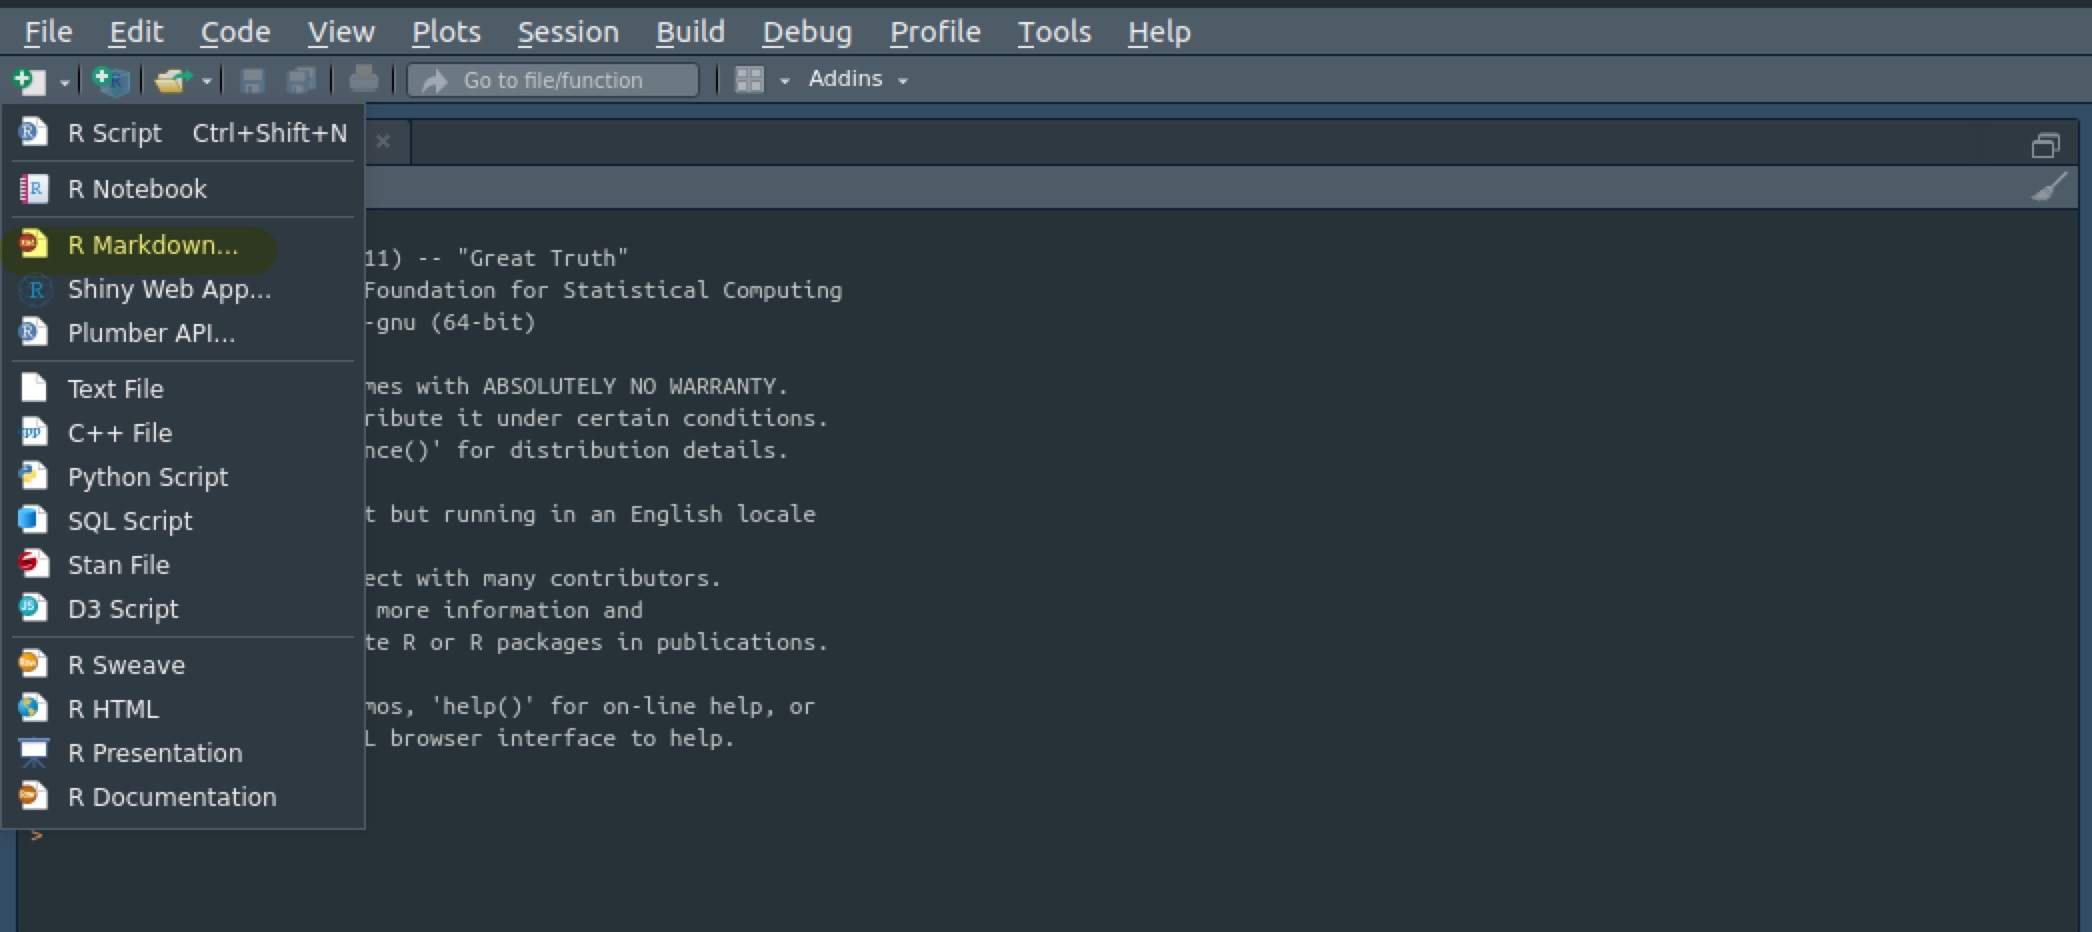
\includegraphics{figures/rmarkdown_html1.jpg}

\begin{itemize}
\tightlist
\item
  初めてR Markdownを使う場合は必要なパッケージをインストールするか聞かれるのでインストールを選択します。
\end{itemize}

続いて、どのような種類のR Markdownファイルを作成するかを選択するので、(デフォルトのままですが)\texttt{Document}の\texttt{HTML}を選択します。

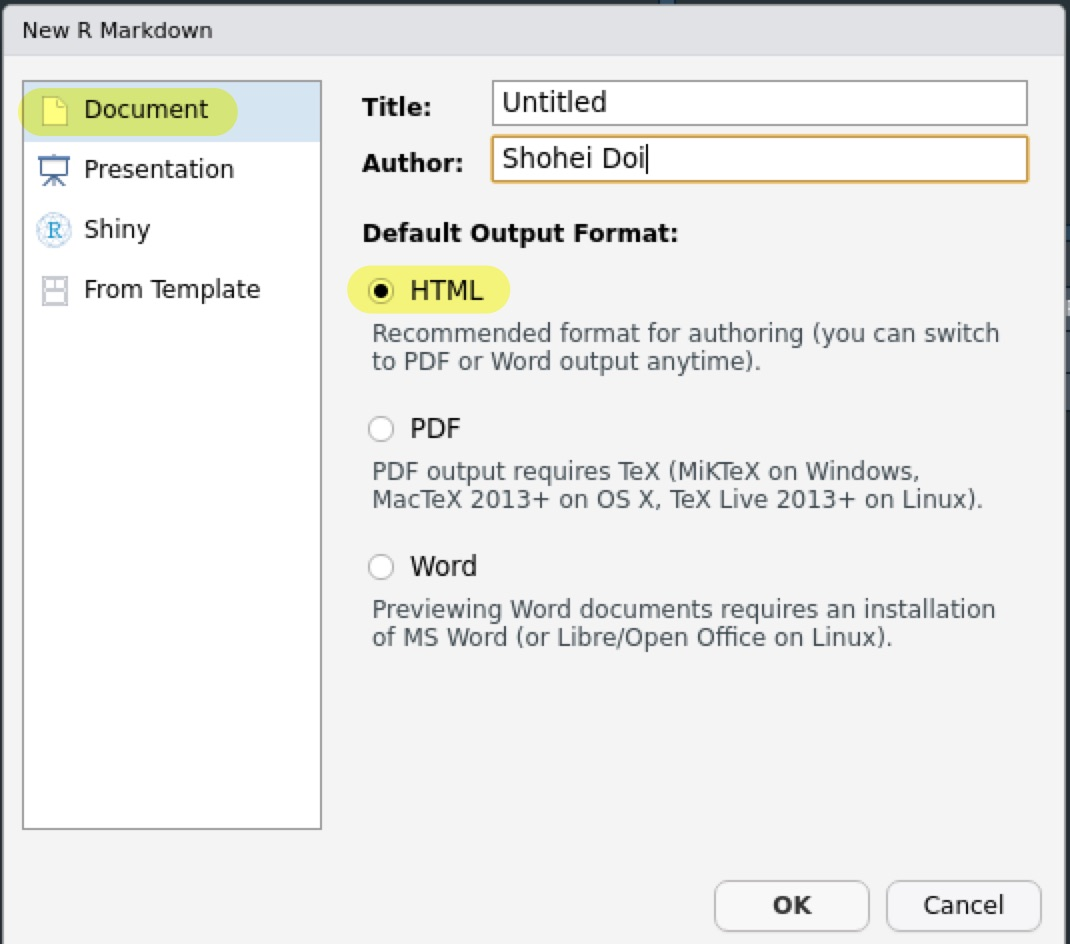
\includegraphics{figures/rmarkdown_html2.jpg}

すると、エディタに以下のようなサンプルの\texttt{Rmd}ファイルが表示されます。
適当なフォルダに保存し、エディタ上部の\texttt{Knit}をクリックするか\texttt{Shift\ +\ Ctrl\ +\ k}を押すとR Markdownファイルがタイプセットされます。

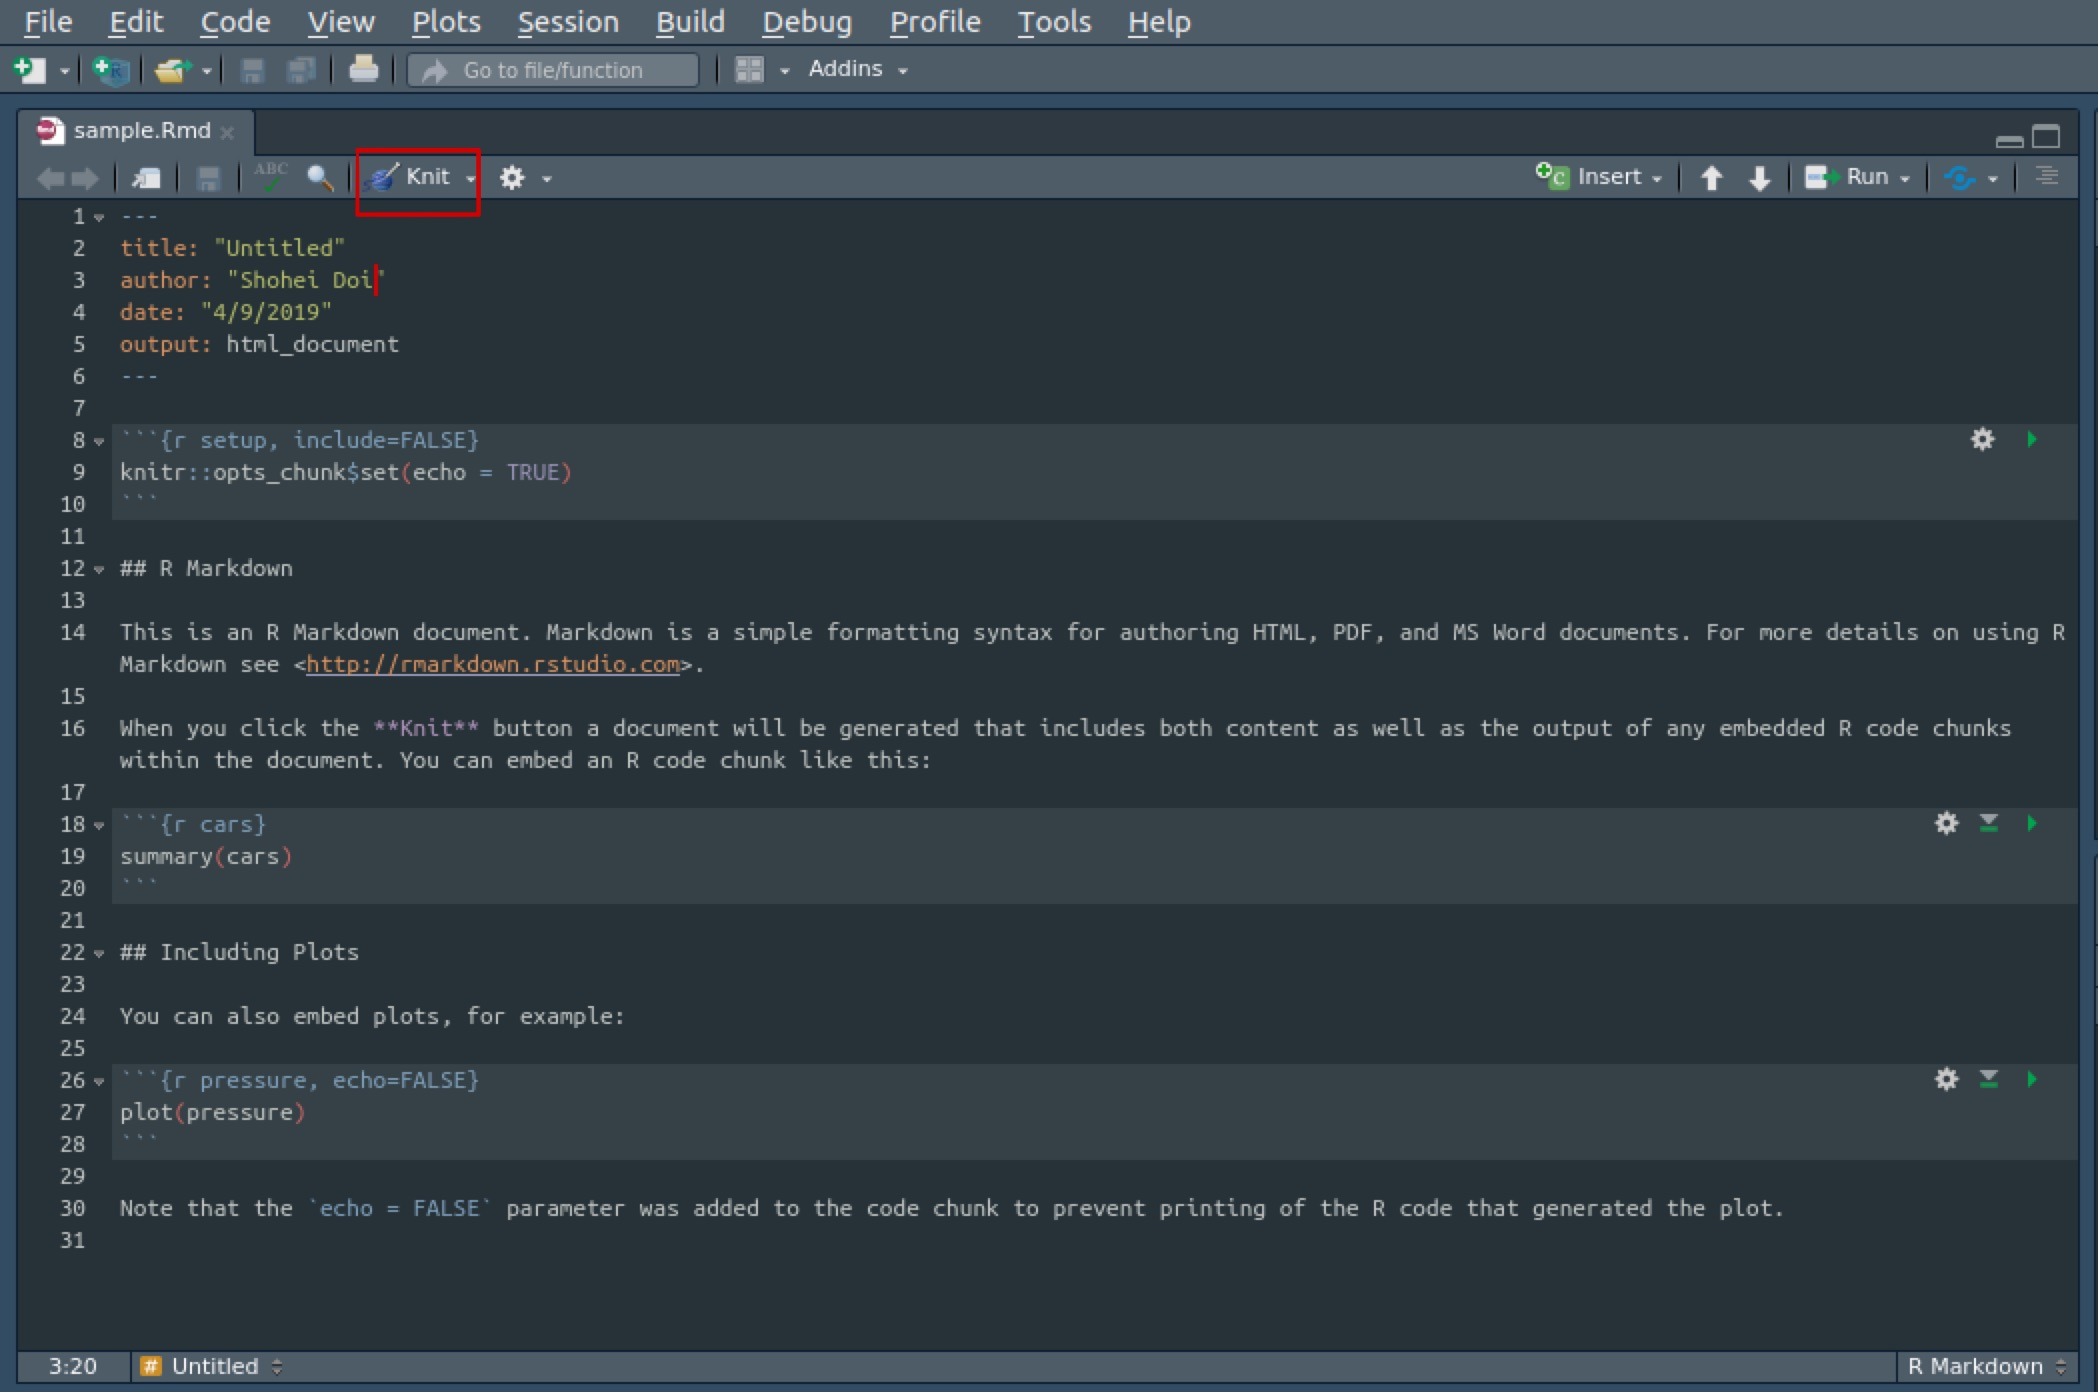
\includegraphics{figures/rmarkdown_html3.jpg}

無事、タイプセットに成功すると以下のような\texttt{.html}ファイルのプレビューが表示されます。

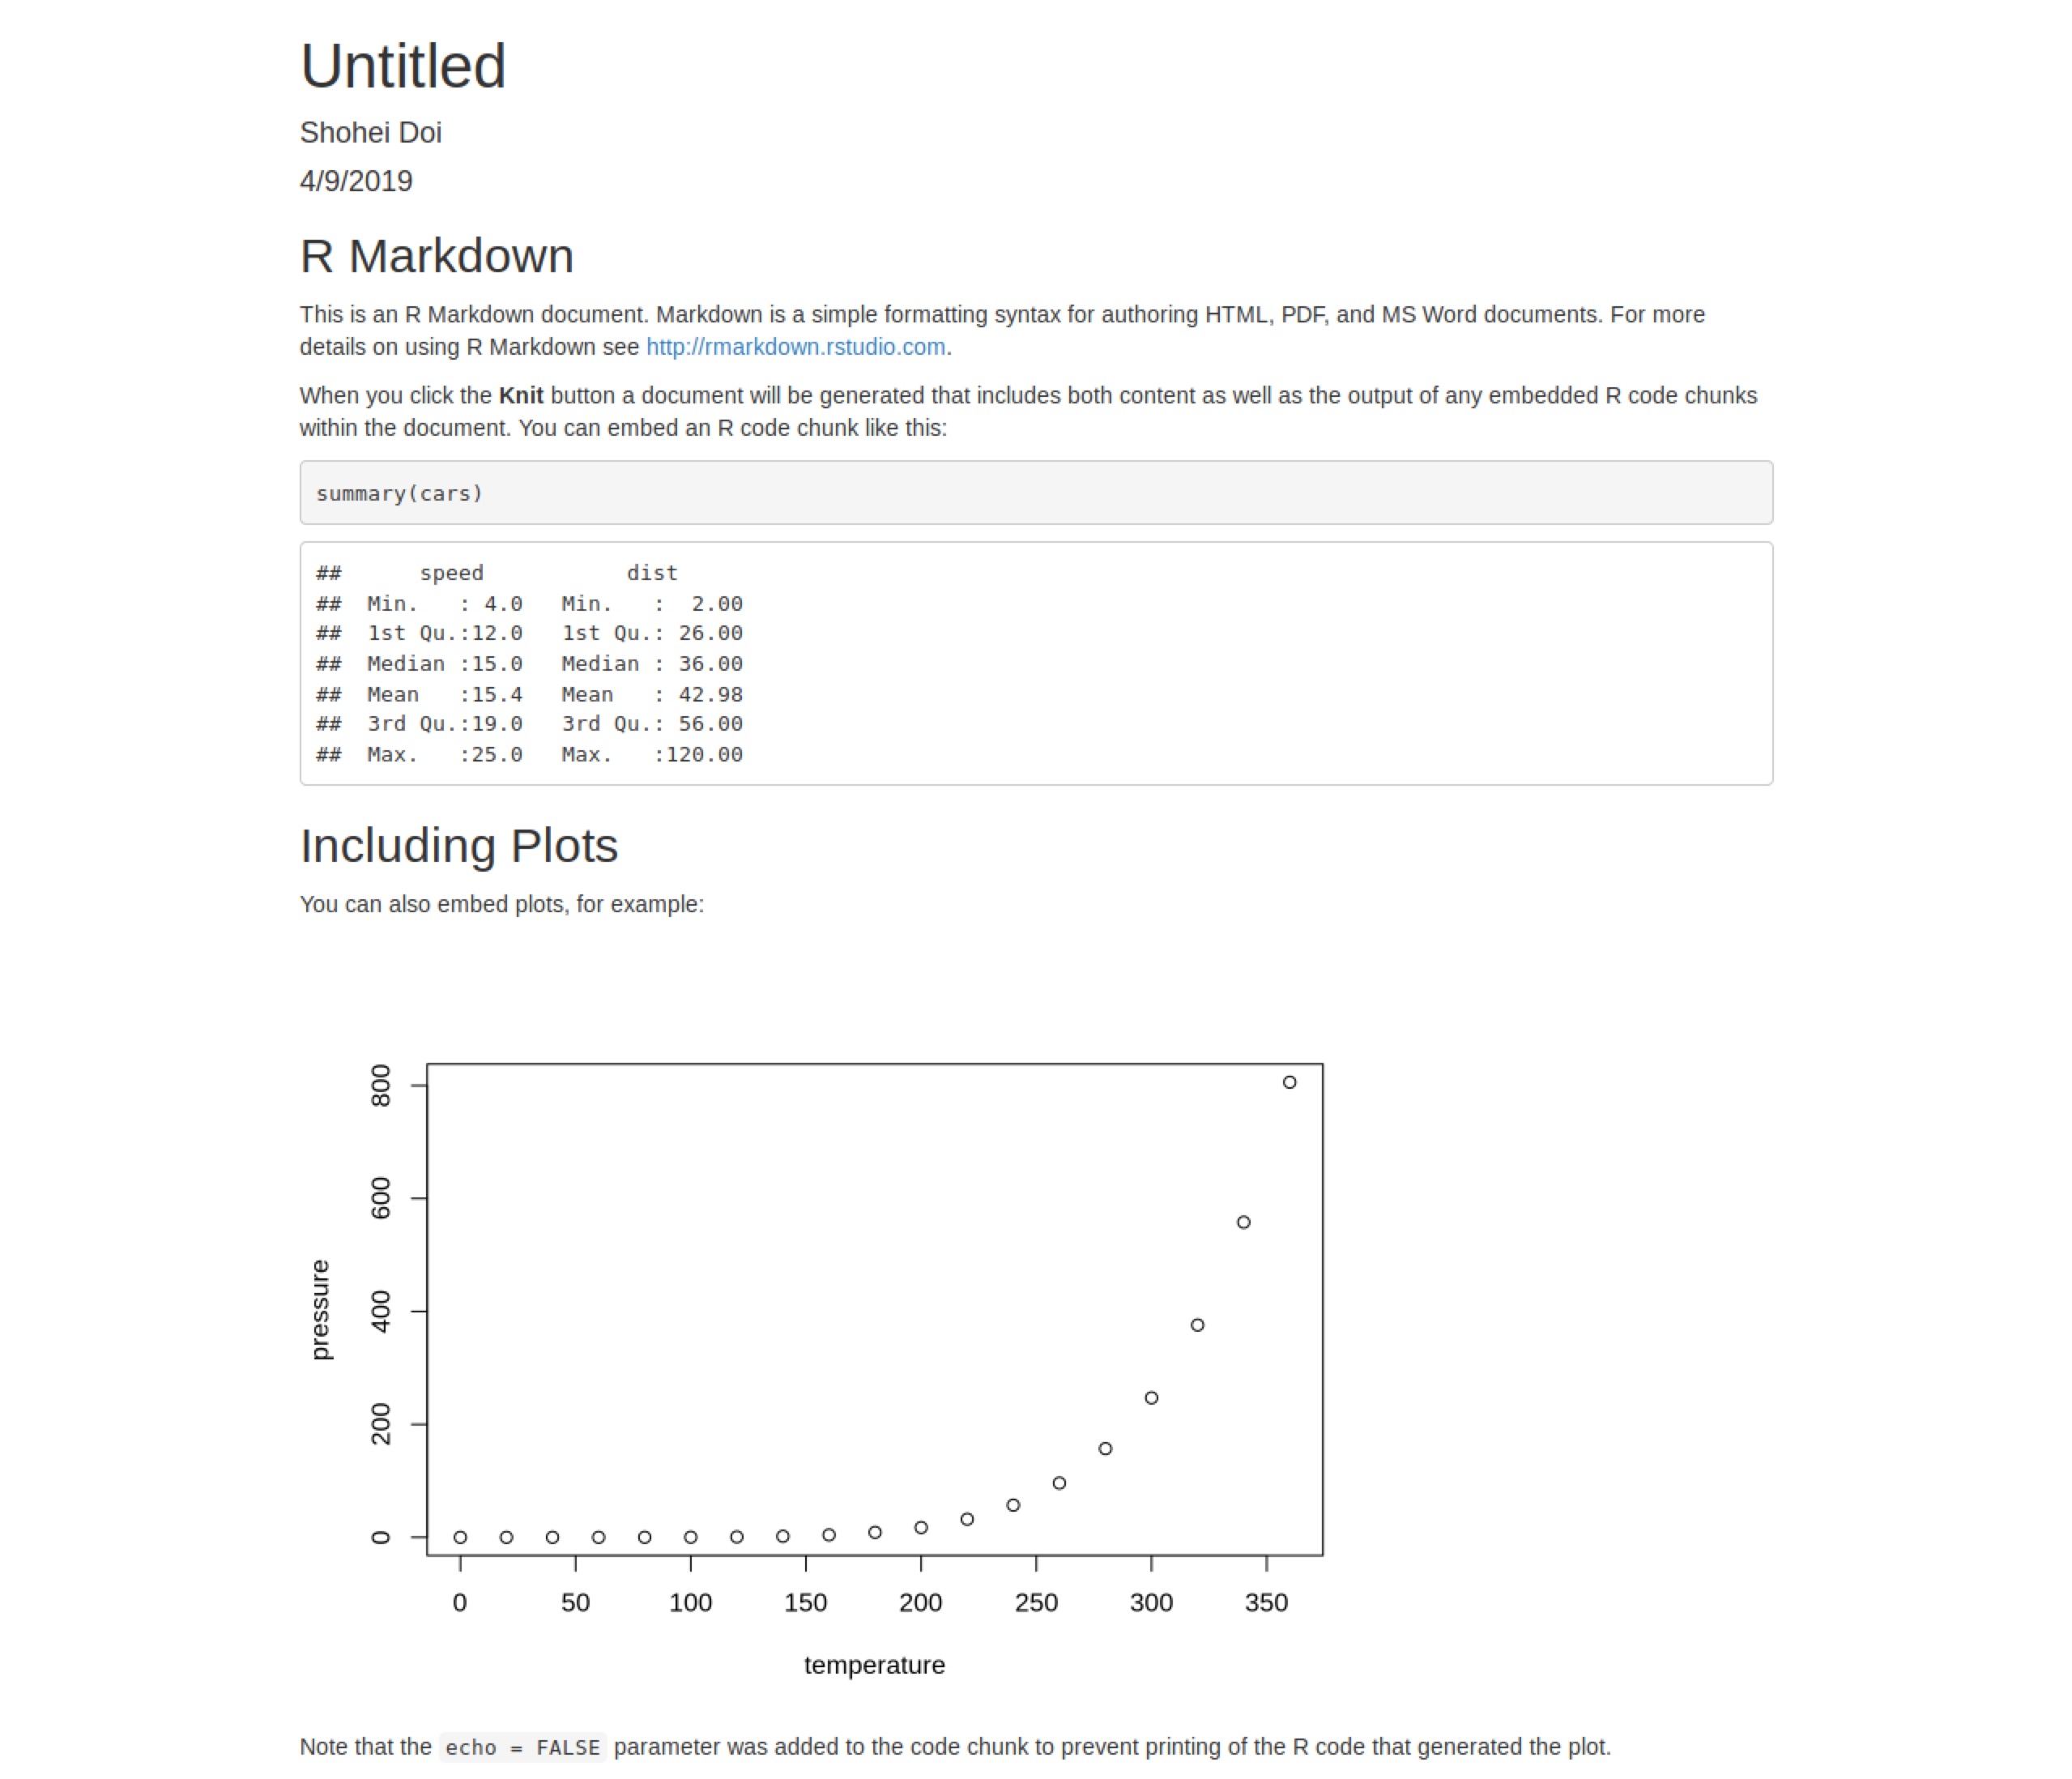
\includegraphics{figures/rmarkdown_html4.jpg}

\texttt{.Rmd}ファイルを保存したフォルダに\texttt{.html}ファイルが生成されているはずです。
\texttt{.html}ファイルとはウェブサイトを作成するためのファイルで、ウェブブラウザ(例、FirefoxやGoogle Chrome)で開くことできれいに見れます。

\hypertarget{ux53c2ux8003ux306bux306aux308bux30b5ux30a4ux30c8}{%
\subsubsection{参考になるサイト}\label{ux53c2ux8003ux306bux306aux308bux30b5ux30a4ux30c8}}

\begin{itemize}
\tightlist
\item
  \href{https://rmarkdown.rstudio.com/}{R Markdownの公式サイト}
\item
  \href{https://bookdown.org/yihui/rmarkdown/}{R Markdown: The Definitive Guide}
\item
  \href{https://www.rstudio.com/wp-content/uploads/2015/02/rmarkdown-cheatsheet.pdf}{R Markdownのチートシート (pdf)}
\item
  比治山大学の前田和寛先生の\href{https://kazutan.github.io/kazutanR/Rmd_intro.html}{R Markdown入門}
\end{itemize}

\hypertarget{Markdown}{%
\subsection{Markdown記法}\label{Markdown}}

\hypertarget{markdownux3068ux306f}{%
\subsubsection{Markdownとは*}\label{markdownux3068ux306f}}

R MarkdownとはMarkdownとRスクリプトを合体させたようなものです。
ここではMarkdownについて説明しますが、読み飛ばしても構いません。

Markdownとは計量マークアップ言語と呼ばれているように\href{https://ja.wikipedia.org/wiki/\%E3\%83\%9E\%E3\%83\%BC\%E3\%82\%AF\%E3\%82\%A2\%E3\%83\%83\%E3\%83\%97\%E8\%A8\%80\%E8\%AA\%9E}{マークアップ言語}の一種です。
マークアップ言語とは文章の中身と役割・外見を区別して記述する言語です。

逆に、世間で普及しているWordのように文章の中身と役割・外見が混在しているエディターは\href{https://ja.wikipedia.org/wiki/WYSIWYG}{WYSIWYG}と呼びます。

例えば、Wordではセクションの名前などは指定することができますが、見た目はフォントのサイズが大きくなったり、太字になったりします。
一方で、マークアップ言語の一種である\texttt{.html}ファイルでは

\begin{verbatim}
<h1>セクションタイトル</h1>
\end{verbatim}

のように明示的に\texttt{h1}というタグをつけ、\texttt{h1}タグのついている文章に対して\texttt{.css}ファイルで見た目を決定します。
同様に、LaTeXでは\texttt{\textbackslash{}section\{セクションタイトル\}}のようにタグをつけます。

基本的にはWYSIWYGなソフトのほうが直観的な操作が可能で作業が楽ではあるものの、マークアップ言語はテキストで役割や外見も決めるので再現可能性が高いと言えるでしょう。

そこで、より簡便なマークアップ言語として登場したのがMarkdown記法です。
なので、HTML記法を使うこともできます。

\hypertarget{ux30bbux30afux30b7ux30e7ux30f3}{%
\subsubsection{セクション}\label{ux30bbux30afux30b7ux30e7ux30f3}}

Markdownでは\texttt{\#}を使ってセクションのタイトルを記述します。
\texttt{\#}が多くなればなるほどより小さな見出しになります。

\begin{verbatim}
# レベル1
## レベル2
### レベル3
#### レベル4
\end{verbatim}

\hypertarget{ux30d1ux30e9ux30b0ux30e9ux30d5}{%
\subsubsection{パラグラフ}\label{ux30d1ux30e9ux30b0ux30e9ux30d5}}

空行を入れると新しいパラグラフになります。

\begin{verbatim}
同じパラグラフです。
同じパラグラフです。
\end{verbatim}

同じパラグラフです。
同じパラグラフです。

\begin{verbatim}
違うパラグラフです。

違うパラグラフです。
\end{verbatim}

違うパラグラフです。

違うパラグラフです。

\begin{itemize}
\tightlist
\item
  なので、パラグラフ内でも一文ごとに改行したほうが見やすいと思います。
\end{itemize}

\hypertarget{ux7b87ux6761ux66f8ux304d}{%
\subsubsection{箇条書き}\label{ux7b87ux6761ux66f8ux304d}}

番号なしの箇条書きの場合は\texttt{=}を、番号付きの箇条書きの場合は\texttt{1.}を入れます。

\begin{verbatim}
- 番号なし箇条書き
- 番号なし箇条書き
- 番号なし箇条書き
\end{verbatim}

\begin{itemize}
\tightlist
\item
  番号なし箇条書き
\item
  番号なし箇条書き
\item
  番号なし箇条書き
\end{itemize}

\begin{verbatim}
1. 番号付き箇条書き
1. 番号付き箇条書き
1. 番号付き箇条書き
\end{verbatim}

\begin{enumerate}
\def\labelenumi{\arabic{enumi}.}
\tightlist
\item
  番号付き箇条書き
\item
  番号付き箇条書き
\item
  番号付き箇条書き
\end{enumerate}

タブ(半角スペース4つ分)を入れると階層構造をつけることができます。

\begin{verbatim}
- レベル1
    - レベル2
- レベル1
\end{verbatim}

\begin{itemize}
\tightlist
\item
  レベル1

  \begin{itemize}
  \tightlist
  \item
    レベル2
  \end{itemize}
\item
  レベル1
\end{itemize}

\hypertarget{ux6587ux5b57ux306eux5f37ux8abf}{%
\subsubsection{文字の強調}\label{ux6587ux5b57ux306eux5f37ux8abf}}

\texttt{*}もしくは\texttt{\_}で囲むと斜体になり、\texttt{**}もしくは\texttt{\_\_}で囲むと太字になります。

\begin{verbatim}
*斜体*と**太字**
\end{verbatim}

\emph{斜体}と\textbf{太字}

\texttt{`}で囲むとコードになり、\texttt{\textasciitilde{}\textasciitilde{}}で囲むと打ち消されます。

\begin{verbatim}
`code`と~~打ち消し~~
\end{verbatim}

\texttt{code}と打ち消し

\begin{itemize}
\tightlist
\item
  日本語のLaTeXでは打ち消しに対応していないので、表示させていません。
\end{itemize}

\hypertarget{ux5f15ux7528}{%
\subsubsection{引用}\label{ux5f15ux7528}}

\texttt{\textgreater{}}から始めると引用になります。

\begin{verbatim}
> 引用文です。
\end{verbatim}

\begin{quote}
引用文です。
\end{quote}

\hypertarget{ux30eaux30f3ux30af}{%
\subsubsection{リンク}\label{ux30eaux30f3ux30af}}

リンクを貼る場合は\texttt{{[}リンク名{]}(リンク先のURL)}あるいは\texttt{\textless{}リンク先のURL\textgreater{}}とします。

\begin{verbatim}
- [RStudio](https://www.rstudio.com/)
- <https://www.rstudio.com/>
\end{verbatim}

\begin{itemize}
\tightlist
\item
  \href{https://www.rstudio.com/}{RStudio}
\item
  \url{https://www.rstudio.com/}
\end{itemize}

\hypertarget{ux753bux50cfux8868}{%
\subsubsection{画像、表}\label{ux753bux50cfux8868}}

画像を埋め込む場合は\texttt{!{[}画像名{]}(画像のパス)}とします。

\begin{verbatim}
![Rlogo](figures/Rlogo.png)
\end{verbatim}

\begin{figure}
\centering

\includegraphics{figures/Rlogo.png}
\caption{Rlogo}
\end{figure}

表を埋め込む際には次のように書きます。

\begin{verbatim}
| 項目1 | 項目2 | 項目3 |
|-------|-------|-------|
| りんご| 100   | 赤    |
| みかん| 80    | オレンジ |
\end{verbatim}

\begin{longtable}[]{@{}lll@{}}
\toprule
項目1 & 項目2 & 項目3\tabularnewline
\midrule
\endhead
りんご & 100 & 赤\tabularnewline
みかん & 80 & オレンジ\tabularnewline
\bottomrule
\end{longtable}

\hypertarget{ux6570ux5f0f}{%
\subsubsection{数式}\label{ux6570ux5f0f}}

LaTeX記法による数式を記述できます。
インラインの場合は\texttt{\$}で囲み、ディスプレイの場合は\texttt{\$\$}で囲みます。

\begin{itemize}
\tightlist
\item
  \texttt{.html}の場合、\texttt{mathjax}によって数式を表示するのでオフラインでは表示できません。
\end{itemize}

\begin{verbatim}
確率変数$X_i$は平均$\mu$、分散$\sigma^2$の正規分布に従う。
\end{verbatim}

確率変数\(X_i\)は平均\(\mu\)、分散\(\sigma^2\)の正規分布に従う。

\begin{verbatim}
$$
  X_i \sim \mathcal{N}(\mu,\sigma^2)
$$
\end{verbatim}

\[
  X_i \sim \mathcal{N}(\mu,\sigma^2)
\]

\hypertarget{Chunk}{%
\subsection{Rチャンク}\label{Chunk}}

R Markdown内でRコードを記述する際にはRチャンクと呼ばれるものの中で行います。
Rチャンクは次のような形をしています。
\texttt{Ctrl\ +\ Alt\ +\ I}でRチャンクを挿入することができます。

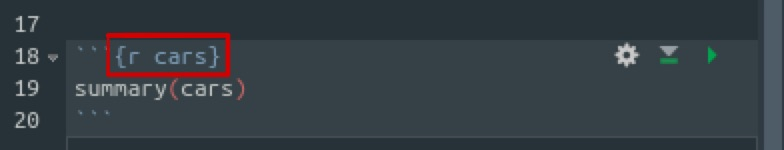
\includegraphics{figures/rmarkdown_html5_1.jpg}

まず、この部分は後述するチャンクオプションを指定する場所になります。
ここではRコードであること、チャンク名を\texttt{cars}と指定しています。

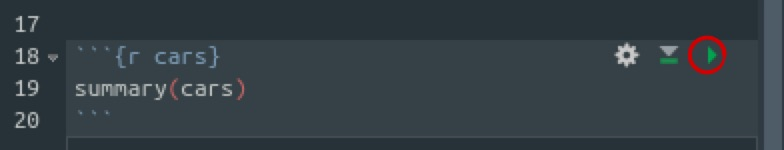
\includegraphics{figures/rmarkdown_html5_2.jpg}

R MrkdownにおいてもRスクリプトと同様に\texttt{Ctrl\ +\ Enter}でコードを実行することができます。
あるいはRチャンクの右上のボタンをクリックしても実行できます。
実行されたコードはチャンクの直下に表示されます。

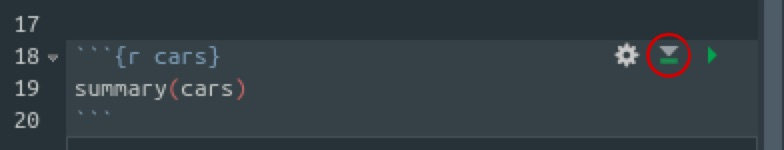
\includegraphics{figures/rmarkdown_html5_3.jpg}

右上から二番目のボタンはこのRチャンクの直前のRチャンクまでのコードを全て実行するボタンになります。

\hypertarget{ux30c1ux30e3ux30f3ux30afux30aaux30d7ux30b7ux30e7ux30f3}{%
\subsubsection{チャンクオプション}\label{ux30c1ux30e3ux30f3ux30afux30aaux30d7ux30b7ux30e7ux30f3}}

チャンクオプションを指定することでコードとそのアウトプットをどのように出力するかを制御することができます。
主なものをまとめておきます。

\begin{itemize}
\tightlist
\item
  \texttt{eval=FALSE}とするとコードは表示されるが実行されない。
\item
  \texttt{echo=FALSE}とするとコードは実行されるが表示されない。
\item
  \texttt{include=FALSE}とするとコードは実行されるがコードも実行結果も表示されない。
\item
  \texttt{warning=FALSE}や\texttt{error=FALSE}、\texttt{message=FALSE}とすると警告やエラー、メッセージが表示されない。
\end{itemize}

例えば、\texttt{\{r,\ echo=FALSE\}}のように書きます。

デフォルトを変更したい場合は冒頭で\texttt{knitr::opts\_chunk\$set(echo=TRUE)}のように設定します。

\hypertarget{YAML}{%
\subsection{yamlヘッダー}\label{YAML}}

yamlヘッダーとは\texttt{.Rmd}ファイルの冒頭で\texttt{-\/-\/-}によって囲まれた箇所で、ページ全体の設定を行います。
初期状態では

\begin{verbatim}
---
title: "Untitled"
author: "Shohei Doi"
date: "4/9/2019"
output: html_document
---
\end{verbatim}

となっていますが、\texttt{title}や\texttt{author}、\texttt{date}でタイトル、著者、日付を設定できます。

\hypertarget{output}{%
\subsubsection{output}\label{output}}

\texttt{output}によって出力形式を決定します。
これによってyamlヘッダーにおいてどのような項目を設定できるのかも決まります。

どのような出力形式が利用可能であるかは後述するとして、以下では\texttt{html\_document}における主なyamlヘッダーの設定を紹介します。

\begin{itemize}
\tightlist
\item
  前田先生の\href{https://qiita.com/kazutan/items/726e03dfcef1615ae999}{ページ}が参考になります。
\end{itemize}

\hypertarget{ux76eeux6b21}{%
\subsubsection{目次}\label{ux76eeux6b21}}

目次を出力するには次のように書きます。

\begin{verbatim}
output:
  html_document:
    toc: TRUE
\end{verbatim}

目次の設定には次のようなものがあります。

\begin{verbatim}
output:
  html_document:
    toc: TRUE
    toc_depth: 2
    toc_gloat: TRUE
    number_sections: TRUE
\end{verbatim}

\begin{itemize}
\tightlist
\item
  \texttt{toc\_depth}によってどの階層の見出しまで表示するかを決めます。
\item
  \texttt{toc\_float}を\texttt{TRUE}にすると目次がスクロールしてもついてきます。
\item
  \texttt{number\_sections}を\texttt{TRUE}にすると見出しに通し番号がつきます。
\end{itemize}

\hypertarget{ux30c6ux30fcux30de}{%
\subsubsection{テーマ}\label{ux30c6ux30fcux30de}}

テーマを決める場合は\texttt{theme}で指定します。
テーマ一覧は\href{https://bootswatch.com/3/}{こちら}になります。

\begin{verbatim}
output:
  html_document:
    theme: "paper"
\end{verbatim}

\hypertarget{htmlux3068css}{%
\subsubsection{htmlとcss}\label{htmlux3068css}}

\texttt{css}によってカスタム\texttt{.css}ファイルを指定できます。
\texttt{include}によって\texttt{.html}ファイルの挿入ができます。

デフォルトでは\texttt{.css}ファイルは画像データなどは全て\texttt{.html}ファイルに含まれてスタンドアロンな形で見ることができます。
しかし、\texttt{self\_contained}を\texttt{FALSE}とすると付属ファイルは別フォルダに作成され、\texttt{.html}ファイル自体が見やすくなります。

\hypertarget{Others}{%
\subsection{その他のテンプレート}\label{Others}}

\texttt{output}を変更することで、いくつかのテンプレートを使用することができます。
ここでは\texttt{.html}ファイルが出力されるいくつかのテンプレートを紹介しておきます。

\begin{itemize}
\tightlist
\item
  公式サイトの\href{https://rmarkdown.rstudio.com/gallery.html}{Gallery}や\href{https://rmarkdown.rstudio.com/formats.html}{Formats}をご覧ください。
\end{itemize}

\hypertarget{distill}{%
\subsubsection{Distill}\label{distill}}

\href{https://rstudio.github.io/distill/}{Distill}はウェブで公開することを念頭に置いた専門的な記事を書くためのテンプレートになっています。
インストールは以下のように行います。

\begin{Shaded}
\begin{Highlighting}[]
\NormalTok{devtools}\OperatorTok{::}\KeywordTok{install_github}\NormalTok{(}\StringTok{"rstudio/distill"}\NormalTok{)}
\end{Highlighting}
\end{Shaded}

\begin{itemize}
\tightlist
\item
  RStudioのバージョンは1.2以上であることが求められています。
\end{itemize}

インストールに成功すると\texttt{R\ Markdown...}の中の\texttt{From\ Template}に\texttt{Distill\ Article}が追加されているはずです。

\hypertarget{tufte-handout}{%
\subsubsection{Tufte Handout}\label{tufte-handout}}

\href{https://rstudio.github.io/tufte/}{Tufte Handout}というテンプレートもあります。

\begin{figure}
\centering
\includegraphics{https://bookdown.org/yihui/rmarkdown/images/tufte-overview.png}
\caption{Tufte HandoutT}
\end{figure}

\texttt{tufte}というパッケージをインストールするとテンプレートに追加されます。

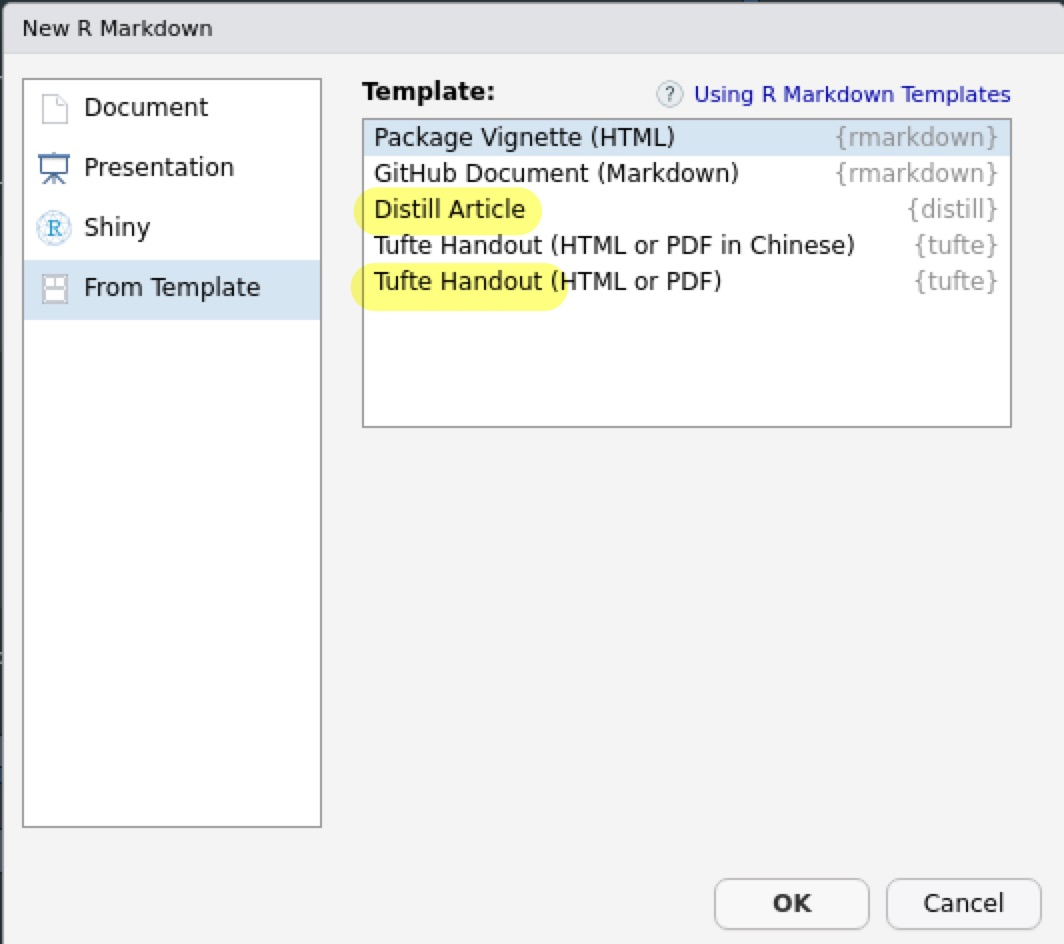
\includegraphics{figures/rmarkdown_html6.jpg}

\hypertarget{rmdformats}{%
\subsubsection{rmdformats}\label{rmdformats}}

\href{https://github.com/juba/rmdformats}{rmdformats}というテンプレートもあります。
同様に、\texttt{rmdformats}というパッケージをインストールします。

\begin{figure}
\centering
\includegraphics{https://raw.githubusercontent.com/juba/rmdformats/master/tools/screenshots/material.png}
\caption{material}
\end{figure}

\begin{figure}
\centering
\includegraphics{https://raw.githubusercontent.com/juba/rmdformats/master/tools/screenshots/readthedown.png}
\caption{readthedown}
\end{figure}

\begin{figure}
\centering
\includegraphics{https://raw.githubusercontent.com/juba/rmdformats/master/tools/screenshots/html_clean.png}
\caption{html\_clean}
\end{figure}

\begin{figure}
\centering
\includegraphics{https://raw.githubusercontent.com/juba/rmdformats/master/tools/screenshots/html_docco.png}
\caption{html\_docco}
\end{figure}

\hypertarget{ux30b9ux30e9ux30a4ux30c9}{%
\subsubsection{スライド}\label{ux30b9ux30e9ux30a4ux30c9}}

R Markdownから作成できる\texttt{.html}ファイルのスライドには\href{https://bookdown.org/yihui/rmarkdown/ioslides-presentation.html}{ioslides}と\href{https://bookdown.org/yihui/rmarkdown/slidy-presentation.html}{slidy}というものがあります。

\begin{figure}
\centering
\includegraphics{https://bookdown.org/yihui/rmarkdown/images/ioslides-1.png}
\caption{ioslides}
\end{figure}

\begin{figure}
\centering
\includegraphics{https://bookdown.org/yihui/rmarkdown/images/ioslides-2.png}
\caption{ioslides}
\end{figure}

\begin{figure}
\centering
\includegraphics{https://bookdown.org/yihui/rmarkdown/images/slidy-1.png}
\caption{slidy}
\end{figure}

\begin{figure}
\centering
\includegraphics{https://bookdown.org/yihui/rmarkdown/images/slidy-2.png}
\caption{slidy}
\end{figure}

これらはデフォルトで入っています。

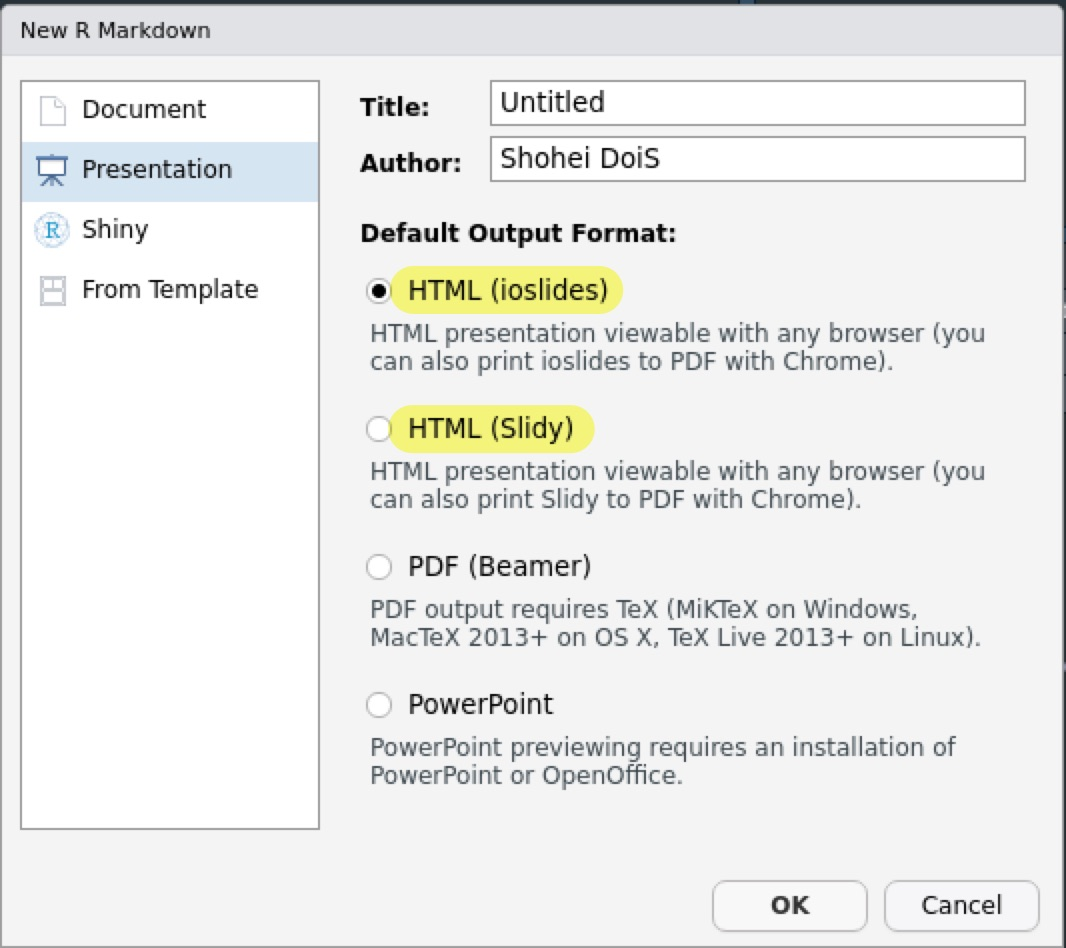
\includegraphics{figures/rmarkdown_html7.jpg}

また、\href{https://revealjs.com/}{reveal.js}という\texttt{.html}スライドを作ることもできます。
\texttt{revealjs}というパッケージをインストールするとテンプレートが追加されます。

\begin{itemize}
\tightlist
\item
  \texttt{Presentation}の方ではない点に注意。
\end{itemize}

\begin{figure}
\centering
\includegraphics{https://bookdown.org/yihui/rmarkdown/images/revealjs-1.png}
\caption{reveal.js}
\end{figure}

\begin{figure}
\centering
\includegraphics{https://bookdown.org/yihui/rmarkdown/images/revealjs-2.png}
\caption{reveal.js}
\end{figure}

同様にして\href{https://github.com/yihui/xaringan}{xaringan}というNARUTOという忍者マンガにインスパイアされたテンプレートを使用することもできます。

\begin{figure}
\centering
\includegraphics{https://bookdown.org/yihui/rmarkdown/images/xaringan-1.png}
\caption{xaringan}
\end{figure}

\begin{figure}
\centering
\includegraphics{https://bookdown.org/yihui/rmarkdown/images/xaringan-2.png}
\caption{xaringan}
\end{figure}

\hypertarget{Dashboard}{%
\subsubsection{ダッシュボード}\label{Dashboard}}

\texttt{flexdashboard}というパッケージを使うと\href{https://rmarkdown.rstudio.com/flexdashboard/}{ダッシュボード}を作ることができます。
パッケージをインストールすると\texttt{Flex\ Dashboard}というテンプレートが追加されます。

\begin{figure}
\centering
\includegraphics{https://rmarkdown.rstudio.com/flexdashboard/images/htmlwidgets-d3heatmap.png}
\caption{flexdashboard}
\end{figure}

\hypertarget{microsoft-office}{%
\subsubsection{Microsoft Office}\label{microsoft-office}}

R MarkdownからMicrosoft OfficeのWordやPowerPointの形式のファイルを作成することも可能です。

\hypertarget{encoding-r}{%
\section{Rにおける文字コード*}\label{encoding-r}}

Rに限らず文字化けはPCにおいてしばしば起こる問題です。
平たく言ってしまうと、PCでは文字にコードが付与されており、機械がコードを読み取って文字を表示します。
そのコードと文字の対応関係をエンコーディングと呼び、異なるエンコーディングでデータを読み込むと文字化けが起こります。

\hypertarget{ux306aux305cux6587ux5b57ux5316ux3051ux304cux8d77ux3053ux308bux306eux304b}{%
\subsection{なぜ文字化けが起こるのか}\label{ux306aux305cux6587ux5b57ux5316ux3051ux304cux8d77ux3053ux308bux306eux304b}}

\hypertarget{ux30a8ux30f3ux30b3ux30fcux30c7ux30a3ux30f3ux30b0}{%
\subsubsection{エンコーディング}\label{ux30a8ux30f3ux30b3ux30fcux30c7ux30a3ux30f3ux30b0}}

実用上、日本語で文字化けが起こる問題の大半は

\begin{itemize}
\tightlist
\item
  Windowsでは\texttt{Shift-JIS}あるいは\texttt{CP932}で、
\item
  LinuxやMacなどのUNIX系では\texttt{UTF-8}で
\end{itemize}

エンコーディングしていることに起因しています。

\texttt{UTF-8}の\texttt{U}は\texttt{unicode}であることからも分かるように、世界で共通の規格として作られているエンコーディング方式になります。
なので、RおよびRStudioでは日本語独自の\texttt{Shift-JIS}ではなく\texttt{UTF-8}を使うようにしたほうがよいでしょう。

\hypertarget{rux3068rstudioux306bux304aux3051ux308bux554fux984c}{%
\subsubsection{RとRStudioにおける問題}\label{rux3068rstudioux306bux304aux3051ux308bux554fux984c}}

RとRStudioで文字化けが起こる問題は大きく2つに分けられます。

\begin{enumerate}
\def\labelenumi{\arabic{enumi}.}
\tightlist
\item
  RStudioで日本語を含むRスクリプトを開いたとき
\item
  Rで日本語を含むデータを読み込んだとき
\end{enumerate}

以下では、それぞれの問題の対処法を紹介します。

\hypertarget{rux30b9ux30afux30eaux30d7ux30c8ux306eux6587ux5b57ux5316ux3051}{%
\subsection{Rスクリプトの文字化け}\label{rux30b9ux30afux30eaux30d7ux30c8ux306eux6587ux5b57ux5316ux3051}}

Rスクリプトが文字化けしている場合はRStudiで対処します。
例として\href{script/script_utf8.R}{\texttt{UTF-8}でエンコードしたRスクリプト}と\href{script/script_sjis.R}{\texttt{Shift-JIS}でエンコードしたRスクリプト}をRStudioで開いてみてください。
(設定を変更していなければ)Windowsの場合は前者が、Linux/Macの人は後者が文字化けしているはずです。

\hypertarget{ux30d5ux30a1ux30a4ux30ebux3092ux958bux304f}{%
\subsubsection{ファイルを開く}\label{ux30d5ux30a1ux30a4ux30ebux3092ux958bux304f}}

まず、デフォルトを\texttt{UTF-8}に変更しましょう。
メニューの中の\texttt{File}に\texttt{Reopen\ with\ Encoding...}というのがあるので、\texttt{UTF-8}を選択します。
さらに\texttt{Set\ as\ default\ encoding\ for\ source\ files}にチェックを入れることで今後は\texttt{UTF-8}で表示されます。

\texttt{UTF-8}でエンコードされた方は正常に表示され、\texttt{Shift-JIS}でエンコードされた方は文字化けしていることを確認してください。
今後、RStudioで文字化けが起こる場合はデフォルトが\texttt{UTF-8}になっているので、Rスクリプトが他のエンコードのために起こっていることになります。

そのような場合には\texttt{Reopen\ with\ Encoding...}で適当なエンコーディングを選択します。
例えば、\texttt{Shift-JIS}を選択すると正しく表示されるはずです。

\hypertarget{ux30d5ux30a1ux30a4ux30ebux3092ux4fddux5b58ux3059ux308b}{%
\subsubsection{ファイルを保存する}\label{ux30d5ux30a1ux30a4ux30ebux3092ux4fddux5b58ux3059ux308b}}

自分で作成したRスクリプトを保存する際にはメニューの\texttt{File}の中の\texttt{Save\ with\ Encoding...}で\texttt{UTF-8}を選択してください。
ここでも\texttt{UTF-8}がデフォルトになるようにチェックを入れておきましょう。

\hypertarget{ux30c7ux30fcux30bfux306eux6587ux5b57ux5316ux3051}{%
\subsection{データの文字化け}\label{ux30c7ux30fcux30bfux306eux6587ux5b57ux5316ux3051}}

データが文字化けしているときはRで対処します。
\href{data/data_utf8.csv}{\texttt{UTF-8}でエンコーディングしたデータ}と\href{data/data_sjis.csv}{\texttt{Shift-JIS}でエンコーディングしたデータ}をそれぞれ読み込んでみてください。
やはりWindowsでは前者が、Linux/Macでは後者が文字化けをしているはずです。

\begin{Shaded}
\begin{Highlighting}[]
\KeywordTok{read.csv}\NormalTok{(}\StringTok{"data/data_utf8.csv"}\NormalTok{)}
\end{Highlighting}
\end{Shaded}

\begin{verbatim}
##   member
## 1   イヌ
## 2   サル
## 3   キジ
\end{verbatim}

\begin{Shaded}
\begin{Highlighting}[]
\KeywordTok{read.csv}\NormalTok{(}\StringTok{"data/data_sjis.csv"}\NormalTok{)}
\end{Highlighting}
\end{Shaded}

\begin{verbatim}
## Error in type.convert.default(data[[i]], as.is = as.is[i], dec = dec, : invalid multibyte string at '<83>C<83>k'
\end{verbatim}

\begin{itemize}
\tightlist
\item
  僕はLinuxを使っているので後者が文字化けを起こしてエラーが出ています。
\end{itemize}

\hypertarget{ux6a19ux6e96ux95a2ux6570ux306eux5834ux5408}{%
\subsubsection{標準関数の場合}\label{ux6a19ux6e96ux95a2ux6570ux306eux5834ux5408}}

標準関数の場合、\texttt{fileEncoding}というオプションでエンコーディングを指定します。

\begin{Shaded}
\begin{Highlighting}[]
\KeywordTok{read.csv}\NormalTok{(}\StringTok{"data/data_utf8.csv"}\NormalTok{, }\DataTypeTok{fileEncoding =} \StringTok{"utf8"}\NormalTok{)}
\end{Highlighting}
\end{Shaded}

\begin{verbatim}
##   member
## 1   イヌ
## 2   サル
## 3   キジ
\end{verbatim}

\begin{Shaded}
\begin{Highlighting}[]
\KeywordTok{read.csv}\NormalTok{(}\StringTok{"data/data_sjis.csv"}\NormalTok{, }\DataTypeTok{fileEncoding =} \StringTok{"shift-jis"}\NormalTok{)}
\end{Highlighting}
\end{Shaded}

\begin{verbatim}
##   member
## 1   イヌ
## 2   サル
## 3   キジ
\end{verbatim}

\hypertarget{tidyverseux306eux5834ux5408}{%
\subsubsection{tidyverseの場合}\label{tidyverseux306eux5834ux5408}}

\texttt{tidyverse}の\texttt{readr}の場合は\texttt{locale}で指定します。

\begin{itemize}
\tightlist
\item
  \texttt{readr}は\texttt{tidyverse}に含まれているので、\texttt{tidyverse}を読み込んだ場合は、別途読み込む必要はありません。
\end{itemize}

\begin{Shaded}
\begin{Highlighting}[]
\KeywordTok{library}\NormalTok{(tidyverse)}
\KeywordTok{read_csv}\NormalTok{(}\StringTok{"data/data_utf8.csv"}\NormalTok{, }\DataTypeTok{locale =} \KeywordTok{locale}\NormalTok{(}\DataTypeTok{encoding =} \StringTok{"utf8"}\NormalTok{))}
\end{Highlighting}
\end{Shaded}

\begin{verbatim}
## Parsed with column specification:
## cols(
##   member = col_character()
## )
\end{verbatim}

\begin{verbatim}
## # A tibble: 3 x 1
##   member
##   <chr> 
## 1 イヌ  
## 2 サル  
## 3 キジ
\end{verbatim}

\begin{Shaded}
\begin{Highlighting}[]
\KeywordTok{read_csv}\NormalTok{(}\StringTok{"data/data_sjis.csv"}\NormalTok{, }\DataTypeTok{locale =} \KeywordTok{locale}\NormalTok{(}\DataTypeTok{encoding =} \StringTok{"shift-jis"}\NormalTok{))}
\end{Highlighting}
\end{Shaded}

\begin{verbatim}
## Parsed with column specification:
## cols(
##   member = col_character()
## )
\end{verbatim}

\begin{verbatim}
## # A tibble: 3 x 1
##   member
##   <chr> 
## 1 イヌ  
## 2 サル  
## 3 キジ
\end{verbatim}

\hypertarget{ux30a8ux30f3ux30b3ux30fcux30c7ux30a3ux30f3ux30b0ux3092ux78baux8a8dux3059ux308bux65b9ux6cd5}{%
\subsubsection{エンコーディングを確認する方法}\label{ux30a8ux30f3ux30b3ux30fcux30c7ux30a3ux30f3ux30b0ux3092ux78baux8a8dux3059ux308bux65b9ux6cd5}}

\texttt{readr}の\texttt{guess\_encoding()}という関数を使うと、どのようなエンコーディングがされているかを推測します。

\begin{Shaded}
\begin{Highlighting}[]
\KeywordTok{guess_encoding}\NormalTok{(}\StringTok{"data/data_utf8.csv"}\NormalTok{)}
\end{Highlighting}
\end{Shaded}

\begin{verbatim}
## # A tibble: 1 x 2
##   encoding confidence
##   <chr>         <dbl>
## 1 UTF-8             1
\end{verbatim}

\begin{Shaded}
\begin{Highlighting}[]
\KeywordTok{guess_encoding}\NormalTok{(}\StringTok{"data/data_sjis.csv"}\NormalTok{)}
\end{Highlighting}
\end{Shaded}

\begin{verbatim}
## # A tibble: 1 x 2
##   encoding     confidence
##   <chr>             <dbl>
## 1 windows-1252       0.35
\end{verbatim}

\begin{itemize}
\tightlist
\item
  \texttt{windows-1215}というのはCP1215とも呼ばれるエンコーディングで、Shift-JISの親戚のようなものです(きっと)。
\end{itemize}

\hypertarget{ux3082ux3068ux306eux30c7ux30fcux30bfux3092ux898bux305fux3044ux5834ux5408}{%
\subsubsection{もとのデータを見たい場合}\label{ux3082ux3068ux306eux30c7ux30fcux30bfux3092ux898bux305fux3044ux5834ux5408}}

しばしばRではなく直接データを見たいときがあります。
そのような場合は、\href{https://ja.libreoffice.org/}{LibreOffice}のCalcというソフトで開くとエンコーディングを指定することができます。

\hypertarget{ux30c7ux30fcux30bfux3092ux4fddux5b58ux3059ux308bux5834ux5408}{%
\subsubsection{データを保存する場合}\label{ux30c7ux30fcux30bfux3092ux4fddux5b58ux3059ux308bux5834ux5408}}

データを書き出す場合、\texttt{UTF-8}で行うのが望ましいですが、そうするとWindowsからExcelなどで開いた場合に文字化けしてしまいます。
それを回避するために、\texttt{readr}の\texttt{write\_excel\_csv()}を使うとエクセルで開いても文字化けしません。

\hypertarget{Others}{%
\subsection{その他の問題}\label{Others}}

\hypertarget{ux30a2ux30abux30a6ux30f3ux30c8ux540dux304cux65e5ux672cux8a9eux306eux5834ux5408}{%
\subsubsection{アカウント名が日本語の場合}\label{ux30a2ux30abux30a6ux30f3ux30c8ux540dux304cux65e5ux672cux8a9eux306eux5834ux5408}}

Windowsでアカウント名が日本語の場合、パスを通すときにエラーが出てくる場合があります。
そのような場合は、

\begin{enumerate}
\def\labelenumi{\arabic{enumi}.}
\tightlist
\item
  新しいアカウントを作成する。
\item
  新しいアカウントを作成し、現在のアカウントの内容を全てコピーして、現在のアカウントを削除する。
\item
  OSをクリーンインストールする。
\item
  Linux(Ubuntuなど)を使う。

  \begin{enumerate}
  \def\labelenumii{\arabic{enumii}.}
  \tightlist
  \item
    仮想マシン(VMwareやVirtualBox)を使う。
  \item
    デュアルブートをする。
  \end{enumerate}
\end{enumerate}

といった選択肢が考えられます(下に行くほど難易度が高い)。

\hypertarget{ux753bux50cfux3067ux65e5ux672cux8a9eux304cux6587ux5b57ux5316ux3051ux3059ux308bux5834ux5408}{%
\subsubsection{画像で日本語が文字化けする場合}\label{ux753bux50cfux3067ux65e5ux672cux8a9eux304cux6587ux5b57ux5316ux3051ux3059ux308bux5834ux5408}}

Macで画像を出力する際に日本語が文字化けすることがあります。
\texttt{plot()}の場合は、

\begin{Shaded}
\begin{Highlighting}[]
\KeywordTok{par}\NormalTok{(}\DataTypeTok{family =} \StringTok{"HiraKakuProN-W3"}\NormalTok{)}
\end{Highlighting}
\end{Shaded}

\texttt{ggplot2}の場合は、

\begin{Shaded}
\begin{Highlighting}[]
\KeywordTok{theme}\NormalTok{(}\DataTypeTok{base_family =} \StringTok{"HiraKakuProN-W3"}\NormalTok{)}
\end{Highlighting}
\end{Shaded}

とするらしいです(Macは使ったことがないので分かりません)。

\begin{itemize}
\tightlist
\item
  \texttt{quanteda}でプロットする際、うまくフォントが指定できない場合があるので、\href{https://github.com/quanteda/quanteda/issues/1317}{こちら}を参考に、\texttt{extrafont::fonts()}でフォント一覧を確認して、適当なものを指定して下さい。
\end{itemize}

\hypertarget{environment}{%
\section*{動作環境}\label{environment}}
\addcontentsline{toc}{section}{動作環境}

\begin{Shaded}
\begin{Highlighting}[]
\KeywordTok{sessionInfo}\NormalTok{()}
\end{Highlighting}
\end{Shaded}

\begin{verbatim}
## R version 3.6.3 (2020-02-29)
## Platform: x86_64-pc-linux-gnu (64-bit)
## Running under: Ubuntu 18.04.4 LTS
## 
## Matrix products: default
## BLAS:   /usr/lib/x86_64-linux-gnu/blas/libblas.so.3.7.1
## LAPACK: /usr/lib/x86_64-linux-gnu/lapack/liblapack.so.3.7.1
## 
## locale:
##  [1] LC_CTYPE=en_US.UTF-8       LC_NUMERIC=C              
##  [3] LC_TIME=en_US.UTF-8        LC_COLLATE=en_US.UTF-8    
##  [5] LC_MONETARY=en_US.UTF-8    LC_MESSAGES=en_US.UTF-8   
##  [7] LC_PAPER=en_US.UTF-8       LC_NAME=C                 
##  [9] LC_ADDRESS=C               LC_TELEPHONE=C            
## [11] LC_MEASUREMENT=en_US.UTF-8 LC_IDENTIFICATION=C       
## 
## attached base packages:
## [1] stats     graphics  grDevices utils     datasets  methods   base     
## 
## other attached packages:
## [1] forcats_0.5.0   stringr_1.4.0   dplyr_0.8.5     purrr_0.3.4    
## [5] readr_1.3.1     tidyr_1.0.2     tibble_3.0.0    ggplot2_3.3.0  
## [9] tidyverse_1.3.0
## 
## loaded via a namespace (and not attached):
##  [1] tidyselect_1.0.0 xfun_0.13        haven_2.2.0      lattice_0.20-41 
##  [5] colorspace_1.4-1 vctrs_0.2.4      generics_0.0.2   htmltools_0.4.0 
##  [9] yaml_2.2.1       utf8_1.1.4       rlang_0.4.5      pillar_1.4.3    
## [13] withr_2.1.2      glue_1.4.0       DBI_1.1.0        dbplyr_1.4.3    
## [17] modelr_0.1.6     readxl_1.3.1     lifecycle_0.2.0  munsell_0.5.0   
## [21] gtable_0.3.0     cellranger_1.1.0 rvest_0.3.5      evaluate_0.14   
## [25] knitr_1.28       fansi_0.4.1      highr_0.8        broom_0.5.5     
## [29] Rcpp_1.0.4.6     backports_1.1.6  scales_1.1.0     jsonlite_1.6.1  
## [33] fs_1.4.1         hms_0.5.3        digest_0.6.25    stringi_1.4.6   
## [37] bookdown_0.18    grid_3.6.3       cli_2.0.2        tools_3.6.3     
## [41] magrittr_1.5     crayon_1.3.4     pkgconfig_2.0.3  ellipsis_0.3.0  
## [45] xml2_1.3.1       reprex_0.3.0     lubridate_1.7.8  assertthat_0.2.1
## [49] rmarkdown_2.1    httr_1.4.1       rstudioapi_0.11  R6_2.4.1        
## [53] nlme_3.1-144     compiler_3.6.3
\end{verbatim}

\bibliography{book.bib}

\end{document}
